\documentclass[shuuron]{kuee}
\usepackage[dvipdfmx]{graphicx}
\usepackage{lineno,hyperref}
\usepackage{kueecite}
\usepackage{url}

\title{心理カウンセリングの\\品質向上を支援する\\視覚的分析に関する研究}
\author{上辻智也}
\professor{小山田 耕二 教授}
\course{京都大学大学院工学研究科}
\department{電気工学専攻}
\date{平成30年2月1日}




%%abstract.texの中身



%%% 本文
\begin{document}
\maketitle
\tableofcontents

% \begin{eabstract}
%   \begin{flushleft}
\Large
Visual analysis supporting quality improvement of psychological counseling
\end{flushleft}
\begin{flushright}
Tomoya Uetsuji, \\
Graduate School of Engineering, \\
Deparment of Electrical Engineering,\\
Kyoto University
\end{flushright}
\hspace{20zw}
In psychological counseling, treatment is offered to a psychosomatic patient or client mainly due to the physical symptoms caused by stress. However, beginner counselors often have difficulty turning their attention to the cognitive characteristics of the internal problems faced by clients.

 Therefore, expert counselors provide an opportunity for education and training by offering advice to beginner counselors on the content of their counseling conversations. However, due to privacy and client confidentiality issues, experts can rarely obtain voice data from beginner counselors' psychological counseling sessions. Therefore, it is usual for expert counselors to only read direct phonetic transcriptions of conversation of counseling sessions in supervision to support the education of beginner counselors.

However, transcript documents that comprise the text data of conversations in psychological counseling are large in scale and complex. It is very difficult for the supervisor to extract the conversational characteristics from the situation that exists between a beginner counselor and a client by referring to such data. To improve the accessibility of counseling conversations, we propose that visualization of data is more effective. Accordingly, we have developed an appropriate method to visualize the client's answers to each of the beginner counselor's questions. We considered how the limitation in the current supervision for beginner counselors about how to conduct successful counseling conversations can be reduced. In addition, we considered how the supervision for beginner counsellors can be improved using counseling transcripts.

 In addition, if you are interested in changing your own behavior rather than changing the behavior of the opponent, cognitive correction is progressing Therefore, we propose that classifying the client's behavior according to the information provided by the counseling conversation data, and then visualizing the result, reveals the degree of modification of the client's perception and cognition in psychological counseling. we visualized the conversation data using a method that combines a curcular human relationship chart with the behavior enacted by the people discussed in the psychological counseling conversation. We considered that counselors can check the condition of cognitive correction by our proposed time-series visualization of circular-link human relationship chart with behavior arrows.

% \end{eabstract}

%%%序論
\chapter{序論}

心療において,カウンセラーは心身症やストレスからくる身体症状をもつ患者やクライエント(以降,「患者やクライエント」を「クライエント」と統一する)に対して心理カウンセリングを行う.
心理カウンセリングでは,クライエントが抱いている,いわゆる「対人関係上の問題」にカウンセラーが自身の関心を向けて傾聴するということが基本とされる\cite{zokad}.一方,心理カウンセリングを進めていく中で,クライエントのが相手の言動を変えることより,自分の言動を変えていくことに関心が向くことで,クライエントの認知の修正が進行しているといわれている\cite{Darshana}.本研究ではこれらの要素を心理カウンセリングの品質向上のために重要な要素として取り扱う.

%そこで,心理カウンセリングにおいて, カウンセラーは,主にストレスの原因による物理的な症状に悩むクライエントに対して心理カウンセリングを提供している.心理カウンセリングの会話は音声ないし動画として記録され,後述するカウンセラー指導・事例検討の目的で役立てられているが,クライエントのプライバシーの関係上,実際の事例検討やカウンセラー教育の場では,それを書き起こした逐語録を用いることが多い.

%%品質の定義

% 武藤ら\cite{武藤清栄2007人間関係やコミュニケーション障害による生産性の低下}は医療に携わる人間のコミュニケーション能力の低下が心理カウンセリングを含むサービス業としての医療の品質の低下につながるとしている.
心理カウンセリングの品質向上のために,会話記録を基に熟練カウンセラーが初心者のカウンセラーに対して指導やアドバイスを行う機会として,スーパービジョンと呼ばれる事例検討会が行われている.スーパービジョンでは,熟練カウンセラー(スーパーヴァイザー)が初心者のカウンセラー(スーパーヴァイジー)に対して,クライエントと初心者のカウンセラーとの心理カウンセリングの会話記録を基に指導を行うのが一般的な流れである.%植田ら\cite{植田一博2006会話の分析とモデル化}は心理カウンセリング中の非言語行動から品質の導出を試みたが,テキストからはそのような非言語行動が読めない.

% 今回取り扱うヨーガ療法において鎌田ら\cite{Darshana}によれば,心理カウンセリングの目的はクライエントの認知を修正することであるが,初心者のカウンセラーはクライエントが抱いている問題に自分の関心を傾聴することが困難であり,したがってクライエントの認知を修正する段階までいくのが困難である.
% そこで本研究で説明する心理カウンセリングの品質とは,下記の2つの項目によって構成されるものとする.
% \begin{itemize}
%   \item カウンセラーの関心がどの程度クライエントが抱いている問題に傾聴されているか
%   \item クライエントの認知の修正がどの程度進行しているか
% \end{itemize}

% 熟練カウンセラーから初心者のカウンセラーへの指導をスーパービジョンと呼び,指導する側である熟練カウンセラーはスーパーヴァイザー,指導される側である初心者のカウンセラーはスーパーヴァイジ―と呼ばれるが,クライエントと初心者のカウンセラーとの心理カウンセリングの会話記録を基に熟練カウンセラーが初心者のカウンセラーに対して指導を行う,というのがスーパービジョンの流れである.
心理カウンセリングの会話記録はカウンセラー教育・事例検討を目的として,心理カウンセリング中の音声や動画が撮影される.しかし,プライバシーの関係上,それらをテキストに書き起こした逐語録を作成して,スーパービジョンで用いられることが多い.しかし,熟練カウンセラーが逐語録の文字を読むだけでは心理カウンセリングの会話の流れを把握することが難しく,クライエントが抱える問題に対して初心者のカウンセラーの関心がどの程度傾聴されているかなどの内容が十分に行えていない問題が生じている.

%具体的な理由
%・例えば:一長一短では治らない.こんなに閉じられた質問をしていたのかという実感が沸かない.

さらに,同じクライエントとカウンセラーが複数回心理カウンセリングを行うことが通常であるため,逐語録のテキストデータが膨大となり,全ての心理カウンセリングにおいて,クライエントの認知の修正がどの程度進んでいるかを把握することも難しくなると考えられる.%,複数のカウンセラーで客観的に把握するのは今日行われていない.ヨーガ療法事例検討会においても,全ての心理カウンセリングにおいては事例の検討を複数カウンセラーでは行われていない.

% その中で,スーパーヴァイジーは自分の関心で心理カウンセリングを進めてしまいがちで,自分の中で作り上げた解釈内容をクライエントに確認するための「閉じられた質問(closed-ended question)」を多用する傾向が顕著にみられる.

以上に説明した通り,心理カウンセリングの逐語録から「クライエントが抱える問題に対して初心者のカウンセラーの関心がどの程度傾聴されているか」「クライエントの認知の修正がどの程度進んでいるか」といった内容を十分に理解することは困難である.そこで,これらを心理カウンセリングの逐語録のテキストデータから的確に可視化することが求められている.テキストデータから物事を可視化する研究において,Ericら\cite{taskdriven},Cuiら\cite{cui2011textflow}ら,Gadら\cite{gad2015themedelta}のように話題の時系列に沿った変遷を可視化することはよく行われているが,それらの可視化を用いて「どのような質問にどのような回答が対応しているか」「どのような言動が誰から誰に発されているか」を可視化して理解を支援するのは困難である.

そこで本研究では,心理カウンセリングの逐語録を入力して心理カウンセリング内容について視覚的に分析できる手法を提案することによって,心理カウンセリングの逐語録から「クライエントが抱える問題に対して初心者のカウンセラーの関心がどの程度傾聴されているか」「クライエントの認知の修正がどの程度進んでいるか」といった内容を十分に理解させることができるのではないかと考えた.

% \begin{itemize}
%
%   \item
%   スーパーヴァイジーがどのような質問をして,それに対してクライエントがどのように反応しているのか
%   \item 心理カウンセリングによって,クライエントの認知の修正がどの程度進んだか
% \end{itemize}

%・カウンセラー

% そこで心理カウンセリングの会話書き起こしテキストデータから会話内容を可視化することで,心理カウンセリングの品質向上を支援することができるのではないかと本研究では考えた.

本研究では,「心理カウンセリングの品質向上を支援する視覚的分析」の要素として次の2つに着目する.
\begin{itemize}
  \item %心理カウンセリングにおいてカウンセラーの関心がどの程度クライエントが抱いている問題に傾聴されているかの評価を支援する「
  心理カウンセリングの会話の流れの視覚的分析%」
  \item 心理カウンセリングにおけるクライエントの認知の修正の視覚的分析
\end{itemize}

% ただしここでいう習熟度とは,後述する「カウンセラーがどの程度開かれた質問と閉じられた質問を使い分けられるか」と定義する.

% 本論文では,「心理カウンセリングの品質向上への支援」を以下のように定義する.
% ・熟練カウンセラーからのアドバイスを含む,初心者のカウンセラーの心理カウンセリングの質問の品質向上への支援
% ・クライエントのクライエントの認知の修正をカウンセラーが把握することへの支援

\subsubsection{カウンセリングの会話の流れの視覚的分析システム}

%%%%%%%%%%%習熟度の定義

%質問に対する回答として発せられるクライエントが抱いている問題,いわゆる「対人関係上の問題」にカウンセラーが自身の関心を向けて傾聴するのに苦戦しているという問題がある.
鎌田ら\cite{Darshana}によれば,カウンセラーの発言内容は,大きく次の2種類に分けられている.%YesまたはNoで答えられる質問,または短い言葉だけで答えられるような質問は「閉じられた質問」または「閉ざされた質問」(Closed-ended Question)と呼ばれている.これに対し,5W1H「いつ」「どこで」「誰が」「何を」「どのように」「どうした」で問うような質問は「開かれた質問」(Open-ended Question)と呼ばれている.
\begin{itemize}
  \item 「閉じられた質問(Closed-ended Question)」

  Yes またはNo で答えられる質問,または短い言葉だけで答えられるような質問
  \item 「開かれた質問(Open-ended Question)」

  5W1H「いつ」「どこで」「誰が」「何を」「どのように」「どうした」で問うような質問

\end{itemize}

熟練カウンセラーによれば,クライエントが何に問題意識を感じているかに対してカウンセラーの関心を傾聴するには,カウンセラーは「閉じられた質問」よりも「開かれた質問」をしたほうがよいとされている\cite{ivey}.しかし初心者のカウンセラーは「閉じられた質問」の割合が多く,クライエントが何に問題意識を感じているかに対してうまくカウンセラーの関心を傾聴できないケースが比較的多いとされている.

% 「対人関係上の問題」に注意を向けるということが心理カウンセリングの基本であるので,このようにカウンセラーの関心でクライエントを誘導してしまうことはよくないとされている.カウンセラーの事例検討会において,熟練カウンセラーが会話の流れを文字で読むだけでは,心理カウンセリング内容の分析が十分に行えていなかった.

また,初心者のカウンセラーは自分のクライエントに対する解釈をクライエントに押し付けがちになり,クライエントよりも多く喋る傾向にある.これは初心者のカウンセラーがクライエントに対して初心者のカウンセラー自身が抱いた解釈を固定化してしまい,初心者のカウンセラーがその解釈を何度もクライエントに確認する傾向にあるからである.

以上に説明した通り,クライエントが抱える問題に対して初心者のカウンセラーは自身の関心を向けるのが困難な傾向にあるので,熟達カウンセラーは,初心者のカウンセラーが関心を向けられるように教育したいと考えている.しかし,熟練カウンセラーが会話の流れを文字で読むだけでは,心理カウンセリング内容の分析において,どのような質問からどのような回答が発せられたかという理解が,十分に行えていない可能性がある.そこで,初心者のカウンセラーがどのような質問をして,それによってクライエントからどのような回答が発せられたのか,適切な手法で可視化されることが望まれていた.

% 会話以外において,例えばニュース記事や物語などにおける話題の推移を可視化している研究は多い.例えば,Eric\cite{taskdriven}は,主題の内容をテキストから統計学的に抽出する手法であるトピックモデリングを用いて,二種類で割ったトピックの時間分布を,上下で分けた非対称層折れ線グラフにより可視化している.本研究では,上部と下部の非対称性の折れ線グラフで絵を描くための可視化技術は,クライエントによって各発話や初心者のカウンセラーについて有用であることを考える.しかし,心理カウンセリングの会話の流れを可視化するために,初心者のカウンセラーによる質問に対するクライエントのどのような応答を聞くことが重要である.また今回プライバシーの問題上,3章にて後述する「自己のタスク」や「スピリチュアルのタスク」を自動抽出するための機械学習に必要な多量の心理カウンセリングの書き起こしテキストは得られていなかったため,トピックモデリングを適用することは出来なかった.Cuiら\cite{cui2011textflow}は,話題進化傾向,重要なイベント,キーワード相関関係の3種類の可視化を用いて,トピックの流れを可視化した.しかしこちらの可視化についても,個々の質問についての可視化にそぐわないためカウンセラーの関心の可視化には合わず,また認知の修正の可視化のために登場人物をたくさん列挙するのにも向いていない.またキーワードベースでの会話内の話題の可視化は Danielle Albersら\cite{angus2012conceptual}が行っていたが,話者を2人に絞り,どのような質問からどのような回答が得られるかという質問と回答の対応関係はこの可視化手法では解決されない.


そこで本研究では,初心者のカウンセラーの発言とクライエントの回答の対応関係を含んだ会話の流れを,文書時間軸に沿って可視化するシステムを実装することで,クライエントが抱える問題に対してカウンセラーの関心がどの程度傾聴されているかについてカウンセラーにより理解を深めさせる.



% クライエントの会話内容としては,次章で詳しく説明するどのタスク領域(仕事,交友,愛)に属するのか,カウンセラーの発言としては,内容が「開かれた質問」なのかまたは「閉じられた質問」なのかを分類表示できることが必要である.



\subsubsection{クライエントの認知の修正の視覚的分析システム}

% クライエントは,多くの場合,より多くのクライエントの認知の修正は心理カウンセリングに進行し,「アクションの他人の話をクライエントに自分自身を行っている」.2「彼らが行っていることを言動について話す」の割合として言いる.言い換えれば,「あなた自身の言動を変えるのではなく,相手の言動を変えることに関心がある場合は,認知修正が進んでいる」[1].したがって,本研究では適切な心理カウンセリングの会話データから,「クライエントの言動」と「クライエントの言動を」分類し,結果を可視化することにより,クライエントの認知の修正の度合いを把握することができる,と考えた.

%一連の文章の中から,場面ごとに登場人物が誰に言動を起こしたか把握したい,会話文や物語の人間関係を想起する必要がある場面がある.たとえば
心理カウンセリングにおいて,クライエントは「他人がクライエント自身に行った言動」ではなく,「自分が行った言動」の話を心理カウンセリング中にする割合が多いほど,クライエントの認知の修正が進行しているといわれている.つまり,「相手の言動を変えることより,自分の言動を変えていくことに関心がある方が,認知の修正が進んでいる」\cite{zokad}とされている.また,クライエントの回答として「クライエントの身の回りの人の言動」に関する発言よりも「クライエント自身の言動」に関する回答が発せられた方が,クライエントの認知の修正が進行しているとされている.
しかし,同じクライエントとカウンセラーが複数回心理カウンセリングを行っていくと,会話のテキストデータは膨大となり,全ての心理カウンセリング中,どの心理カウンセリングにおいてクライエントの認知の修正がどの程度進んでいるかを把握することは困難になる.この問題を解決するために,「クライエントの身の回りの人の言動」か「クライエント自身の言動」かを,会話データを基に可視化することで,クライエントの認知の修正の理解を深めさせる.本研究では心理カウンセリングの会話中に登場する人々の間でどのような言動が誰から誰へ発せられたかを可視化する人間関係図を用いることで,会話データの可視化を試みた.

%Van\cite{van2009mapping}らがユーザーによって指定された「BのA」および「AおよびB」の関係を有向グラフで表現した可視化研究が存在している.しかし,接続詞や前置詞ベースで単語をつなげている彼らのシステムから,本研究では登場人物が誰に対して言動を発したかを知ることは不可能である.

% 以上のように,どのような場面で登場人物が誰に言動したかを文書から抽出することが求められている.それに対し本研究では,登場人物が誰にどのような言動をとったかを時系列で可視化することで,上記のニーズを満足できるのではないかと考えた.このような要求に対し,本研究では登場人物が誰に言動したかという人間関係図を時系列にそった可視化を試みた.



以上で説明した2つの観点から,品質向上のために,心理カウンセリングの品質の定義として本章で前述した2点の直感的な把握を支援することが必要であり,そのために心理カウンセリングの会話内容から適切な手法でこれら2点を視覚的に分析を行えるシステムを作成することが本研究の目的である.

本論文の構成は次の通りである.1章は,本論文の序論である.2章では,本論文の関連研究を挙げる.3章では,心理カウンセリングにおいて初心者のカウンセラーの習熟度の評価を支援する「会話の流れの視覚的分析」について説明する.4章では,心理カウンセリングにおいてクライエントの認知の修正すなわち回復状況の評価を支援する「認知の修正の視覚的分析」について説明する.5章では,本論文の結論と本研究が抱える今後の課題について説明する.

%


%
%   特に心理共同でunseling, カウンセラーは,主にストレスの原因による物理的な症状に心身クライエントやクライエントとの心理カウンセリングを提供している.一般的には,初心者のカウンセラーは,認知特性とクライエントによる内部問題の難易度回し関心を持っている.
%   初心者のカウンセラーは,自分の関心に合わせて心理カウンセリングを続行する傾向があり,および周波数を使用している「クローズド・エンド型の質問(クライエントは答えることができ, 『いいえはい』または『』)」クライエントのために,人の心の中で作成された解釈を確認する.初心者のカウンセラーはメイククライエントの認識こだわり答えを得ることができない
% しばしば,初心者のカウンセラーのはい/いいえの質問
%   これとは対照的に,専門家のカウンセラーが心理カウンセリングの内容に関する初心者のカウンセラーのための助言に教育訓練の機会を提供する.熟練カウンセラーは,そのため,初心者のカウンセラーが「オープンエンドの質問(5W1Hによる質問)」を自由に使用することができる教育する必要がある.しかしながら, なぜなら,プライバシーの問題のため,専門家は,心理カウンセリングの実際の音声データを取得することはできない. だから, いつも監督に,専門カウンセラーは,心理カウンセリングで音声表記の直接書き起こしテキストと見て,初心者のカウンセラーのために誰かを教育する.
%   しかし,書き起こし産物の文書 テキストデータが 心理カウンセリングにおける会話の大規模かつ複雑で,スーパーヴァイザは各データを参照しながら,初心者のカウンセラーとクライエント間の特性との会話の状況を抽出することは非常に困難である.この問題を改善するために,本研究では,会話データの可視化が有効であると思われることを検討してください.したがって,本研究では,初心者のカウンセラーによる各質問のためのクライエントの各回答を可視化するための適切な手法を示すことを検討してください.

%    また,クライエントは,多くの場合,より多くのクライエントの「認知の補正は,」図のように心理カウンセリングに進行し,「アクションの他人の話をクライエントに自分自身を行っている」.2「彼らが行っていることを言動について話す」の割合として言いる.言い換えれば,「あなた自身の言動を変えるのではなく,相手の言動を変えることに関心がある場合は,認知補正が進んでいる」[1].したがって,本研究では適切な心理カウンセリングの会話データから,「クライエントの言動」と「クライエントの言動を」分類し,結果を可視化することにより,クライエントの認識の変更の度合いを把握することができ,と考えた.
%   上記の要求に応じて,本研究では言動のどのような心理カウンセリングの会話中に登場する人々の間で撮影された人間関係のグラフとを組み合わせることの手法で会話データを可視化した.


%%







%%%関連研究
\chapter{関連研究}%%%%%%%%%%%%%%%%%%%%%%%%%%2章



%%


%%各論文について倍増

本章では,本研究に関連する先行研究について示し,本研究の位置付けについて明らかにする.%本研究では,心理カウンセリングでの会話のテキストデータを扱う上で,時系列に沿って可視化する手法が重要であると考えている.

\section{会話の可視化に関連する先行研究}

本節では,会話の可視化に関する先行研究について述べ,本研究における「心理カウンセリングの会話の流れの視覚的分析」との位置づけについて説明する.%それらの先行研究に対して,我々の提案手法のうち,「会話の流れの視覚的分析」の位置づけについて説明を行う.

Tat\cite{tat2002visualising}は,会話の音声波形を,その波形履歴が周期的にわかるように可視化した.
またTonyら\cite{bergstrom2007seeing}は,話し手の感情を推測することを目的として,複数のマイクの入力から話し手と聞き手が視覚的にわかるような可視化技術を実装した.しかし,これらの研究は,会話のトピックのカテゴリーを可視化しておらず,本研究対象で必要とされる心理カウンセリングにおけるカウンセラーの発言とクライエントの回答の対応関係を可視化することが困難である.


一方,会話以外においても,物語などにおける話題の推移を可視化している研究も行われている.例えば,Ericら\cite{taskdriven}は,主題の内容をテキストから統計学的に抽出する手法であるトピックモデリングを用いて,上下で分けた折れ線グラフでそれぞれどの時間にどの程度その話題が出たかを可視化し,さらにその時点でのその話題の量の増加・減少まで同時に可視化している.本研究の上部と下部の非対称性の折れ線グラフで描くための可視化技術は,折れ線グラフで描くことさえできればクライエントの回答やカウンセラーの発言を描くのに有用である.しかし,心理カウンセリングの会話の流れを可視化するために,初心者のカウンセラーによる質問に対して,クライエントがどのような回答を行うかを把握することが重要である.折れ線グラフ同士を並べてみることは,質問と回答の対応関係がわかりづらくなってしまう.

Cuiら\cite{cui2011textflow}は,話題進化傾向,重要なイベント,キーワード相関関係の3種類の可視化を用いて,トピックの流れを可視化した.彼らの可視化では,IEEE Visualization (Vis)・IEEE Information Visualization (InfoVis)の10年分の論文や,Bingの2週間分のニュースデータを入力とし,いつどんな話題の記事が多いかを可視化している.太い帯状のストリームでトピック全体の流れを表し,トピック内の各キーワードを帯状内の曲線で表している.しかしこちらの可視化についても,個々の質問と回答の対応関係の可視化にそぐわないためカウンセラーの関心の可視化には合わず,また認知の修正の可視化のために,登場人物の誰が誰に対して言動を発しているかを可視化することにも向いていない.

Gadら\cite{gad2015themedelta}はトピックのシフトに基づいて時間を分割したインターフェースを実装することで,例えば米国の2012大統領選挙で2人の候補者が議論している傾向とテーマの類似点と相違点を可視化した.この可視化手法では,2人の発言カテゴリーの分け方を同一にする必要があり,また本研究対象において初心者のカウンセラーとクライエントがどの程度喋ったかについて可視化することが困難である.また「どの登場人物からどの登場人物に対しての言動か」をこれを用いて可視化するのは,どの行が誰から誰への言動かひと目でわかりづらい.

またキーワードベースでの会話内の話題の可視化はDanielleら\cite{angus2012conceptual}が行っていたが,話者を2人に絞り,どのような質問からどのような回答が得られるかという質問と回答の対応関係はこの可視化手法では困難である..%また今回プライバシーの問題上,3章にて後述する「自己のタスク」や「スピリチュアルのタスク」を自動抽出するための機械学習に必要な多量の心理カウンセリングの書き起こしテキストは得られていなかったため,トピックモデリングを適用することは出来なかった.

会話中の話題を可視化している研究事例は少ないが,

伊藤\cite{itoh2010interactive}は,3次元空間上にブログのユーザーの関心深いトピックの時系列推移を可視化するシステムを実装した.本研究では,クライエントによる会話の情報は,時系列,文章のカテゴリー,および文の数によって3次元データから構成されている.しかし,カテゴリー分けを3次元グラフの断面上で行うのは,ご高齢のカウンセラーが余計に混乱すると考えた.また各々のPCのスペックによっては3次元可視化が使いづらくなってしまうと考えた.本研究ではクライエントと初心者のカウンセラーとの会話の流れが色分けして2次元のグラフで可視化することができると考えた.%他の手で,初心者のカウンセラーによって発話の情報を時系列と質問タイプによって2次元データである.

EL-Assady\cite{el2016contovi}は,円周上にトークカテゴリーが並べられたグラフ内に「発話者」を表すノードを置いて移動させることで,発話者が現在,何の話をしているかを,グラフ内の「発話者」ノードの座標を用いて視覚的に表した.また「発話者」ノードの位置にその発話量を表す円形を置いて残すことで,発話者の会話カテゴリーの履歴がわかるようにした.
しかし,カウンセラーとクライエントのトピック分類のカテゴリーの分け方が一緒でない限り,彼らの可視化を使用することはできない.本研究対象であるカウンセラーの発言とクライエントの回答の対応関係を彼らの可視化から知るのは困難である.



%%
%
% 会話の可視化に関していくつかの先行研究がある.本章では,関連する研究を説明し,本研究の位置づけについて説明する.本研究では,時系列に沿って可視化手法は,心理カウンセリングでの会話の流れテキストデータを扱う上で重要であると考えている.
% Heliang[2]は,Webベースの心理カウンセリングシステムで折れ線グラフと3次元の螺旋構造を用いてクライエントのトピックを可視化した.彼らの研究では,このような多種・多様な心理データを3D グラフで可視化する手法が提案されている.本3D グラフ表示はProcessing プロジェクトを用いて螺旋形状の表示を実
% 現する.また螺旋全体を回転させることで,全体的な傾向や特徴を視覚的に把握することが可能となっている
% 一年間を通じてどのような時期(季節,月)に相談量が多くなっているか,そしてその相
% 談内容の詳細も同時に容易に把握することが可能となっている.
% しかし,本研究では,ビューの時点で,初心者のカウンセラーとクライエントの一対一の会話の流れの可視化と呼ばれる,両方で各発話内容を組み合わせることにより,可視化することが重要である.
%  エリックと技術の二種類[3]で割ったトピックの時間分布のための頂部および底部の非対称層折れ線グラフにより可視化他人.本研究では,上部と下部の非対称性の折れ線グラフで絵を描くための可視化技術は,クライエントによって各発話や初心者のカウンセラーについて有用であると考える.しかし,心理カウンセリングの会話の流れを可視化するために,初心者のカウンセラーによる質問に対するクライエントのどのような応答を聞くことが重要である.

%  伊藤は,3次元[4]座標上に,ブログのユーザーの関心深いトピックの時系列推移を可視化することができ,システムを実装した.本研究では,クライエントによる発話の情報は,時系列,文章のカテゴリー,および文の数によって3次元データから構成されている.他の手で,初心者のカウンセラーによって発話の情報を時系列と質問タイプによって2次元データである.しかし,本研究ではクライエントと初心者のカウンセラーとの会話の流れが色分けして2次元のグラフで可視化することが可能であると考えた.
%   EL-Assady [5]は,カテゴリー別にトーク量を意味する円,トークカテゴリーを表す円形のグラフを用いて,話者がどのカテゴリーのことをしゃべっているかを表す視覚的な分析手法を実装した.彼らはあなたが話題にしているサークルによって会話を表現した.多人数会話の話者言動パターンを分析するための新しい視覚的分析手法として彼らは,会話の主題景観全体にわたる話し手の動きを追跡するためにトピック空間ビューを提案した.彼らのツールは,スピーチの相互作用や言動パターンに関する仮説を生成し,証明するために,政治学者が会話を探るのを支援することを目的としている.関連するテキストの特徴を抽象化するために,スピーカーの一般的な動作や相互作用,時間の経過に伴うインタラクティブな安定した可視化を探索し,スピーカーの選択に関する詳細な分析を行うためのアニメーション表示を提供している.視覚的沈降法のメタファーを使用することにより,分析者は過去のすべてのスピーカーターンの概要を保持しながら,時間の経過とともに会話の流れの微妙な変化を追跡することができるようになっている.しかし,カウンセラーとクライエントのトピック分類が一緒でない限り,彼らの可視化を使用することは不可能であるので,本研究では彼らの可視化手法からの質問と回答の間の関係を知ることが不可能であると考えている.
%  A.タットは,[6]オーディオの可視化を使用し,本研究では言動を言動履歴の追加で拡張する手法を示すためにしようとした.
% 
 トニー・バーグストロームの可視化は,[7]話し手の感情を推測することが可能で,どのように彼/彼女が会話中に別の話者に接続されている.しかし,A. Tatおよびトニーは,自然言語の手順を使用して,会話のコンテンツカテゴリーを可視化していないので,本研究では彼らの可視化からの質問と回答の間の関係を知ることが不可能である.
%  本研究では,このような問題は心理カウンセリングで初心者のカウンセラーによってクライエントから引き出すことが可能である手法として,これらの発話に対応することが重要である.したがって,本研究ではクライエントと初心者のカウンセラーによって発話の各情報をことが望ましいと考えた コンパクトなシングルグラフで可視化することを試みた.
%  心理カウンセリングについて3.基本的な説明
%  本章で,我々の提案するシステムの実装に必要な心理カウンセリングの基本的な事項を説明する.Adlerian心理学が提案システム今回の使用データとして扱われるヨガの治療に採用されている.
% ラーと提案システムの設計と実装からのコメントに基づいて視覚的分析システムを実装するための要件について説明する.





% \section{心理カウンセリングの可視化に関する先行研究}%%%%%%%%%%%%%%%%%%%%%%%%


Heliang\cite{shou}は,折れ線グラフと3次元の螺旋構造を持つクライエントのトピックを可視化するWebベースの心理カウンセリングシステムを実装した.このシステムでは年周期で心理カウンセリングのトピックに関して可視化を行っている.一方,本研究で提案する「初心者のカウンセラーの習熟度の評価を支援する視覚的分析」では,一度の心理カウンセリングの中において,初心者のカウンセラーとクライエントとの一対一の会話内の流れを可視化する.

Cookら\cite{cook2014monologger}は,病院内のトーク頻度とトーク内キーワードから,内科患者の健康状態を可視化する研究を行った.またGlueckら\cite{glueck2018phenolines}は,病名を調べるために心理カウンセリングの会話テキストから病名や症状のトピックを抽出するような可視化を行った.Glueckらの可視化は電子カルテとして患者の症状に対する医者の理解を支援する.しかし本研究対象である心理カウンセリングにおいて,カウンセラーの関心がどこを向いているかを明らかにするには,カウンセラーの発言の種類とその長さを明らかにする必要がある.またクライエントの認知の修正を可視化するには,会話文内の登場人物を可視化する必要がある.


本研究では,心理カウンセリング内で初心者のカウンセラーの発言とクライエントの回答との対応関係を時系列に沿って,各発言カテゴリーと発言量が同時に可視化できることが重要であると考える.


\section{物語の可視化・人間関係図の可視化に関する先行研究}%%%%%%%%%%%%%%%%%%%%%%%

物語テキストデータを可視化する研究事例は,本研究におけるクライエントの認知の修正の視覚的分析を行う技術を検討する上で,参考になると考える.

Tanahashiら\cite{tanahashi2012design}は,時系列に沿ってSTAR WARSなどの映画から物語の場面の分岐を可視化したグラフを提案した.さらに,メールのスレッド情報ツリーグラフを提案した\cite{tanahashi2015efficient}.しかし,メールと異なり心理カウンセリングの書き起こしテキストデータは,形態素解析や係り受け解析などの自然言語処理を施さなければ,どの単語が登場人物であるのか,また誰がその言動を発したかが判別できないため,分析などに利用することが困難である.

自然言語処理を用いた物語の可視化に関する先行研究としては,Tonyら\cite{bergstrom2007seeing}の研究の他に,Vanら\cite{van2009mapping}がユーザーによって指定された``B of A''および``A and B''の関係を有向グラフで表現した視覚的分析システムの研究が行われている.しかし,この可視化手法は接続詞や前置詞ベースで単語をつなげており,本研究で必要とされる登場人物が誰に対して言動したかを視覚的に把握することは難しい.

田中ら\cite{tanaka}は効率的に話の内容を想起できるように,登場人物を共起関係で結び,頻出の登場人物や共起を強調させて表すインターフェースを実装した.しかし,この可視化手法は登場人物同士を共起関係の線のみで結んだ無向グラフとして可視化しており,その場面は登場人物がが誰に対して言動したかをそのグラフから把握することはできない.また,この可視化手法では章ごとのみの可視化となっており, 彼らの可視化を用いても,会話文内のどのシーンからクライエントの認知の修正が進行したかを把握することは困難である.



%\section{心理カウンセリングの基本的事項}



% \section{カウンセラースーパービジョン}





%我々の提案の会話の流れの可視化の前手順を 上記分類手法に基づいている.本研究では,時間軸に沿って可視化は,との会話の流れを可視化クライエントとカウンセラーし,会話の流れが実装したカウンセラーのWebシステムによって発行された質問によってどのように変化するかを明確にしている.






% Ivey,A.E.\cite{ivey}のマイクロ心理カウンセリングで示されている「開かれた質問(Open-ended Question)」と「閉じられた質問(Closed-ended Question)」を利用する.特に,「開かれた質問」は情報収集を行っていくうえで重要で,5W1Hで質問し,クライエント自身に答えを考え出してもらうことで,クライエント側の関心について知ることができる.




% 臨床的観点からは,三つのカテゴリーに人間の問題を分類するために極めて有効であると考えられる.








%%%本提案システム
%%%%%%%%%%%%%%3章%%%%%%%%%%%%%%3%%%%%%%%%%%%%%3%%%%%%%%%%%%%%3%%%%%%%%%%%%%%%%%%%%%%%%%%%%%%%%%%%%%%%%%%%%%%%%%%%%%%%%%%%%%%%%%%%%%%%%%%%%%%%%%%%%
\chapter{カウンセリングの会話の流れの視覚的分析システム} %%%%%5%%%%%%%% 3章


本研究では,「初心者のカウンセラーがどのような質問をし,それに対してクライエントからどのような回答が発せられているのかを可視化することで,クライエントが抱える問題に対して初心者のカウンセラーの関心がどの程度向いているかについて,より理解が深まるか」を検証するために,心理カウンセリングにおける会話の流れを可視化することで視覚的分析を行うシステムを実装した.本章では,まず本提案システムの実装目的について示し,システム要件および実装について述べる.さらに本提案システムにおける可視化手法の比較評価,および現場のカウンセラーによる有効性の評価について述べる.

\section{はじめに}%%%%%%%%%%%%%%%%%%%3.1節

%どのようなニーズからどのようなシステムを作成するか




一般的には,初心者のカウンセラーは,クライエントによる内なる問題に対して関心を傾注することが困難になる傾向がある.まず初心者のカウンセラーは,カウンセラー自身が解釈したクライエントに対する事項を,クライエントに対して押し付ける傾向がある.そのため1回の心理カウンセリングの中で,初心者のカウンセラーはクライエントより発言量が多くなる傾向がある.

また,初心者のカウンセラーは1章で述べた2つの質問のうち,特に「閉じられた質問(Closed-ended Question)」を必要以上に多く使ってしまう傾向があると言われている.鎌田ら\cite{Darshana}によれば,この傾向は下記の2つのことを示している.
\begin{itemize}
  \item 初心者のカウンセラー自身の思い込みが先行している
  \item クライエントについて十分な理解ができていない
\end{itemize}


これは,初心者のカウンセラーが多用する「閉じられた質問(Closed-ended Question)」は,初心者のカウンセラーが自身の関心でつくりあげたクライエントの像を確認したために使われているためである.さらに,初心者のカウンセラーが自身の関心でつくった仮説をそのまま信じることで,クライエントの症状を初心者のカウンセラーがその仮説の中に閉じ込めようとする傾向にあるとされる.

それに対して,熟練カウンセラーは「開かれた質問(Open-ended Question)」と「閉じられた質問(Closed-ended Question)」を会話の流れに応じて使い分けることで,クライエントの自身に対する洞察を支援し,クライエント自身が気づいていけるように関わっていくことが出来る.これら質問を使い分けるスキルを初心者カウンセラーが身につけるためには,クライエント自身が抱える問題にカウンセラーが関心を向け,クライエントの回答を丁寧に取り扱えるようになる必要がある.

% そこで現在,スーパービジョン

しかし現状のスーパービジョンでは,熟練カウンセラーは心理カウンセリング内容の逐語録を読むことのみで,クライエントが抱える問題に対して初心者のカウンセラーの関心が傾聴できているか理解しようとするため,直感的に理解することが困難であり,的確な指導が行えないという問題が生じる.

% \begin{itemize}
%   \item
%   \item どのようにすれば,初心者のカウンセラーが行う復習のなかで,初心者のカウンセラーの関心がクライエントが抱いている問題に傾聴できているかの理解をより深められるか
% \end{itemize}




% のか
% そこで本研究では,
% ''	初心者のカウンセラー



% しかし,書き起こしの文書テキストデータが 心理カウンセリングにおける会話の大規模かつ複雑であるにもかかわらず,スーパーヴァイザーである熟練のしたカウンセラーは各データを参照しながら,初心者のカウンセラーとクライエント間の特性との会話の状況を抽出することは非常に困難である.この
「どのようにすれば,クライエントが抱える問題に対して初心者のカウンセラーの関心がどの程度傾聴できているかについて,理解をより深められるか」という問題を改善するために,本研究では,初心者のカウンセラーがどのような質問をして,それによってクライエントからどのような回答が発せられたのかという情報を含む会話の流れの可視化が有効であると考える.%したがって,本研究では,初心者のカウンセラーによる各質問のためのクライエントの各回答を可視化するための適切な手法を検討する.

本研究では,心理カウンセリングにおける会話の流れを可視化するシステムを提案し,実装を行った.さらに,以下の手法で本提案システムにおける可視化手法の比較評価.および現場のカウンセラーによる有効性の評価を行う.
% 会話の流れ視覚的分析システムを実装したが,定量的なシステム評価を行っておらず,また図形についての妥当性の評価も不明瞭であった.そこで本研究では下記の2件について説明する.
% \begin{itemize}
%   \item 「事例検討会通りに逐語録を読んで心理カウンセリングを評価すること」との対比実験
%   \item 新たなグラフ可視化の提案と,既存グラフ可視化との対比実験
% \end{itemize}



% \subsubsection{カウンセラーが行う情報収集技術}
%
% 鎌田ら\cite{Darshana}によれば,様々な心理学の学派・セラピーが各心理カウンセリングに用いられているが,それらの差異にかかわらず,臨床現場での心理カウンセリングの初動は,下記の一連の流れが含まれている.
%
% \begin{enumerate}
%   \item インテーク面接による情報取集
%   \item 収集した情報に基づいたアセスメント
%   \item 上記のアセスメントに従った介入目標の設定とその達成手法の立案
%   \item それらの説明と合意をとるインフォームドコンセント
% \end{enumerate}
% しかし初心者のカウンセラーは,上記4項目の中でもまず初めの「インテーク面接による情報取集」
% でつまずいてしまうことが多い.鎌田らによれば,まずカウンセラーは,自分の関心に従って解釈を押し付けてしまう傾向にあるため,クライエントより長々と喋ってしまう傾向にある.またカウンセラーが行う情報収集技術には,
% Ivey,A.E.\cite{ivey}がマイクロ心理カウンセリングで示している通り,「開かれた質問(Open-ended Question)」と「閉じられた質問(Closed-ended Question)」を利用するが,特に「閉じられた質問(Closed-ended Question)」を多用する傾向がある.一方,「開かれた質問(Open-ended Question)」は情報収集を行っていくうえで特に重要で,5W1Hで質問することで,クライエント自身に答えを考え出してもらうことで,クライエント側の関心について知ることができる.



%%%%%%%%%%%%%%%%3.2章


\section{システム要件}

本節では,本提案システムの想定ユーザーである熟練カウンセラーからのコメントをもとにした提案システム要件抽出について詳しく説明する.

%\subsection{システム全体に関する要件抽出}

まず熟練カウンセラー1名にインタビューを行い,以下に説明するシステム要件を抽出した.本提案システムの要件は大きく2点挙げられる.


1つ目の要件は,心理カウンセリングにおけるクライエントの回答と初心者のカウンセラーの発言との対応関係がわかりやすいことである.この理由として熟練カウンセラーから得られたコメントは,次のとおりである.「心理カウンセリングの会話の流れのテキストデータでは,カウンセラー自身の発言量や質問の種類によって,それに対するクライエントの回答についてまったく展開が異なってくるからである」本提案システムは,クライエントが抱える問題に対して,初心者カウンセラーの関心がどの程度傾聴されているかを視覚的に分析するシステムに関するものとして,熟練カウンセラーに期待がされていた.

2つ目の要件は,クライエントの回答を後述する5つの「ライフタスク」に,初心者のカウンセラーの発言を「開かれた質問」「閉じられた質問」「解釈や助言」「世間話」「相槌」に,それぞれ分類することである.%クライエントの回答としては,どの1文がどのタスク領域(仕事,交友,愛)に属するのか,カウンセラーの発言としては,どの発言が開かれた質問(5W1Hで問う質問)または閉じられた質問(Yes/Noを問うもの)なのかを分類表示できることが必要である.

クライエントからの提出した話題が,どの領域に関するものか,心理カウンセリングの中でその領域がどのように変わっていくかを分析していくと,その心理カウンセリングプロセスがより明確になると考える.時系列に沿って見ると,最初にクライエントが抱いている問題がどこにあったのか,それに対してカウンセラーからの発話で異なった領域に話題が展開した,というような分析も可能になると考える.

本提案システムは熟練カウンセラーをユーザーとして想定した.熟練カウンセラーから初心者への心理カウンセリング指導において重要なことは,初心者のカウンセラーがクライエントにどのような質問を投げかけるかによって,クライエントが抱く「対人関係上の問題」に対してカウンセラーが関心を傾聴できているか否かである.それが一目見てすぐにわかるようになることが,「会話の流れの視覚的分析」によって期待されることである.システムをWeb上に載せることによって,同じ会話データを持っているだけで遠隔のユーザーと同様の可視化を共有し,Skypeなどを用いて遠隔での事例検討が期待できる.


クライエントが多く回答することをうながしてクライエント自身も気づいていなかったことを認知させるのが大事である.そのため,それぞれの発言量の可視化の実装を盛り込むべきであるというコメントを得た.
%%修論からパクってくる

%  本章で,本研究では我々の提案するシステムの実装に必要な心理カウンセリングの基本的な事項を説明する.心理療法では,単一であり,すべての通信を全く学校はありない.最大の学校は,認知言動療法と言われている.しかし,Adlerian心理学が提案システム今回の使用データとして扱われるヨガの治療に採用されている.
%


%修論からパクってくる

% 生命タスクでAdlerian心理学, の関係から,表のように永久的な,運命1.:質問者のための親和性,作業タスク:非常任人間関係,友情のタスク:持続性が,運命をやっていない人間関係,愛と家族の仕事.人間関係の問題を取得するのに役立ちる.「任意」(人間関係についての発言をしない)分類理にかなっている.
% 人間関係の物語の中で3つのカテゴリーで,それらにあまり動かない人と判断することができる心理カウンセリングは,より深く,クライエントから悪い感情の原因を導き出すことができる.臨床的観点から臨床的に三つに任意の人間の問題を分類することが非常に有効であるといわれている.

% 我々の提案の会話の流れの可視化の前手順を 上記分類手法に基づいている.本研究では,時間軸に沿って可視化は,との会話の流れを可視化 クライエント とカウンセラーし,会話の流れが実装したカウンセラーのWebシステムによって発行された質問によってどのように変化するかを明確にしている.

なお本提案システムでは,クライエントまたはカウンセラーの1発言を,話者の交代によって判断するものとする.つまり,クライエントの1発言は,カウンセラーが喋り終わってクライエントが喋り始めてから,クライエントが喋り終わってカウンセラーが喋り始めるまでである.また,カウンセラーの1発言は,クライエントが喋り終わってから,あるいはカウンセラーが話を切り出し始めてから,カウンセラーが喋り終わってクライエントが喋り始めるまでである.

\subsubsection{クライエントの回答カテゴリー分類}


今回用いる心理カウンセリングに用いられているアドラー心理学では,次の5つの「ライフタスク」,すなわち「人生のタスク」(life tasks)を設定しており,クライエントのストレスはこれらに関係するものが生じると考えられている.なお「ライフタスク」とはクライエント個人が人生の中で責任をもって取り組む必要のある事項であり,生きていくうえで避けることができない事柄のことを指す.
\begin{itemize}
  \item 仕事のタスク(work task):クライエント自身の勉強・仕事の結果,上司・同僚・部下・取引先・客などとの仕事上の対人関係
  \item 交友のタスク(friendship task):クライエント自身の友人関係.友人自身の仕事関係なども含む
  \item 愛のタスク(love task):クライエント自身の家族や恋人との関係.家族自身の仕事関係なども含む.
  \item 自分自身のタスク(self task):自分自身との付き合い・自己存在
  \item スピリチュアリティのタスク(spiritual task):超越的存在との付き合い\cite{大友秀治2013全人的人間理解を促進するスピリチュアリティ概念に関する一考察}
\end{itemize}

上記のうち,日常においては,「仕事のタスク」,「交友のタスク」,「愛のタスク」の3つのタスク,すなわち「対人関係上のタスク」がストレス状況の中心になる.特に「愛のタスク」に関する事項は,ホルムズとレイら\cite{holmes1967social}が示した「日常のストレスイベント」の点数付けにおいて,他のタスクにまつわる事柄よりも高得点におかれている.したがって,今回取り扱う心理カウンセリングにおいては,このような対人関係上のタスクに関係する情報を収集していくことが重要となる.

クライエントの回答に関する分類に関しては,1文単位でカテゴリー分類を行う.1発言単位ではなく1文単位である理由は,1発言の中で例えば「愛」から「仕事」へ話題が移る可能性があるからである.

\subsubsection{カウンセラーの発言カテゴリー分類}

カウンセラーの発言について,
\begin{itemize}
  \item 「開かれた質問(Open-ended Question)」

  5W1H(「何処で」「誰と」「なぜ」等)で問うことで,クライエントが自ら回答内容を
  考えていくための情報収集を目的とした質問
  \item 「閉じられた質問(Closed-ended Question)」

  「昨日母と話しましたか?」等,Yes/Noで答えさせる質問
\end{itemize}
だけでなく,
\begin{itemize}
  \item 「解釈や助言」

  カウンセラーの考えである解釈の投与,および助言
  \item 「相槌」

  「はい」「そうですね」等
  \item 「世間話」

  上記以外の,カウンセラーの発話内容に直接は結びつかないもの
\end{itemize}
という分類を追加してほしいというコメントを得た.「相槌」はクライエントがリズム良く回答できるように用いられる.「解釈や助言」は,過剰になると初心者カウンセラーの凝り固まった解釈をクライエントに押し付けてしまうことになる.

またクライエントの回答に関する分類とは異なり,カウンセラーの発言に関する分類は1文単位ではなく1発言単位での分類でよいというコメントを得た.その理由は,カウンセラーの発言分類の中で特に「開かれた質問」「閉じられた質問」は,その質問の次にクライエントのどのような回答(yes/noで応えられるか否か,など)が欲されているか一意に定まるためである.

以上で述べた要件を基にして,次節で述べるシステムの実装を行った.本提案システムの全体の流れを図\ref{fig:4_2}に示す.本提案システムではまず,逐語録テキストデータを単語ごとに分割する形態素解析を行う.次にどの発言がカウンセラー/クライエントの回答かを,予め逐語録に入力された記号で分類する.その後,クライエントの回答・初心者のカウンセラーの発言それぞれについて,本節で述べたカテゴリー分けを行う.最後にカテゴリー分けされた両者の発言を時系列に沿って可視化する.

\section{システム実装}

本節では,提案システムのユーザーである熟練カウンセラーからのコメントをもとにした,提案システム要件抽出について説明し,その要件をみたした提案システムの設計と実装について説明する.なお,本提案システムの実装言語はJavaScriptである.本提案システムフローを図\ref{fig:4_2}に示す.

\begin{figure}
  \begin{center}
    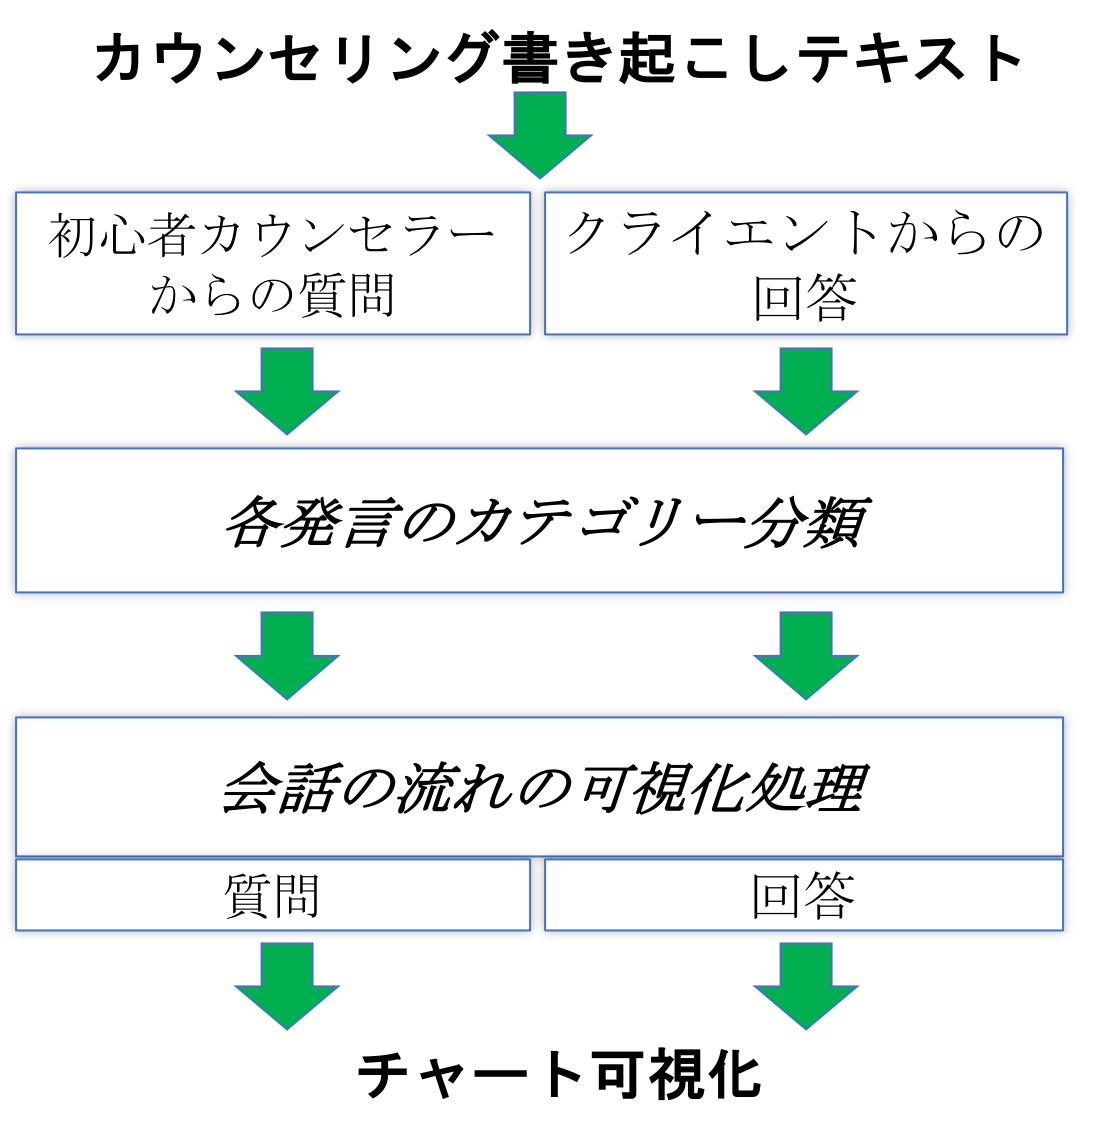
\includegraphics[width=\linewidth]{4_2.png}
  \end{center}
  \caption{会話の流れの視覚的分析システムフロー}
  \label{fig:4_2}
\end{figure}


\subsection{前処理部}

本項では本提案システムの前処理部の実装について述べる.

%クライエントからの提出した話題が,どの領域に関するものか,心理カウンセリングの中でその領域がどのように変わっていくかを分析していくと,その心理カウンセリングプロセスがより明確になると考えられる.時系列に沿って心理カウンセリングの会話の流れを見ることで,最初にクライエントが抱いている問題がどこにあったのか,それに対してカウンセラーからの発話で異なった領域に話題が展開した,というような分析も可能になると考えられる.クライエント側の関心に注意を向けるということが心理カウンセリングの基本であるため,カウンセラー側の関心でクライエントを誘導してしまうことはよくないとされる.そのためのチェックが本提案システムによって可能になることが期待される.もうひとつのタスクとしては,初心者のカウンセラーは「閉じられた質問(Closed-ended Question)」を多用するので,初心者のカウンセラーが「閉じられた質問」だけでなく「開かれた質問(Open-ended Question)」も使いこなせるように熟練カウンセラーが指導する必要がある.%そのチェックも本提案システムによって可能になることが期待される.






% また本提案システムのユースケース図を図
% \ref{fig:use_case_diagram}
% に示す.
% ユースケース図は,システムがどのように機能すべきか,およびその外部環境を表すUMLの図である.
% UMLは,主にオブジェクト指向分析や設計のための,記法の統一がはかられた(Unified)モデリング言語(Modeling Language)である.




% \begin{figure}
%   \begin{center}
%     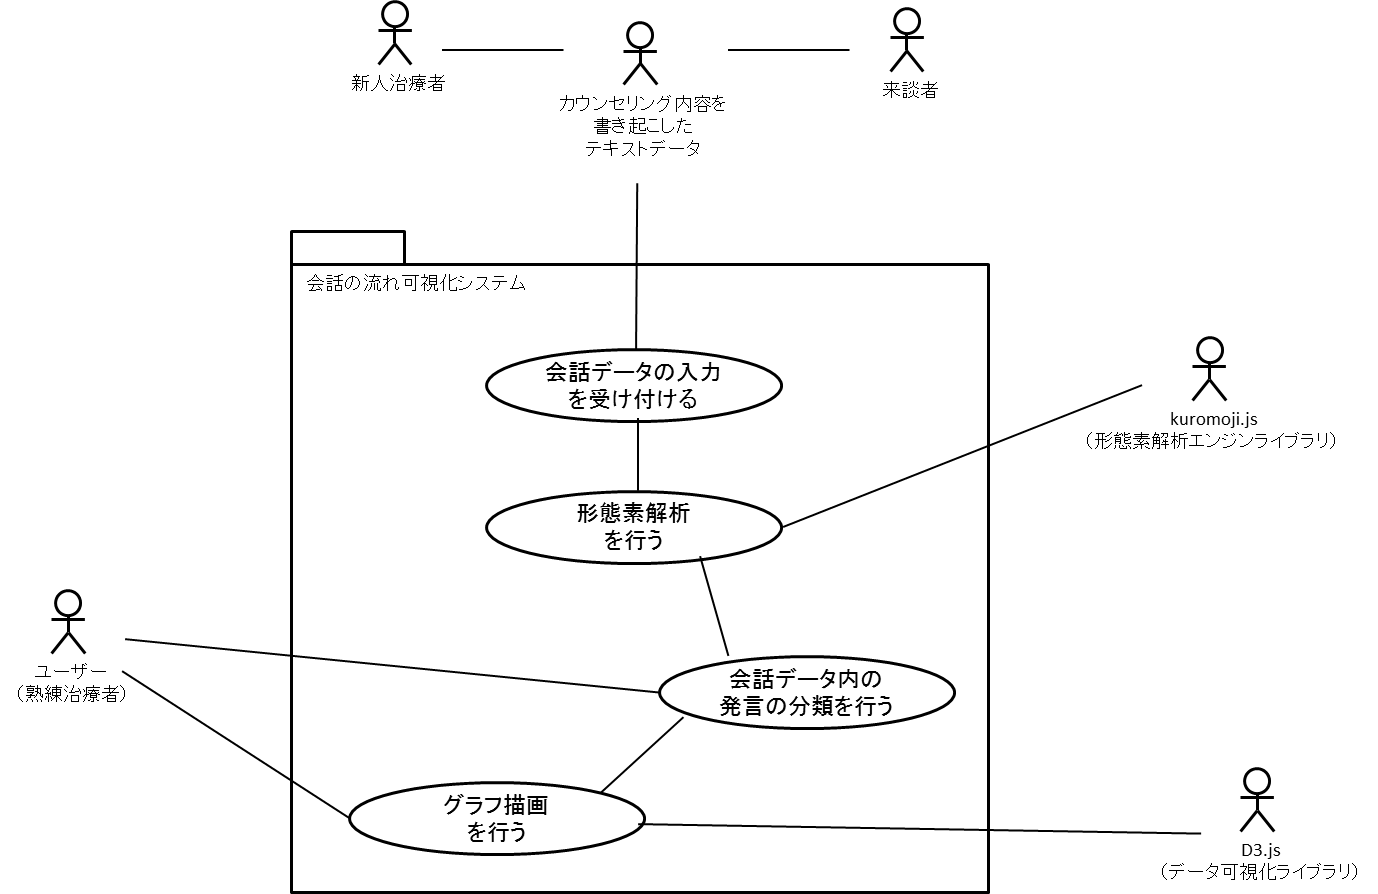
\includegraphics[width=\linewidth]{use_case_diagram.png}
%   \end{center}
%   \caption{会話の流れの視覚的分析システムのユースケース図}
%   \label{fig:use_case_diagram}
% \end{figure}


まず,グラフ描画前のテキストデータ処理について説明する.会話の流れの視覚的分析システムのテキストデータ処理のアクティビティ図を図
\ref{fig:activity}
に示す.%アクティビティ図とはフローグラフに似た図で,いわゆるビジネスロジックにおける手続き的な流れやプログラムの制御フローを表すUMLの図である.
\begin{figure}
  \begin{center}
    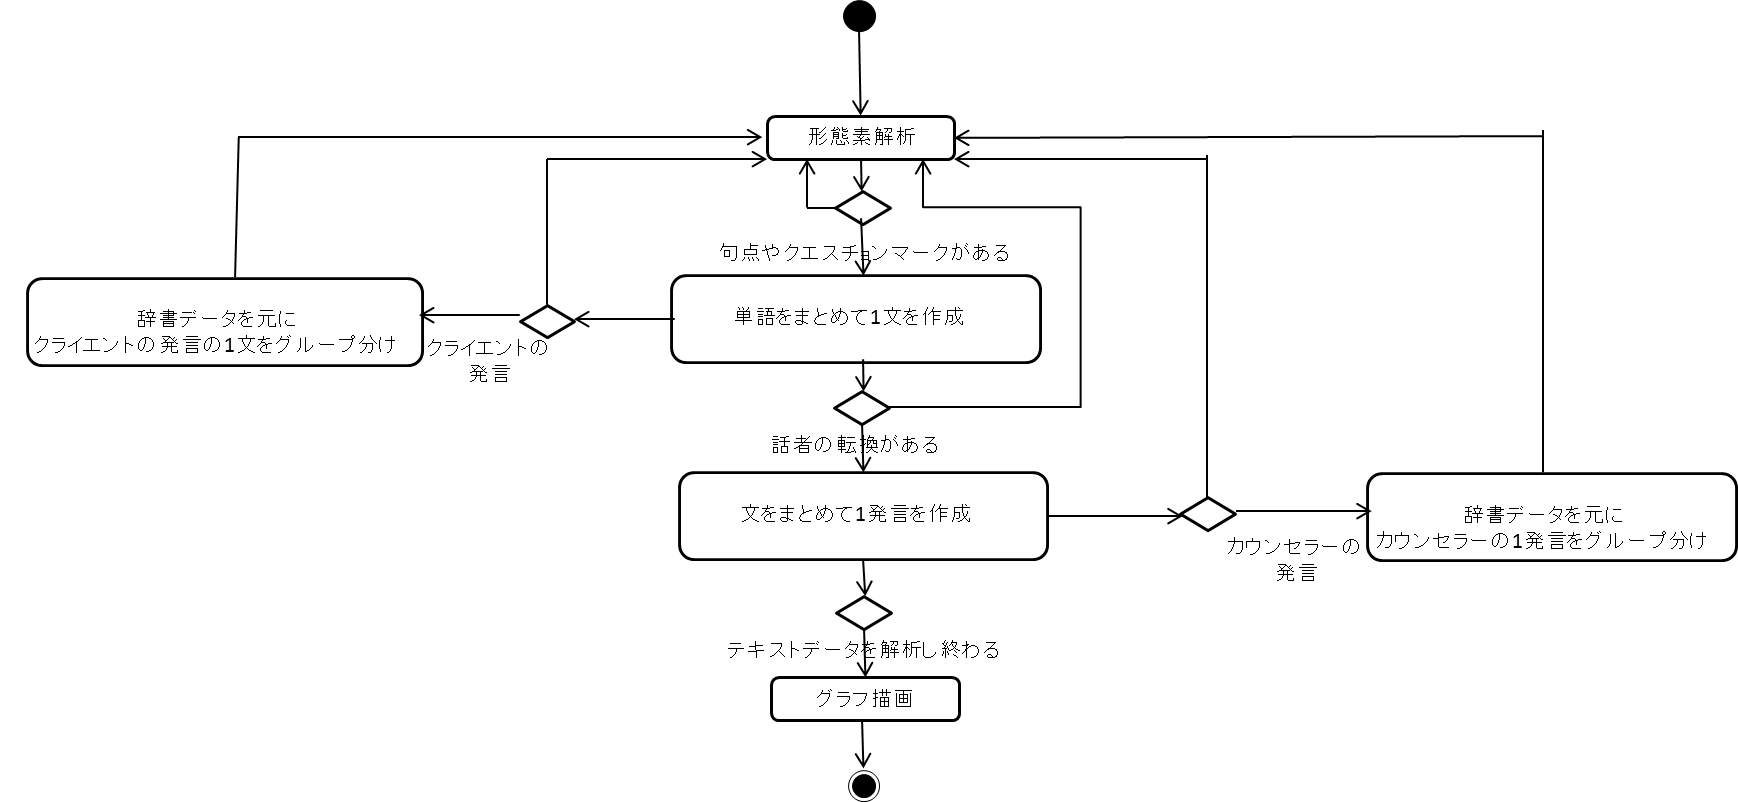
\includegraphics[width=\linewidth]{activity.png}
  \end{center}
  \caption{会話の流れの視覚的分析システムのテキストデータ処理のアクティビティ図}
  \label{fig:activity}
\end{figure}


初めに,Webブラウザ上で各テキストの会話データを読み込んで,テキストを単語ごとに区切る形態素解析を行う.会話データ読み込み前の本提案システムスクリーンショットを図
\ref{fig:yomikomimae2}
に示す.
\begin{figure}
  \begin{center}
    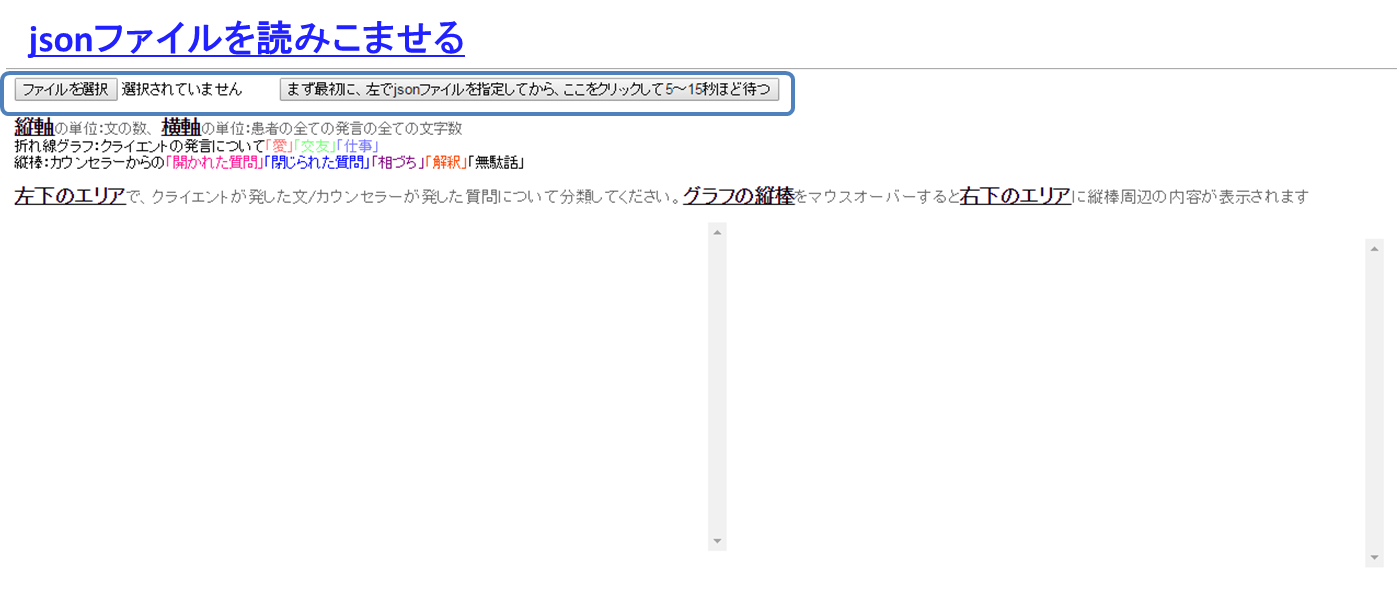
\includegraphics[width=\linewidth]{yomikomimae2.png}
  \end{center}
  \caption{会話データ読み込み前のシステムスクリーンショット}
  \label{fig:yomikomimae2}
\end{figure}

ここで,本提案システム評価で使用する入力データについて説明する.
% 本章の提案システムにおいて,心理カウンセリングを書き起こしたデータを全15個に分けて使用した.以降この15個のデータをそれぞれ,会話データ1,2,3,……,15と呼ぶこととする.
この本論文の実験で用いる対象データには「ヨーガ療法事例検討会」資料から引用したものである.
また,後述する初期グラフ描画がある程度有用なものかを示すために模擬会話データを1個用意した.

形態素解析には,JavaScript言語の形態素解析ライブラリであるkuromoji.js\cite{kuromojijs}を使用した.kuromoji.jsは,Javaで実装されたオープンソースの日本語形態素解析エンジンKuromoji
\cite{kuromoji}
を,JavaScriptに移植したものである.

次に,以下の手順に従って,会話データの分類処理が行われる.

\subsubsection{(1)1文,1発言毎による会話データの分割}%%%%%%%%%%%%%%%%%%%%%%%%%%%%%%%%%%%%%%%
形態素解析された単語群から,句点やクエスチョンマークを終点と定義して1文毎に分割して,テーブルを作成する.さらに,話者の切り替わりを全角コロンで定義し,全角コロンと全角コロンの間の文のカテゴリーを1発言と定義し,発言単位でテーブルを作成する.クライエントの回答の中で,各カテゴリーに属する文に入っていそうな単語を,「愛」「仕事」「交友」「自己」「スピリチュアル」ごとに指定した辞書をつくっておき,発言データの文を構成する単語が指定された単語と一致する場合,この情報を図
\ref{fig:4_2}
の発言のカテゴリー分類に引き渡し,発言カテゴリー分類の初期設定値を計算する.
%この初期選択において,今回は簡単化のため,複数のカテゴリーの可能性をもつ1文に対しては,「愛」の可能性があれば「愛」に,それ以外は「仕事」に分類するようにした.

%%実装

% 前節で説明した要件抽出にもとづいて,本研究では会話の流れ視覚的分析システムの実装を行った.本節では,会話の流れ視覚的分析システムの,可視化する前の処理の部分について説明を行う.


% 臨床的観点からは,三つのカテゴリーに人間の問題を分類するために極めて有効であると考えられる.上記分類手法から,本研究では次項で提案されたシステム,設計および実装するための要件を説明する.

% このセクションでは,提案システムの設計と実装について説明する.図3は,心理カウンセリングでの会話の流れの視覚的分析システムの処理手順を示している.会話の流れの可視化は)1つの心理カウンセリングセッションでの会話の内容を示している.このシステムでは,可視化の前処理として,心理カウンセリングにおける会話のテキストデータのカテゴリー分類が実行される.

% まず,提案システムは,ブラウザ上で各テキストの会話データを読み,言葉にテキストを分離するために形態素解析を行う.形態素解析サブシステム内で使用されたJavaScript言語の形態素解析ライブラリであるkuromoji.js\cite{kuromojijs}は,JavaソースのKuromoji\cite{kuromoji}からJavaScriptに移植されたオープンソース日本語形態素解析エンジンである.

% クライエントの回答は,文の各単語に対応するキーワードとのマッチングにより,各カテゴリーに分類される.このシステムでは,カウンセラーの発言の分類単位は,すなわち,話者が話し始めてから別の話者が話し始めるまでを1発言とし,この1発言をカテゴライズする1単位とした.

% しかし,このカテゴリーの分類手法ではカウンセラーとクライエントによって各発話のテキストデータに適用し,分類結果の精度は,システムに登録されている単語辞書に依存し,分類のための正解率は非常に低いである.そのため,専門家のカウンセラーは,現在のシステムでは,最初の分類結果を確認し,手動で誤分類結果を修正する必要があり,作業負担が大きい.クライエントのそれとは違って,私はセラピストの発話の分類は,文単位が,話し手ターン単位での分類ではないというコメントを得た.






%%%%%%%%%%%%%%%%%
\subsubsection{(2)クライエントの回答の分類}



ここで述べるクライエントの回答に関する分類に関しては,1発言単位ではなく1文単位でカテゴリー分類を行う.その理由は,1発言の中で例えば「愛」から「仕事」へ話題が移る可能性があるからである.

たとえば,「うちの夫は仕事にいくのを嫌がって,毎朝起きてこないんです.
それを見ているだけで腹が立つんです.自分の同僚が同じように仕事に行きたいですが
朝起きなかったという話を聞いても,さほど腹は立ちませんが,夫がそ
うなるのは絶対に許せない」という文章について,熟練カウンセラーは次の通りに分類する.1文は愛のタスク,2文は仕事のタスク,3文は愛のタスクに分類する.%回答カテゴリー一覧を表\ref{table:ansCate}に記す.

% \begin{table}
%   \caption{回答カテゴリー一覧}
%   \label{table:ansCate}
%   \begin{center}
%     %\includegraphics[width=\linewidth]{table2.png}
%     \begin{tabular}{|l|p{7cm}|} \hline
%       愛 & クライエント自身の家族や恋人との関係.家族自身の仕事関係なども含む.
%       \\ \hline
%       交友  & クライエント自身の友人関係.友人自身の仕事関係なども含む
%       \\ \hline
%       仕事 & クライエント自身の勉強・仕事の結果,上司・同僚・部下・取引先・客などとの仕事上の対人関係
%       \\ \hline
%       自己  &  クライエント自身との付き合い・自己存在.セルフタスク・症状などに関すること
%       \\ \hline
%       スピリチュアル & 超越的存在との付き合い
%       \\ \hline
%     \end{tabular}
%   \end{center}
% \end{table}

% \item 仕事のタスク(work task):クライエント自身の勉強・仕事の結果,上司・同僚・部下・取引先・客などとの仕事上の対人関係
% \item 交友のタスク(friendship task):クライエント自身の友人関係.友人自身の仕事関係なども含む
% \item 愛のタスク(love task):クライエント自身の家族や恋人との関係.家族自身の仕事関係なども含む.
% \item 自分自身のタスク(self task):自分自身との付き合い・自己存在
% \item スピリチュアリティのタスク(spiritual task):超越的存在との付き合い\cite{大友秀治2013全人的人間理解を促進するスピリチュアリティ概念に関する一考察}



% ここから得られる要件は,クライエントの回答の分量に応じて,それをはさむカウンセラーの発言の縦棒をグラフ上で変えることであると考えた.

% クライエントの回答に関する分類に関しては,1発言単位ではなく1文単位で「愛」「交友」「仕事」を分類するように変更することが求められる.
% たとえば,「うちの夫は仕事にいくのを嫌がって,毎朝起きてこないんである.
% それを見ているだけで腹が立つんである.自分の同僚が同じように仕事に行きたが
% らなくて朝起きなかったという話を聞いても,さほど腹は立ちないが,夫がそ
% うなるのは絶対に許せない」という文章について,専門家は次の通りに分類する.1文は愛のタスク,2文は仕事のタスク,3文は愛のタスクに分類する.

% 原文から,カウンセラーからクライエントへの質問事項の分類の指標として,クライエントの回答をうながしてクライエント自身も気づいていなかったことを認知させるのが大事であるので,それぞれの発言量の可視化の実装を盛り込むべきであるというコメントを得た.ここから得られる要件は,クライエントの回答の分量に応じて,それをはさむカウンセラーの発言の縦棒をグラフ上で変えることであると考えた.

クライエントの回答に関する分類を行うために次の操作を行った.まず形態素解析された単語群から,句点やクエスチョンマークを終点と定義して1文ずつのテーブルを作成する.さらに,話者の切り替わりを全角コロンで定義し,全角コロンと全角コロンの間の文のカテゴリーを1発言と定義し,発言単位でテーブルを作成する.「クライエントの発言においてこれを含む文はこのカテゴリーに属するだろう」という単語を,「愛」「仕事」「交友」ごとに指定しておき,発言データの文を構成する単語が指定された単語と一致する場合,この情報を図\ref{fig:4_2}の「各発言のカテゴリー分類」に引き渡し,発言データ分類の初期設定値を計算する.

なお,林田ら\cite{hayashidaEn}はこの「愛」「仕事」「交友」の分類について,Yahoo!知恵袋をコーパスとしたSVMでの分類を提案したが,本研究ではその精度を向上させた.詳しくは3.5節で述べる.


\subsubsection{(3)カウンセラーの発言の分類}





%カウンセラーの発言の分類について,まずカウンセラーの発言も,次章で説明する初期分類は適当ではないことがあるので,クライエントからの返答だけでなく,カウンセラーの発言区分けも手動で修正したいというコメントを得た.

カウンセラーの1発言についても,クライエントの回答の1文ごとの分類と同様に,関連する単語をあらかじめ指定しておき,必要情報を図\ref{fig:4_2}の「各発言のカテゴリー分類」に引き渡し,発言データ分類の初期設定値を計算する.カウンセラーの発言分類の中で特に「開かれた質問」「閉じられた質問」は,その質問の次にクライエントのどのような回答(yes/noで応えられるか否か,など)が一意に定まるので,1発言全体についてカテゴリー分類を行う.

% ここで会話データを入力した後のカウンセラーの初期分類状態の分類手法について説明する.今回の実際の会話データ15個のうち,カウンセラーの発言数は398発言あったが,本提案システム要件の質問分類の「相槌」に含まれるべき短文に「そうであるか」というフレーズが41箇所あった.富士通株式会社は質問文判定について特許
% \cite{tokkyo}
% を取得しているが,富士通株式会社の特許技術において行われている「(る)か」という文の終わり方だけで質問判定を行うだけでは,「そうであるか」というフレーズも自動的に「相槌」ではなく「閉じられた質問(Closed-ended Question)」に分類してしまうので不適当である.



% また,質問内容は,前章の要件通り5種類に分類され,後述する縦棒アイコンの色の割り当ては次の通りである.赤色は5W1H「いつ」「どこで」「誰が」「何を」「どのように」「どうした」などで問われるような「開かれた質問(Open-ended Question)」,青色はYes/Noで答えられる,あるいは一言だけで簡単答えられるような「閉じられた質問(Closed-ended Question)」,紫は「相槌」,オレンジはクライエントの問題をカウンセラーがどう「解釈」しているかの確認,黒は「世間話」を表現している.1章で説明した通り,クライエントが何に問題意識を感じているかに対して心理カウンセリングでカウンセラーの関心を傾聴するには,カウンセラーは「閉じられた質問(Closed-ended Question)」よりも「開かれた質問(Open-ended Question)」をしたほうがよいとされている

% まず会話データ入力サブシステムで心理カウンセリングの書き起こしテキストデータを入力し,形態素解析サブシステムに引き渡す.
% 形態素解析サブシステムでは,カウンセラーの1発言についても,クライエントの回答の分類と同様に,関連する単語をあらかじめ指定しておき,必要情報をFig.1の発言データ分類サブシステムに引き渡し,発言データ分類の初期設定値を計算する.

本提案システムにおける,会話データを入力した後のカウンセラーの初期分類状態の分類手法を図
\ref{fig:5_2}
に示す.
\begin{figure}
  \begin{center}
    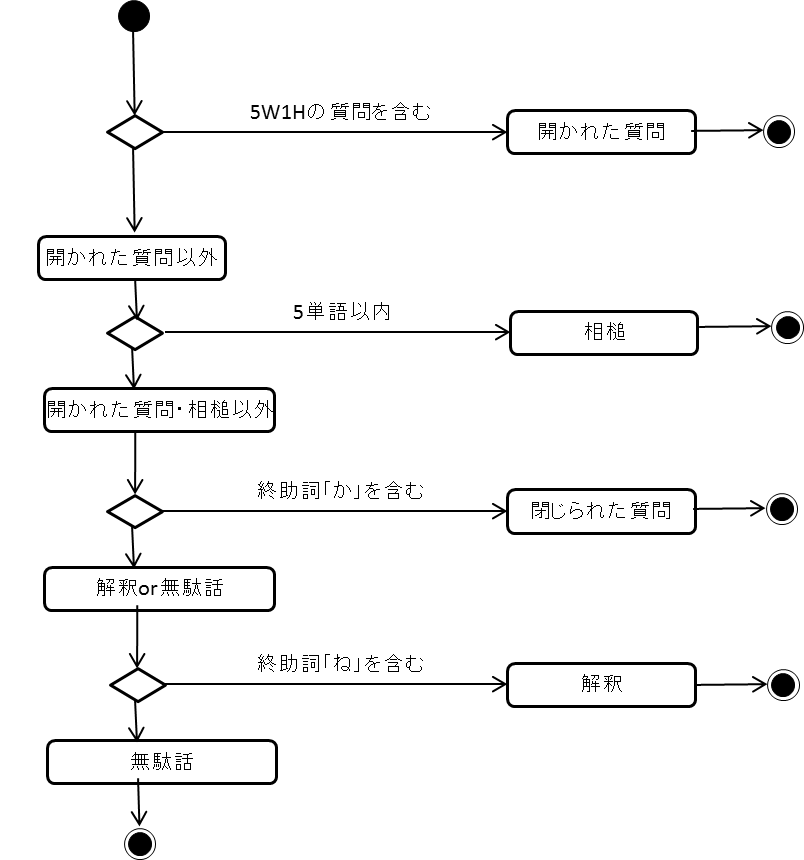
\includegraphics[width=\linewidth]{5_2.png}
  \end{center}
  \caption{カウンセラーの発言の初期分類手法}
  \label{fig:5_2}
\end{figure}
まず「いつ」「どこ」「何」などのいわゆる5W1Hを示す疑問詞をもつ発言を「開かれた質問(Open-ended Question)」に分類する.次に残りの発言のうち,単語数が5個以下のものを「相槌」に分類する.さらに残りの発言のうち終助詞「か」を含む発言を「閉じられた質問(Closed-ended Question)」に分類する.今までの3つに分類されなかったものは「解釈」か「世間話」に分類されるわけだが,終助詞の「ね」を含むものを「解釈」,含まないものを「世間話」とした.



% 一方,クライエントの回答の各1文の分類手法として,ヨーガセラピーが基本としているアドラー心理学の3つのライフタスク7)(「愛」「仕事」「交友」)分類カテゴリーとして用いることにした.
% 会話データを発言データ可視化サブシステムに受け渡し,カウンセラーの発言の分類結果と,クライエントの回答のカテゴリー分類結果を併せて,時間経過に沿った分布変化としてグラフによる可視化表示を行う.

以上の前処理後のデータを会話データ可視化処理部に受け渡し,初心者のカウンセラーの発言のカテゴリー分類結果と,クライエントの回答のカテゴリー分類結果をあわせて,時間経過に沿った分布変化としてグラフを用いた可視化表示を行う.


% システム設計と実装








%\subsection{クライエントの回答に関する分類} %%%%%%%%%%%%%%%%%%%%%%%%%%




%\subsection{カウンセラーの発言に関する分類} %%%%%%%%%%%%%%%%%%%%%%%%

\subsection{会話データの可視化処理部} %%%%% 3.3.2項

%前節では,会話の流れ視覚的分析システムの可視化前の処理の部分の実装について説明を行った.本節では,
次に,前処理後の可視化処理部について説明を行う.


%%可視化結果をゴリゴリ説明


%のスライダーを動かすことによって,本研究ではどのような文を時系列に沿ってどのような文に,例えば,人間関係からグラフを表示した.また,図2に示すように,それが可能な,対応する動詞の文章を表示することによって,本研究では,矢印は,図手段として,元のどのテキストを知ることができる.

本研究では,会話データの可視化処理の実装にD3.js\cite{vand3}を用いた.D3.jsはウェブブラウザ上で動的なコンテンツを可視化するためのJavaScriptのライブラリであり,ニューヨーク・タイムズ紙サイト内のグラフ描画などに用いられている.




\subsubsection{グラフを用いた会話データの可視化}
本提案システムではカウンセラーからの発言カテゴリーと,クライエントの回答一文毎に対して「愛」「仕事」「交友」「自己」「スピリチュアル」にカテゴリー分類された結果を,時間経過に沿った分布変化として可視化する.また,各会話データに対して,積み重ね折れ線グラフと帯グラフを用いた可視化手法を実装した.
% グラフ描画の際に,会話データを発言データ可視化サブシステムに受け渡す.このサブシステムでは,データ可視化ライブラリD3.js
% \cite{bostock2012d3}
% を使用した.模擬会話データを入力し,後述する
積み重ね折れ線グラフを出力した際の結果を図
\ref{fig:6_1}
に示す.
% また模擬会話データの原文と,模擬会話データ時の初期自動分類結果を表
% \ref{table:book1}
% に示す.
\begin{figure}
  \begin{center}
    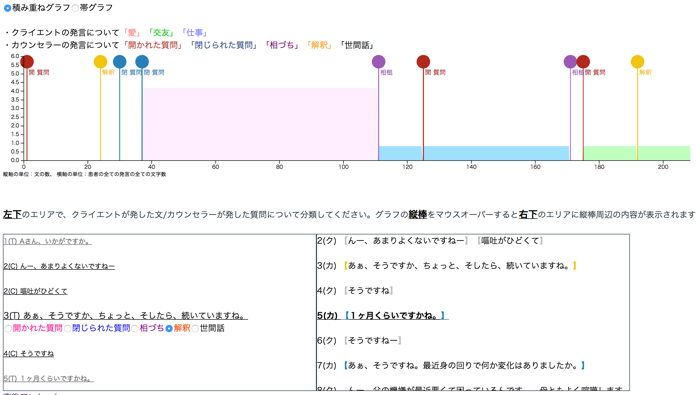
\includegraphics[width=\linewidth]{6_1.png}
  \end{center}
  \caption{模擬会話データでのシステム出力結果(積み重ね折れ線グラフ,縦軸:文の数,横軸:クライエントの全ての発言の累計文字数)}
  \label{fig:6_1}
\end{figure}

% \begin{table}
%   \caption{模擬会話データでの初期表示用自動分類結果}
%   \label{table:book1}
%   \begin{center}
%     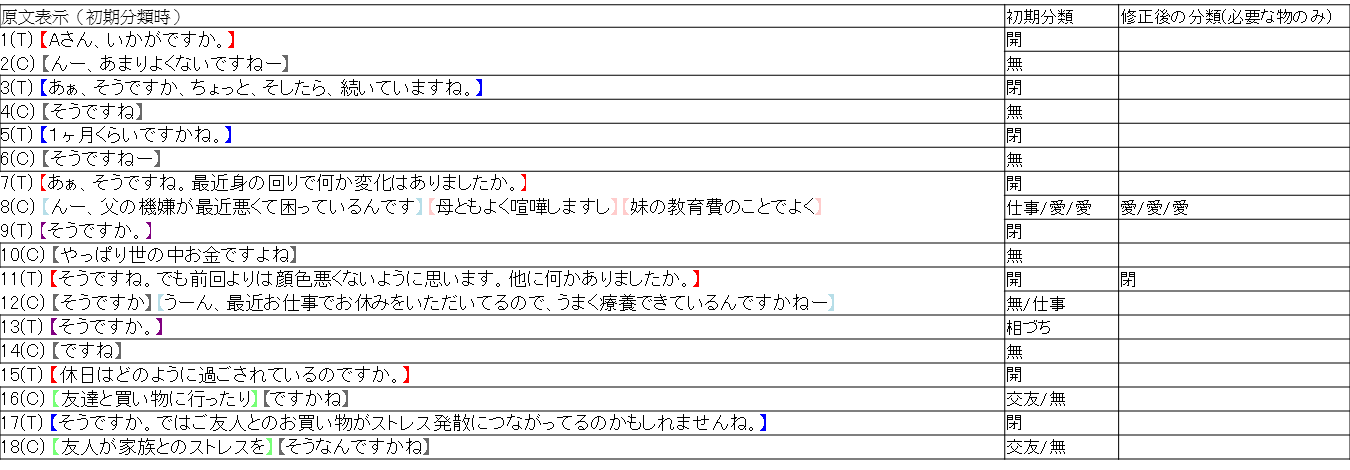
\includegraphics[width=\linewidth]{book1.png}
%   \end{center}
% \end{table}



% まず,提案した,積み重ね折れ線グラフと縦棒を用いた可視化について説明する.
図
\ref{fig:6_1}
において,まず積み重ね折れ線グラフはクライエントの1回の発言の中での,アドラー心理学の各カテゴリーの分布を可視化している.ただし1回の発言は,話者の交代を発言の区切れ目とする.この積み重ね折れ線グラフにおいて薄い水色は「仕事関係」,ピンク色は「愛(恋愛・愛関係)」,薄い緑色は「交友(友人関係)」,黄色は「自己」,紫は「スピリチュアル」に密接に関係する単語を含む文の分布を表している.

横軸は時間軸を表現している.ただし対象データである書き起こしテキストデータからは実際の経過秒数は読み取れないので,読み込ませたデータ内におけるクライエントの回答量の累計の文字数を横軸,つまり時間軸とした.後述するカウンセラーの発言を表現する縦棒はこの時間軸にそって出現する.
% カウンセラーとクライエントの回答の入れ替わりがわかりやすいように,積み重ね折れ線グラフがクライエントの回答のカテゴリー分布をちょうど表しているのは便宜上発言部分の中央部分になっている.

縦軸は発言中の1文の数のうち,どのカテゴリーに何文入っているかという文の数を表している.

%ここで会話データを入力した後のクライエントの回答の各1文の初期分類状態の分類手法について説明する.
%まず,あらかじめこちらで
%次に,各単語群を含むクライエントの回答の1文をカテゴリー分けをしていった.


%Ericら\cite{taskdriven}は,分けたトピックの時間分布を上下の非対称積み重ね折れ線グラフによって可視化した.一方
本研究では,カウンセラーとクライエントの会話において,クライエントは文ごとに,カウンセラーは発言ごとに描画を行いたい,かつ選択肢表示のためにグラフを省スペースしたいという観点から,カウンセラーの発言を横軸より下に折れ線グラフとして描画するのではなく,クライエントの回答のカテゴリー分布を示す積み重ね折れ線グラフに重ねて縦棒として表示するようにした.こうすることによって,クライエントとカウンセラーの発言が交互に描画されるので,クライエントとカウンセラーの発言の関連性がわかりやすくなった.

積み重ね折れ線グラフに重なっている縦棒は,カウンセラーの発言内容の形態を示す.縦棒の色分けは,赤が「開かれた質問」,青が「閉じられた質問」,オレンジが「解釈や助言」,紫は「相槌」,黒が「世間話」を表す.



% \subsubsection{帯グラフを用いた可視化}


さらに,本研究では本提案システムの新たな可視化手法として帯グラフを提案する.この帯グラフによる可視化結果を図\ref{fig:obi}に示す.

図\ref{fig:6_1}の積み重ね折れ線グラフ同様,横軸は時間軸を表す.2本の帯グラフのうち,上側はカウンセラーの発言,下側はクライエントの回答を表す.初心者のカウンセラーの発言とクライエントの回答の各分類カテゴリーおよび色分けについては,それぞれ積み重ね折れ線グラフにおける積み重ね折れ線と縦棒の場合と同様である.

積み重ね折れ線グラフはカウンセラーの発言を縦棒のみで表示しているのに対し,帯グラフはクライエントの回答だけでなくカウンセラーの発言も文量情報を持った表示をしている.そのため,初心者のカウンセラーの発言とクライエントの回答の帯グラフの各色分けされた区間内の長さは,それぞれの発言の長さを表している.対象データである書き起こしテキストデータからは実際の経過秒数は読み取れないので,読み込ませたデータ内における初心者のカウンセラーとクライエント2人の発言量の累計の文字数を横軸とした.

\begin{figure}
  \begin{center}
    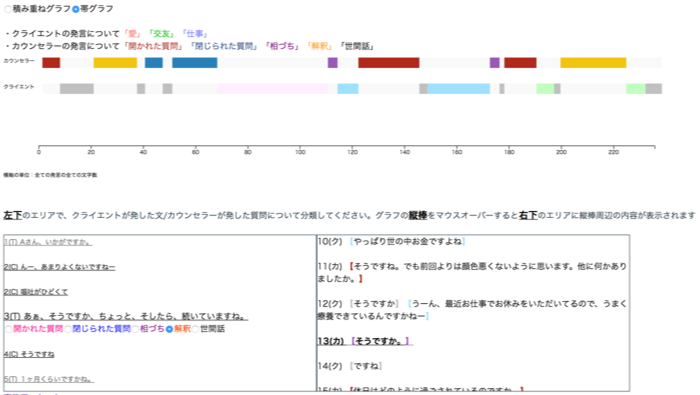
\includegraphics[width=\linewidth]{obi.png}
  \end{center}
  \caption{模擬会話データでのシステム出力結果(帯グラフ,横軸:クライエントとカウンセラーの全ての発言の累計文字数)}
  \label{fig:obi}
\end{figure}

\subsubsection{発言分類手動修正機能}
積み重ね折れ線グラフが描画された後に,グラフ左下のラジオボタンエリアにて,クライエントの回答の各1文およびカウンセラーの各1発言において,分類を変えると即時にグラフ描画に変更が適用されるようにした.この手動変更した結果は,LocalStorageを用いてユーザーの使った各ブラウザ上に保存され,CSV出力/入力によって他ユーザーに引き継ぎ可能である.
%本ラジオボタンエリアがみたした要件については,付録にて記述する.

%\section{要件抽出}

\subsubsection{原文表示機能}

どこがどの発言を表しているかわからないという問題に対しては,両グラフのそれぞれ初心者のカウンセラーの発言やクライエントの回答を表す箇所にマウスカーソルをあわせることによって,グラフ右下に周辺の発言を表示する機能を追加することで解決を図った.見やすさのため,グラフの色に対応した文字色ではなく黒い文字で各発言を表示し,それをグラフと対応した色の隅付き括弧【】で囲うようにした.


%\section{実装}

%%修論からパクってくる


%
% \subsection{ケーススタディ}
%
% 前節までで,本提案システムの前処理手順および可視化手法と可視化結果について説明した.本節では本提案システムにもとづいたユースケースについて説明する.



\section{システム評価}%%%%%%%%%%%%%%%%%%%%%%%%%%% 3.4



% 前節までは,会話の流れ視覚的分析システムの実装およびケーススタディについて説明を行った.
本節では,心理カウンセリングの会話の流れ視覚的分析システムにおける会話データの可視化手法の比較評価,および現場のカウンセラーによる本提案システムの有効性に関する評価を行う.%を用いて「」という仮説を検証するために行ったユーザ評価の目的・手法・結果・考察についてのべる.% カウンセラー習熟度評価支援システムは,主に,
%
% %%ユーザエバリュエーションをゴリゴリ説明
%
%
%
%
% 専門カウンセラーが,彼は「私はBが私の意志に従うことをしたい」という考えが消えていることが分かったと説明した.
%
% 自己閉じタスクが増加した.認知の補正の進行は,することができた 量変更することによって確認 矢印の(複数心理カウンセリングの全体図)をし,元のテキスト表示で品質を確認. 本研究では,我々の提案文字グラフの可視化は,カウンセラーは見つけることができることを検討してください のいくつかの種類がことを ,クライエントの 認知の修正作られた.

% \subsection{シグマ値法}







\subsection{会話データの可視化手法の比較評価}
積み重ね折れ線グラフの形状と帯グラフの形状との比較を行った.前節で説明した会話の流れの視覚的分析システムを,3名の熟練カウンセラーに評価者として実際に使用してもらうことで,会話データの可視化手法として実装した積み重ね折れ線グラフと帯グラフの比較評価を行った.
評価に参加していただいた熟練カウンセラーの平均年齢は55歳,平均臨床歴は29年である.

本比較評価は,「初心者のカウンセラーの関心がクライエントが抱いている問題にどの程度傾聴されているか」について,積み重ね折れ線グラフと帯グラフのどちらがわかりやすく可視化出来ているかを検証する.評価手法として,評価者である熟練カウンセラーは,積み重ね折れ線グラフ,帯グラフによって表示されているそれぞれの可視化結果に対して,時系列に沿ってマウスカーソルを合わせることでで心理カウンセリングの会話原文と併せて参照しながら,心理カウンセリングの流れを一通り確認作業を行う.作業が終了したら,下記に示すアンケート回答による比較評価を行った.

\subsubsection{(1)6段階評価による結果}

本項で説明する比較評価の目的は,「初心者のカウンセラーの関心がクライエントが抱いている問題にどの程度傾聴されているか」が,積み重ね折れ線グラフでの評価よりも,本グラフの帯グラフ可視化モードの方がわかりやすい,という仮説の検証である.まず評価者は,積み重ねグラフ,帯グラフそれぞれについて,あらかじめ表示されている可視化結果に対して,時系列に沿ってマウスカーソルを合わせることで,心理カウンセリングの流れを一通り確認する.

表\ref{table:keijouAnketo}に示す6段階評価による質問項目,および各質問に対する選択肢とその配点に基づいたアンケート質問に対する回答を行う.表\ref{table:keijouAnketo}の各質問項目は,積み重ね折れ線グラフ,帯グラフそれぞれに対して行った.

%6段階評価によるアンケート質問に回答を行う.6段階評価のアンケートの質問項目,および各質問に対する選択肢とその配点を表\ref{table:keijouAnketo}に示す.

積み重ね折れ線グラフ,帯グラフについて,各質問項目に対する6段階評価の平均値の結果を図\ref{fig:keijouAnketo}に示す.図\ref{fig:keijouAnketo}の結果より,全ての項目において,積み重ね折れ線グラフより帯グラフの方が優れていることがわかった.

\begin{table}
  \caption{可視化手法比較アンケートにおける6段階評価質問}
  \label{table:keijouAnketo}
  \begin{center}
    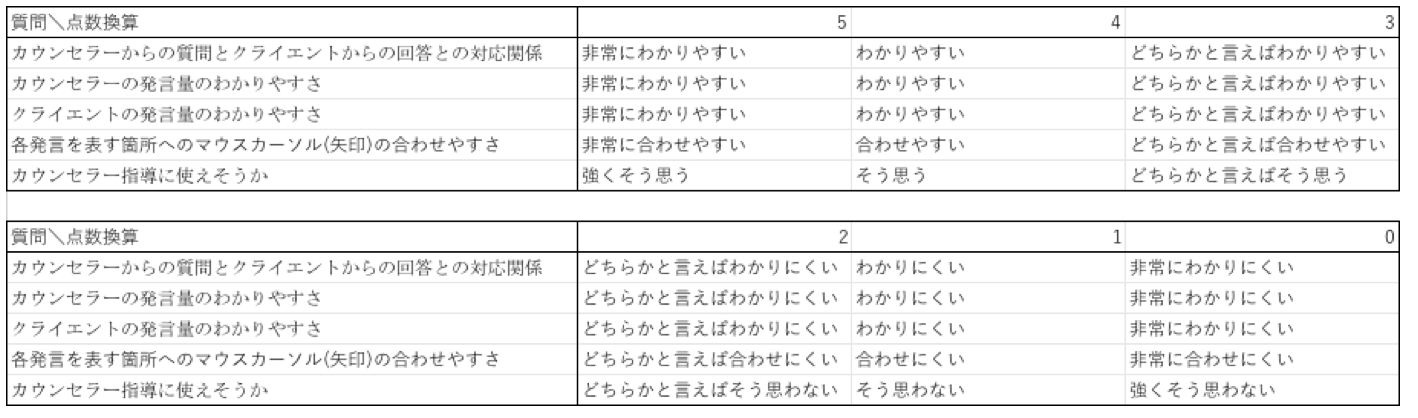
\includegraphics[clip,width=13.0cm]{point.png}
    % \begin{tabular}{|l|p{7cm}|} \hline
    % Work task & Impermanent human relationship \\ \hline
    % Friendship task  & Permanent, and do not fate together human relationship \\ \hline
    % Love or Family task & Fate together human relationship \\ \hline
    % \end{tabular}
  \end{center}
\end{table}

\begin{figure}
  \begin{center}
    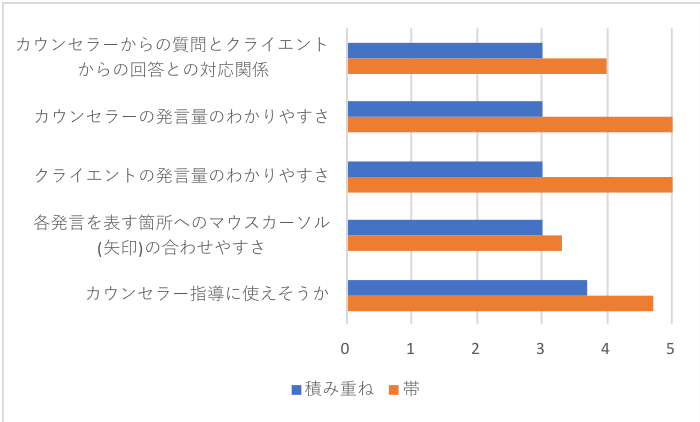
\includegraphics[width=\linewidth]{keijouAnketo.png}
  \end{center}
  \caption{可視化手法比較実験の6段階評価の平均値}
  \label{fig:keijouAnketo}
\end{figure}

%%有意差,相関関係

\subsubsection{(2)自由記述のアンケート}

次に本評価では,以下のQ1〜Q5に記す自由記述の質問アンケートを行った.

\begin{enumerate}
    \renewcommand{\labelenumi}{Q\arabic{enumi}}
  \item 帯グラフを見て,初心者のカウンセラーに対してどのような指導ができるでしょうか
  \item グラフについて,その他全体的に何かご意見があれば,ご回答ください
  \item このシステム全体を用いて,初心者のカウンセラーに対して指導できそうなことがあれば,ご回答ください
  \item 原文表示機能について何かご意見があれば,ご回答ください
  \item このシステムについて,何か他に欲しい機能があれば,ご回答ください
\end{enumerate}

以下に各質問に対する回答結果を示す.

Q1に対しては,
\begin{itemize}

  \item 一回の心理カウンセリング全体を俯瞰し大まかな心理カウンセリングの流れを指導
  \item クライエントとカウンセラーが時系列で対比しながら見ることができるので,一回の面接での流れ,例えば,前半はクライエントに多く喋ってもらっていたのが,後半ではカウンセラーが喋っていたとか,解釈の時に発言量が多いとかが指導できるように思った
\end{itemize}
といった回答が得られた.これより,全体を俯瞰して発言量の分布の変化を基に初心者のカウンセラーに対して,様々な指摘を行えることが考えられる.
Q2に対しては「帯グラフで,それぞれの発言内容の語数や時間が表示されれば,さらに便利かなと思った」という回答が得られた.
Q3に対しては

\begin{itemize}

  \item カウンセラーの発言のチェックとクライエントが抱いている問題に関心を向けているかのチェック」「一回の心理カウンセリングでカウンセラーとクライエントがどのような作業を協力して行っているのか理解を深めること,心理カウンセリングが成立するためにはカウンセラーとクライエントの間で相談的人間関係が構築できていることが前提となることを理解するのに役立つ
  \item 心理カウンセリングがこのように可視化されることだけでも,とても有意義だ
  \item この結果をもとに,心理カウンセリングを再構築するための材料としても使える
\end{itemize}
といった回答が得られた.
Q4に対しては「カウンセラー,クライエントがどこでどんな発言をしているのか確認するのに役に立つと思った」という回答が得られた.

以上の結果から,積み重ね折れ線グラフよりも帯グラフの方が,初心者のカウンセラー指導に優れていると結論づけられる.また全体として,本提案システムが初心者のカウンセラーに対する指導を行うために,会話の流れが適切に可視化されていることが,複数名の熟練カウンセラーの発言によって結論づけられると考える.

Q5に対しては

\begin{itemize}

  \item カウンセラー,クライエントの回答を音声で確認できる機能,心理カウンセリング中のクライエントの身体の動きの変化(心理カウンセリング開始から本題にはいるまで〈相談的人間関係構築がなされているかどうか確認のため〉また特にカウンセラーが解釈投与した直後のクライエントの身体の動き〈解釈投与に対してクライエントがどのような認識反射をおこなっているのかを確認するため〉)についても記されていると便利だと思う
  \item 複数の内容が入った文について,うまく分類できればもっと便利
  \item 内容分類項目のアレンジ機能(追加,修正)
\end{itemize}
といった回答が得られた.
以上の回答から,本提案システムのユーザービリティの改善や機能追加についてさらなる検討を行う必要があり,今後の課題とされる.



\subsection{システムの有用性に関する評価と考察}%%%%%%%%%%%%%%%%%%%%%%%%%%%%%%%%%%%%%%%%%%%%%%%%%%%%%%%%%%%%%%%

%%コメントでゴリゴリ稼げる


前項では,積み重ね折れ線グラフよりも,帯グラフの方が,「クライエントの抱える問題に対して初心者のカウンセラーの関心がどの程度傾聴されているか」の分析を支援する上でより適切な可視化手法であることが分かった.実際の心理カウンセリング内容の原文を用いて,図\ref{fig:pdf}に示す実際の心理カウンセリングの事例検討会に近いスタイルフォーマットの原文のみを読んだ場合と,本研究で提案した帯グラフを用いた「カウンセリングの会話の流れの視覚的分析システム」を用いた場合で同じ作業を行い,比較を行うことで,本提案システムの有効性について評価を行う.また本評価では,前項で説明したユーザーの評価結果を基づいて,会話データの可視化結果として帯グラフを用いる.

\begin{figure}
  \begin{center}
    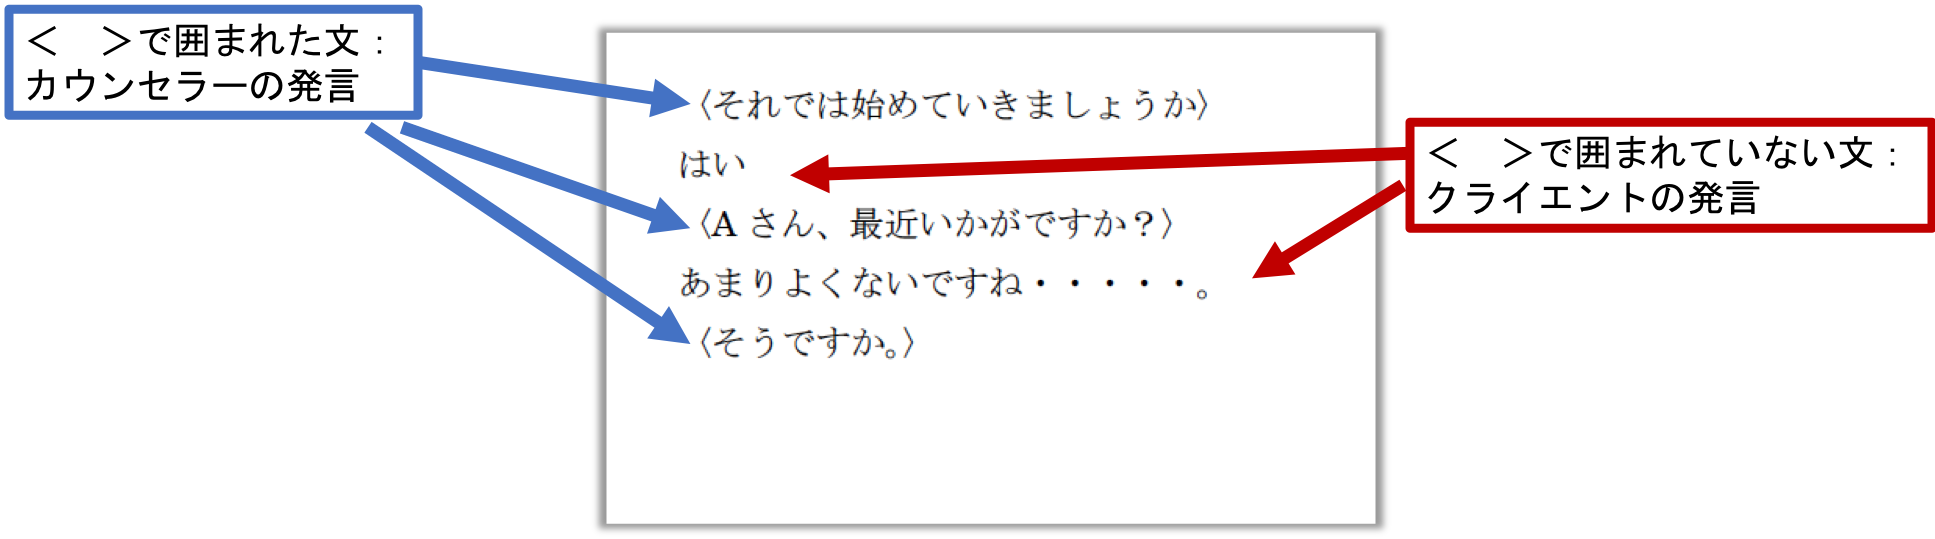
\includegraphics[width=\linewidth]{pdf.png}
  \end{center}
  \caption{実際の心理カウンセリングの事例検討会に近いスタイルフォーマットの例}
  \label{fig:pdf}
\end{figure}

% 本項で説明する比較評価の目的は,「初心者のカウンセラーの関心がクライエントが抱いている問題にどの程度傾聴されているか」が,今日行われている原文を読むだけでの評価よりも,本グラフの帯グラフ可視化モードの方がわかりやすい,という仮説の検証である.会話の流れの視覚的分析システムを,5名のカウンセラーに評価者として実際に使用してもらうことで,システム評価を行った.

本評価では,5名のカウンセラーに評価者として参加してもらった.

% まず
% \begin{itemize}
%   \item 本研究では熟練カウンセラーが初心者のカウンセラーの心理カウンセリング内容の指導や分析を支援するために,「カウンセリングの会話の流れの視覚的分析システム」を実装した
%   \item 本提案システムは,初心者のカウンセラーの発言とクライエントの回答の内容をそれぞれカテゴリー分類して,その結果を時間経過に沿ったカテゴリーの分布変化として可視化表示した
% \end{itemize}
% ことを説明した.その後,


\begin{enumerate}

  \item 事前アンケート
  \item 作業の注意事項
  \item 作業説明
  \begin{enumerate}

    \item 作業1(逐語録を読んでの評価)→ 作業後アンケートのご回答
    \item 作業2(提案システムを使っての評価)→ 作業後アンケートのご回答
  \end{enumerate}
\end{enumerate}
の流れで評価を行った.作業内容として評価者は,
\begin{enumerate}

  \item 心理カウンセリングの原文のみを読む作業
  \item 帯グラフで表示されている可視化結果に対して,時系列に沿ってマウスカーソルを合わせることで心理カウンセリングの会話原文と併せて参照しながら,心理カウンセリングの流れを一通り確認する作業
\end{enumerate}
の2つの作業を行った.作業が終了したら,下記に示すアンケート回答による比較評価を行った.





\subsubsection{(1)6段階評価のアンケート}

表\ref{table:genbunAnke}に示す6段階評価による評価項目,および各質問に対する選択肢に基づいたアンケート質問に対して,評価者が回答を行う.表\ref{table:genbunAnke}の各質問項目は,作業1,作業2それぞれに対して行った.各質問項目に対する6段階評価の結果を図\ref{fig:q1},\ref{fig:q2},\ref{fig:q3}に示す.

\begin{table}
  \caption{有効性検証実験の6段階評価アンケート項目}
  \label{table:genbunAnke}
  \begin{center}
    %\includegraphics[width=\linewidth]{table2.png}
    \begin{tabular}{|p{4cm}|p{4cm}|p{4cm}|} \hline
      Q1:今回取り扱った心理カウンセリングの会話データを,作業1,2の手法で閲覧することで,「初心者のカウンセラーがどの程度開かれた質問を使用しているか」が,どの程度わかりやすかったですか? & Q2:今回取り扱った心理カウンセリングの会話データを作業1,2の手法で閲覧することで,「カウンセラー側が自分の意見を言いたがる程度」が,どの程度わかりやすく感じたでしょうか? & Q3:作業1,2の閲覧手法は初心者のカウンセラー指導に使えると,どの程度思いましたか?
      \\ \hline
       非常にわかりやすい & 非常にわかりやすい & 強くそう思う
      \\ \hline
      わかりやすい & わかりやすい & そう思う
      \\ \hline
      どちらかと言えばわかりやすい & どちらかと言えばわかりやすい & どちらかと言えばそう思う
      \\ \hline
      どちらかと言えばわかりにくい & どちらかと言えばわかりにくい & どちらかと言えばそう思わない
      \\ \hline
      わかりにくい & わかりにくい & そう思わない
      \\ \hline
      非常にわかりにくい & 非常にわかりにくい & 強くそう思わない
      \\ \hline
    \end{tabular}
  \end{center}
\end{table}

\begin{figure}
  \begin{center}
    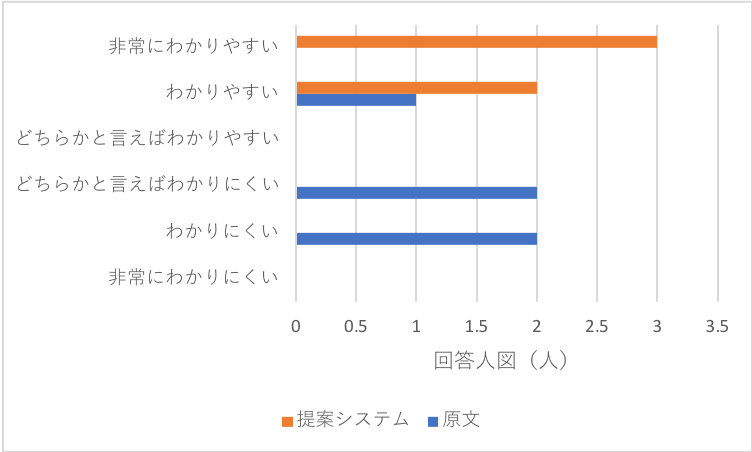
\includegraphics[width=\linewidth]{q1.png}
  \end{center}
  \caption{Q1:今回取り扱った心理カウンセリングの会話データを,作業1,2の手法で閲覧することで,「初心者のカウンセラーがどの程度開かれた質問を使用しているか」が,どの程度わかりやすかったですか?}
  \label{fig:q1}
\end{figure}

\begin{figure}
  \begin{center}
    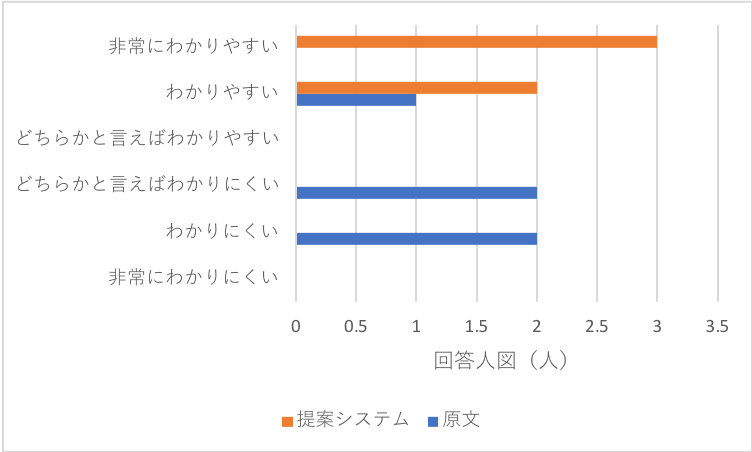
\includegraphics[width=\linewidth]{q1.png}
  \end{center}
  \caption{Q2:今回取り扱った心理カウンセリングの会話データを作業1,2の手法で閲覧することで,「カウンセラー側が自分の意見を言いたがる程度」が,どの程度わかりやすく感じたでしょうか?(Q1と同一の結果となった)}
  \label{fig:q2}
\end{figure}

\begin{figure}
  \begin{center}
    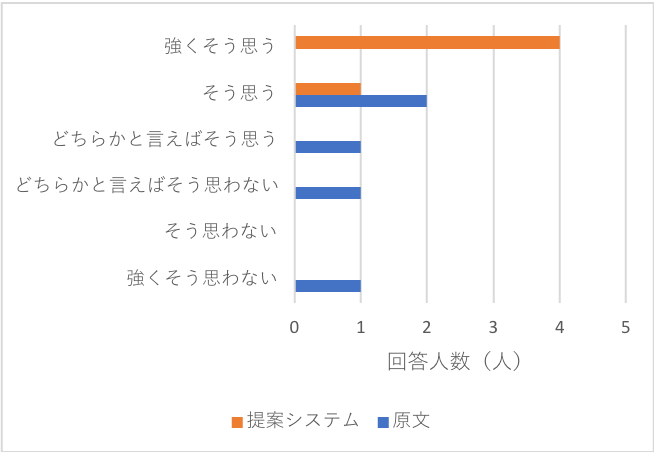
\includegraphics[width=\linewidth]{q3.png}
  \end{center}
  \caption{Q3:作業1,2の閲覧手法は初心者のカウンセラー指導に使えると,どの程度思いましたか?}
  \label{fig:q3}
\end{figure}

ここで作業1(逐語録を読んでの評価)と作業2(提案システムを使っての評価)のそれぞれに対する回答間に有意差があるか調べる.順序尺度でとった今回のアンケートについて,各選択肢間の間隔の差は心理的に等間隔ではない可能性がある.そのため付録Aで詳述するシグマ値法を用いて重み付けのある間隔尺度のカテゴリー得点に換算することで,選択肢間の心理的な距離を反映した点数の重み付けを行った.
各質問に対する回答においてシグマ値法で点数を算出した結果を表\ref{table:sigma}, \ref{table:sigma2}に示す.


\begin{table}
  \caption{Q1,2に対する回答においてシグマ値法で算出した点数}
  \label{table:sigma}
  \begin{center}
    %     \includegraphics[width=\linewidth]{table1.png}
    \begin{tabular}{|l|r|} \hline
      非常にわかりやすい & 1.159 \\ \hline
      わかりやすい  & 0.129 \\ \hline
      どちらかと言えばわかりやすい & なし \\ \hline
      どちらかと言えばわかりにくい & -0.532 \\ \hline
      わかりにくい  & -1.400 \\ \hline
      非常にわかりにくい & なし \\ \hline
    \end{tabular}
  \end{center}
\end{table}

\begin{table}
  \caption{Q3に対する回答においてシグマ値法で算出した点数}
  \label{table:sigma2}
  \begin{center}
    %     \includegraphics[width=\linewidth]{table1.png}
    \begin{tabular}{|l|r|} \hline
      強くそう思う & 0.966 \\ \hline
      そう思う  & 0.129 \\ \hline
      どちらかと言えばそう思う & -0.677 \\ \hline
      どちらかと言えばそう思わない & -1.045 \\ \hline
      そう思わない  & なし \\ \hline
      強くそう思わない & -1.755 \\ \hline
    \end{tabular}
  \end{center}
\end{table}


\begin{enumerate}
  \renewcommand{\labelenumi}{Q\arabic{enumi}}

  \item 今回取り扱った心理カウンセリングの会話データを,作業1,2の手法で閲覧することで,「初心者のカウンセラーがどの程度開かれた質問を使用しているか」が,どの程度わかりやすかったですか?
  \item 今回取り扱った心理カウンセリングの会話データを作業1,2の手法で閲覧することで,「カウンセラー側が自分の意見を言いたがる程度」が,どの程度わかりやすく感じたでしょうか?
  \item 作業1,2の閲覧手法は初心者のカウンセラー指導に使えると,どの程度思いましたか?
\end{enumerate}
の質問に対する回答において,作業1(逐語録を読む)と作業2(提案システムを使う)に対する回答間について,
その点数を用いてt検定を行った結果,Q1,2に関してはt=0.0432,Q3に関してはt=0.0309となり,有意差が見られた.
これらの結果から,
「逐語録を読むだけ」より「本提案システムを用いる手法」の方が,
\begin{itemize}
  \item 「初心者のカウンセラーがどの程度開かれた質問を使用しているか」がわかりやすい
  \item 「カウンセラー側が自分の意見を言いたがる程度」がわかりやすい
  \item 初心者のカウンセラー指導に使える
\end{itemize}
という知見が得られた.


%%有意差,相関関係
\subsubsection{(2)自由記述による評価結果}
%
%
% さらに本評価では,以下の(1)~(5)に記す自由記述の質問を行った.
%
%
%
% \begin{enumerate}
%   \item 帯グラフを見て,カウンセラーに対してどのような指導ができるでしょうか
%   \item グラフについて,その他全体的に何かご意見があれば,ご回答ください
%   \item このシステム全体を用いて,カウンセラーに対して指導できそうなことがあれば,ご回答ください
%   \item 原文表示機能について何かご意見があれば,ご回答ください
%   \item このシステムについて,何か他に欲しい機能があれば,ご回答ください
% \end{enumerate}




%%コメントでページ数稼げる


以下のような熟練カウンセラーからのコメントを得た.ここでは熟練カウンセラーからのコメントから得た考察について述べる.尚,「作業1」が逐語録(原文)のみを読む作業,「作業2」が提案システムを使う作業,「CL」とはクライエントのことである.
% \begin{itemize}
%   \item 作業2について・・・大変ユニークなシステムで,開かれた質問量とその後のCLの語りの割合がとても見やすかったです.また,原文表示機能とのリンクが,素晴らしいと思います.このままでも,十分に利用したいと思える機能ですが,出来が良いだけに欲が出ました.以下の要望があります.部分的な事はわかりましたが,全体の流れの中で最終的にどの程度の割合(何%)になっているのかまで分かると,更に詳細に自己分析する手助けになると思います.また,何ケースも経験を重ねていく中で,質問がうまくなると開かれた質問の%が増えて行き,それに伴いCLの語りの%が増えるような現象がみられると,なお面白い研究だと思えます.
%
%   \item 今回の例では,理想像の母親に対しての,確認の作業を閉じられた質問で展開し,その後のCLの回答を踏まえて,解釈を提示していき,理想の母親に近づく為の考えを導いていく為に,開かれた質問が展開されてきていると感じました.その流れが,作業1よりも,作業2の方で,明確に理解出来ました.
%   \item 原文だけではイメージしにくい5つの分類を明快に色分けされ色ごとに会話の長さが直線表示されたことで解釈等で結構喋っていることがわかりました.また世間話の項目もある事で,振り返りの際に積極的に無駄をなくすことにつながると思います.それらが質問で投げかける言葉の選択や,心理カウンセリングの質を上げる事になると思いました.
%
%   \item 言葉数が多いということだけでも意見を言いたがっていることがわかる.説明的であり,クライエントに自分の考えを一方的に押し付けている.クライエントの発する言葉をきちんと捉え,その言葉の意味を聞いていくというのではなく,カウンセラー側の言葉を使って解釈をしている.
%   \item 作業1のみより作業2の可視化がある事で自己の心理カウンセリングの内容が客観的に見やすい.5つの分類の量や種類(何を多用してるか,特に質問の種類)を把握出来る事で,スーパーヴァイズもしやすいと思うし,受ける側も理解しやすいと思われる.次の目標が立てやすい.また,記録を残していくことで自己成長の軌跡が残せるのではないか.ただ,作業2のみだとビジュアルに意識が散乱するので 本筋や全体を把握するのに作業1も欲しい.
%   \item 色別に,どんな種類の問や,回答があるのかが,一目で理解でき,それが,脳裏に残っている.そして,色の部分と,CLやカウンセラーの話した内容を同時に,理解していく作業を一通り行っただけで,こんなに詳しく,アンケートに応えられている事が驚きです.逐語録を読むだけだと,いつもボーっとしてしまい,どんな内容か,理解出来ない私でも,瞬時に,内容が理解でき,分析出来るシステム,是非,様々な場面で使えたらと思いました.
%
% \end{itemize}
\begin{itemize}
\item 「原文だけではイメージしにくい5つの分類を明快に色分けされ色ごとに会話の長さが直線表示されたことで解釈等で結構喋っていることがわかりました」
\item 「作業1のみより作業2の可視化がある事で自己の心理カウンセリングの内容が客観的に見やすい.5つの分類の量や種類(何を多用してるか,特に質問の種類)を把握出来る事で,スーパーヴァイズもしやすいと思うし,受ける側も理解しやすいと思われる.次の目標が立てやすい」
\item 「逐語録を読むだけだと,いつもボーっとしてしまい,どんな内容か,理解出来ない私でも,瞬時に,内容が理解でき,分析出来るシステム,是非,様々な場面で使えたらと思いました」
\item 「理想像の母親に対しての,確認の作業を閉じられた質問で展開し,その後のCLの回答を踏まえて,解釈を提示していき,理想の母親に近づく為の考えを導いていく為に,開かれた質問が展開されてきていると感じました.その流れが,作業1よりも,作業2の方で,明確に理解出来ました」
\end{itemize}
以上などのコメントから,原文だけで評価するよりも本提案システムを用いることで,カウンセラーの関心がどの程度クライエントが抱いている問題に傾聴しているかがわかりやすいという知見が得られた.

\begin{itemize}
\item 「作業2のみだとビジュアルに意識が散乱するので本筋や全体を把握するのに作業1も欲しい」
\item 「部分的な事はわかりましたが,全体の流れの中で最終的にどの程度の割合(何%)になっているのかまで分かると,更に詳細に自己分析する手助けになると思います.また,何ケースも経験を重ねていく中で,質問がうまくなると開かれた質問の%が増えて行き,それに伴いCLの語りの%が増えるような現象がみられると,なお面白い研究だと思えます」
\end{itemize}
という問題に対しては,今後の課題として対策が必要である.


\section{クライエント回答カテゴリー自動分類精度向上について}% 3.5節

% 導入

3.3.1項で述べた本システムにおけるクライエントの発言に対するカテゴリー分類手法では,分類結果が予め指定した単語に大きく依存する問題がある.例えば,「友達」と「友だち」のような表記ゆれや,「夫」と「旦
那」などの同義語は,同じ意味の単語であると認識することができない.さ
らに,「夫の仕事がいつも遅いのが原因であまり眠れません」という文は,「愛」のカ
テゴリに分類されるべきであるが,「仕事」という単語が「仕事」カテゴリーの辞書に
登録されているために誤って分類される問題も生じている.

このような誤分類結果に関しては,熟練カウンセラーがシステム上で分類結果を確
認し,誤分類の箇所を手動修正する必要があり,作業の負担が大き
くなる問題が指摘されている.そのため,クライエントの
発言内容を正確に自動分類を行えることが求められている.

この問題に対し,林田ら\cite{hayashidaEn}は,機械学習の一手法であるSVM(Support Vector Machine)を用いてクライエントの発言内容に対するカテゴリー自動分類手法を
提案し,3.3.1項の中で述べたクライエント回答カテゴリー分類手法と比較評価を行ったところ,
林田らの手法の方が,クライエントの発言に対する「愛」「交友」「仕事」カテゴリーの分類精度が高くなったことを示した.

林田らの分類手法の流れを図\ref{fig:flowHayashida}に示す.この手法では,Yahoo!知恵袋の悩み相
談に関する文章をコーパスとして,word2vec\cite{mikolov2013efficient}を用いて,単語ベクトルを計算する.word2vec
で得られた単語ベクトルを基に,「愛」「交友」「仕事」のどのカテゴリーに属しているかについてラベルを持
ったYahoo!知恵袋の悩み相談に関する文ベクトルを教師付きデータとする.同様
の手順で,クライエントの発言内容を書き起こしたテキストデータを1文毎にベク
トル化し,これに正解カテゴリーを付与したものをテストデータとする.教師付きデー
タを機械学習の入力データとし,学習させて,テストデータを学習したモデルに入
力し,出力された予測カテゴリーと熟練カウンセラーによる手動修正後
カテゴリーと一致するか評価を行う.

\begin{figure}
  \begin{center}
    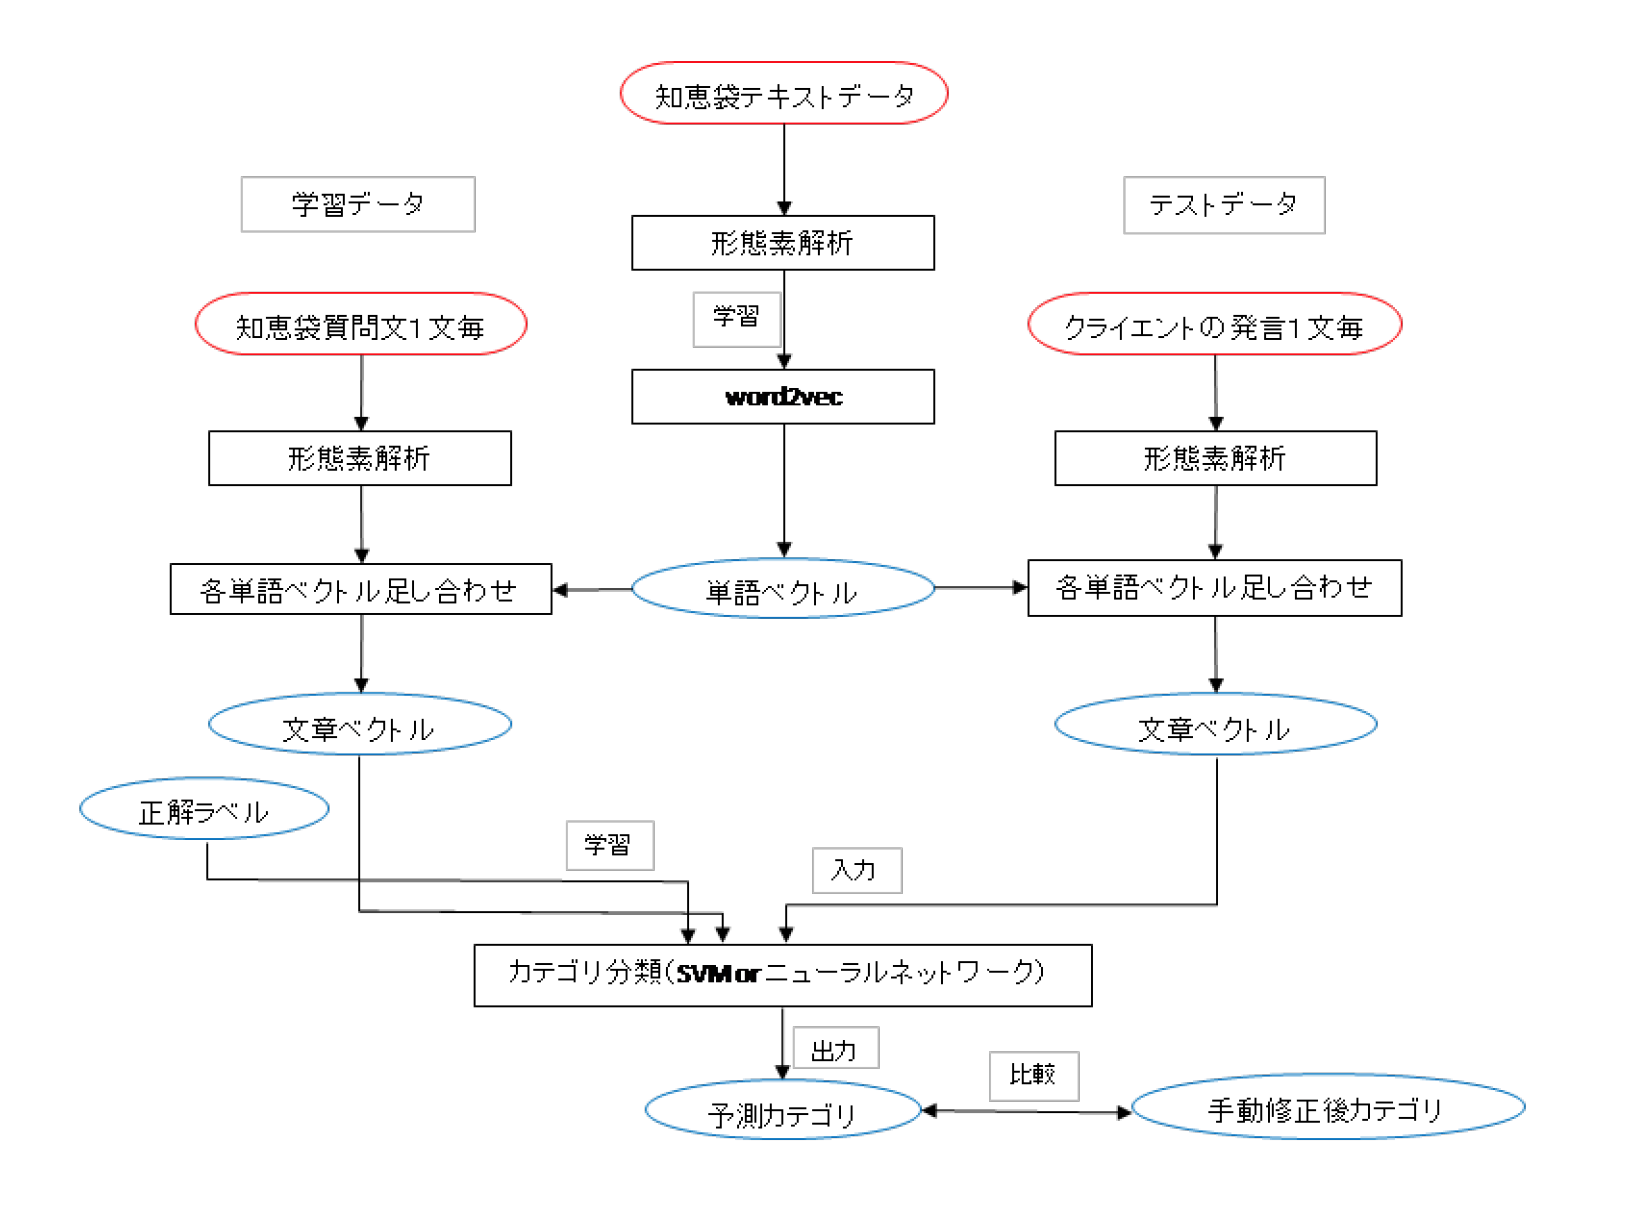
\includegraphics[width=\linewidth]{flowHayashida.png}
  \end{center}
  \caption{機械学習を用いたクライエント回答自動分類手法の流れ}
  \label{fig:flowHayashida}
\end{figure}

しかし林田らの分類手法では,クライエントの発言内容の中で,「不安です」のように,カウンセラーからの質問に対する返事などの短い文に対しては誤分類がなされているという問題が生じる.この問題解決を測るために,本研究では,クライエントの発言データにおいて,分類対象の文の前の文のword2vecベクトルを足し合わせて合計ベクトルを利用することを考え,林田の手法にこの改良を加えた.なお今回用いたカウンセリングの会話データには「スピリチュアル」に分類されるクライエントの発言がなかったので自動分類対象から除外している.また「自己」に関しては,コーパスであるYahoo!知恵袋に,「自己」に該当するカテゴリーがなかったため,自動分類対象から除外している.

\subsubsection{手法}
本改良手法では,γを0.01,0.001,0.0001,0.00001,Cを0.1, 1, 10, 100, 1000
の値で変えた計20通りの条件で,クライエントの発言内容を書き起こしたテキストデータのうち「愛」「交友」「仕事」いずれかのカテゴリーに分類されていた170文について,各文の前の文のword2vecのベクトルを足し合わせた合計ベクトルをSVMへの入力データとし,分類を行った.学習データは林田らの手法と統一し,機械学習手法も同様にソフトマージンSVMを用いた.%林田らの手法にて算出した各文のベクトルについて,その1つ前の文のベクトルを足し合わせたものを今回の手法における各文のベクトルとした.

\subsubsection{結果}
本改良手法の分類結果を表\ref{table:uetsuji1},\ref{table:uetsuji2}に示す.加えて,林田らの手法での分類結果を表\ref{table:hayashida3},\ref{table:hayashida4}に示す.今回の手法での30次元,γ=0.0001, C=100での正答率67.1%が,林田らの手法の最大正答率63.5%より高居結果が得られた.

\begin{table}
  \caption{前の文を考慮した時の40次元での分類結果(%)}
  \label{table:uetsuji1}
  \begin{center}
    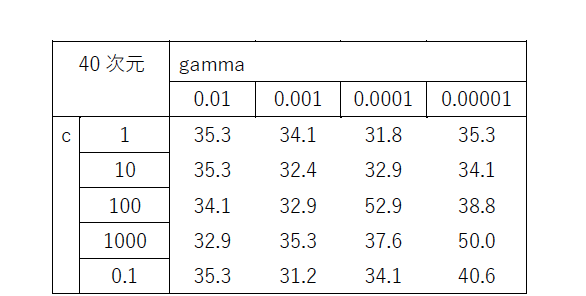
\includegraphics[width=\linewidth]{uetsuji1.png}
  \end{center}
\end{table}

\begin{table}
  \caption{前の文を考慮した時の30次元での分類結果(%)}
  \label{table:uetsuji2}
  \begin{center}
    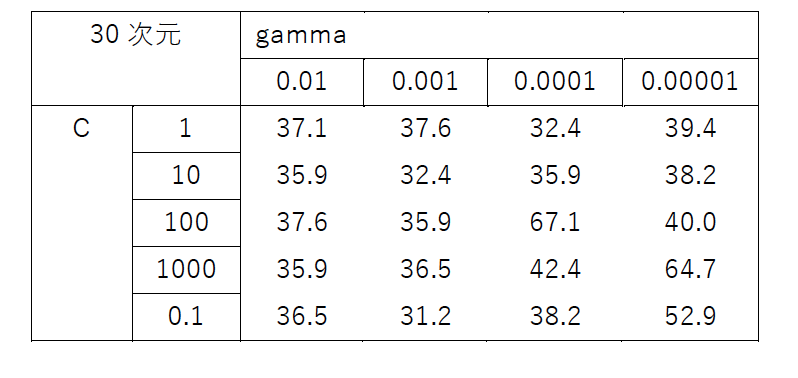
\includegraphics[width=\linewidth]{uetsuji2.png}
  \end{center}
\end{table}

\begin{table}
  \caption{前の文を考慮しない時の40次元での分類結果(%)}
  \label{table:hayashida3}
  \begin{center}
    
\includegraphics[width=\linewidth]{hayashida3.png}
  \end{center}
\end{table}

\begin{table}
  \caption{前の文を考慮しない時の30次元での分類結果(%)}
  \label{table:hayashida4}
  \begin{center}
    
\includegraphics[width=\linewidth]{hayashida4.png}
  \end{center}
\end{table}

% 今後の課題
SVMを用いた自動分類手法における今後の課題として,
\begin{itemize}
  \item 未分類グループが正解である文の場合の処理方法に関する検討
  \item 回答の1つ前の質問情報を加えることで,さらなる正答率の向上に関する検証
  \item 何文前まで遡ることで,正答率の向上につながるかに関する検証
\end{itemize}
などがあげられる.さらに,本提案システムへの自動分類手法の実装についても検討を行う必要があると考える.


\section{まとめ}

% 本節では,本章で提案した「会話の流れの視覚的分析システムシステム」に関する結論を説明する.本章では,カウンセラーの関心がクライエントが抱いている問題にどの程度傾聴しているかを,逐語録を読むよりよりわかりやすく理解させるために,「会話の流れの視覚的分析システムシステム」を提案した.

初心者のカウンセラーがどのような質問をし,それに対してクライエントからどのような回答が発せられているのかを可視化することで,クライエントが抱える問題に対して初心者のカウンセラーの関心がどの程度向いているかについて,どの程度理解が深まるかを検証するために,心理カウンセリングにおける会話の流れを可視化することで視覚的分析を行うシステムを提案し,実装を行った.


3.4.1項での可視化手法の比較評価から,積み重ね折れ線グラフに比べて,帯グラフの方が,「クライエントが抱いている問題に対してカウンセラーの関心がどの程度傾聴しているか」がよりわかりやすいという結果が得られた.さらに,3.4.2項での本提案システムの有用性の検証結果から,逐語録を読むだけの評価に比べて,本研究にて新たに提案した帯グラフを用いての評価の方が,「カウンセラーの関心がクライエントが抱いている問題にどの程度傾聴しているか」について,よりわかりやすいという知見を得た.

以上から,本研究で提案した帯グラフを用いた「会話の流れの視覚的分析システムシステム」は,1章で定義した心理カウンセリングの品質を向上する要素のうち,「カウンセラーの関心がクライエントが抱いている問題にどの程度傾聴しているか」之理解を支援する点において,既存手法よりも優れているということを実証した.




%%%%%%%%%%%%%%%%%%%%%%%%%%%%%%%%%%%%%%%%%%%%%%%%%%%%%%%%%%%%%  4章
%%認知の修正
\chapter{クライエントの認知の修正の視覚的分析システム}

%%%%%%%%%%%%%%%%%%%%%%%%%%%%%%%%%%%%%%%%%%%%%%%%%%%%%%%%%%%%%  4.1節
\section{はじめに}
心理カウンセリングにおいて,クライエントが心理カウンセリング中に「他人がクライエント自身に行った言動」ではなく,「クライエント自身が行った言動」の話の割合が多くなると,クライエントの認知の修正が進行しているといわれている.つまり,「相手の言動を変えることより,自分の言動を変えていくことに関心がある方が,認知の修正が進んでいる」\cite{zokad}とされる.さらに,クライエントの回答として「クライエントの身の回りの人の言動」に関する発言よりも「クライエント自身の言動」に関する発言が多くなると,クライエントの認知の修正が進行しているとされている.

しかし通常は,同じクライエントとカウンセラーで複数回の心理カウンセリングが行われるため,逐語録のテキストデータは膨大となり,全ての心理カウンセリングにおける逐語録を読むことでクライエントの認知の修正がどの程度進んでいるかを把握することは困難になる.この問題を解決するために,本章では「会話文中のどのタイミング会話文中の登場人物が誰に対しての,どの程度の言動を行ったか」を可視化することで,クライエントの認知の修正の理解を深めさせるシステムを提案する.


% クライエントは,多くの場合,より多くのクライエントの認知の修正は心理カウンセリングに進行し,「アクションの他人の話をクライエントに自分自身を行っている」.2「彼らが行っていることを言動について話す」の割合として言いる.言い換えれば,「あなた自身の言動を変えるのではなく,相手の言動を変えることに関心がある場合は,認知修正が進んでいる」[1].したがって,本研究では適切な心理カウンセリングの会話データから,「クライエントの言動」と「クライエントの言動を」分類し,結果を可視化することにより,クライエントの認知の修正の度合いを把握することができる,と考えた.

\section{認知の修正}%%%%%%%%%%%%%%%%%%%%%%%%%%%%%%4.2節

本研究で着目する心理カウンセリングはヨーガ療法にもとづいて行われている.ヨーガ療法における病理論は,約2800年前に記されたとされる「タイッティリーヤ・ウパニシャッド」に記されている,人間を五層に分けて考える「人間五臓説」にもとづいている\cite{kimura}.マンジュナート\cite{manjunath}は,変化する無常なるものを普遍的なものと錯覚する「理智の誤り」,すなわち「認知の誤り」(これ以降,本論文では「認知」と統一して記す)を基準として,病気について
\begin{itemize}
  \item 「認知の誤り」から生じない感染症や外傷などの病気
  \item 「認知の誤り」から生じる心身病などの病気
\end{itemize}
の2種類に分類される.特に後者は現代心身医学のストレス認知的評価説% (Lazarus, Folkman 1984)
\cite{Lazarus}とほぼ一致してるといえる\cite{Darshana}.


鎌田\cite{kamata2002}によると, カウンセラーの重要な役割は,クライエントが不当に他人に介入することなく,他者との協力関係を形成することが可能であるようにクライエントを奨励することである.そのため,不当に他人の言動や感情に介入することなく,クライエント自身の言動や感情を見つけることが重要である.

1980年代に現代のアドラー心理学を日本に初めて取り入れた野田\cite{zokad}は,神経症者の基本的な心理的構えを「悪いあの人」「かわいそうな私」と表現している.神経症者はこの「悪いあの人」「かわいそうな私」といった文句・批判・愚痴を含んだ言動を形成し,社会から離れていこうとする.これを,責任転嫁を目的とした自己欺瞞(self-deception)と呼ぶ\cite{Darshana}.しかし「悪いあの人」と言うことでクライエントは相手に自分の心を支配される.「つまり,相手の言動次で自分の心の安定が左右される」.これを「状況依存(context-dependent)」と呼ばれている.
% \begin{itemize}
%   \item 「自己努力」(感謝・貢献)「私がBさんにこうしてあげた」認知の修正が進んでいる
%   \item 「状況依存(context-dependent)」(「悪いあの人」「かわいそうな私」文句・批判・愚痴)「私がBさんに思い通りになってほしいと思う」認知の修正が進んでいない
% \end{itemize}

この状態が続くと相手が変わらない限りは自分が幸せではないという思考の元で過ごすことになり,「自己努力」での改善を放棄してしまうとされる\cite{zokad}.ヨーガ療法では,認知の修正の進行に伴い,クライエントがこのような「状況依存」から抜け出し,「自己努力」で自身の心の安定を作成することができるように援助することを目標としている.つまり,「今ここで私にできること」として感謝・貢献をクライエントが自身で模索し実践できるように,カウンセラーがクライエントを常に勇気づけ(encouraging)することが目標である.この方向と一致する心理学として,「全ては個人が選択決断している」という実存主義(existentialism)的立場をとるアドラー心理学が挙げられる.


\section{システム要件}
%一連の文章の中から,場面ごとに登場人物が誰に言動を起こしたか把握したい,会話文や物語の人間関係を想起する必要がある場面がある.たとえば
心理カウンセリングにおいて,クライエントは「相手の言動を変えることより,自分の言動を変えていくことに関心がある方が,認知の修正が進んでいる」\cite{zokad}とされている.また,クライエントの回答として「クライエントの身の回りの人の言動」に関する発言よりも「クライエント自身の言動」に関する回答が発せられた方が,クライエントの認知の修正が進行しているとされている.

図\ref{fig:arrow}に,鎌田\cite{鎌田穣2002臨床}が提唱した,クライエントの認知の修正の判断のための矢印技法による,「認知の修正が進んでいる時に現れる矢印」と「認知の修正が進んでいない時に現れる矢印」を示す.図\ref{fig:arrow}の各番号の丸や矢印に対する意味を下記に記す.(1),(2)は「自己努力」,(3),(4),(5)は「状況依存」に分類される.

\begin{figure}
  \begin{center}
    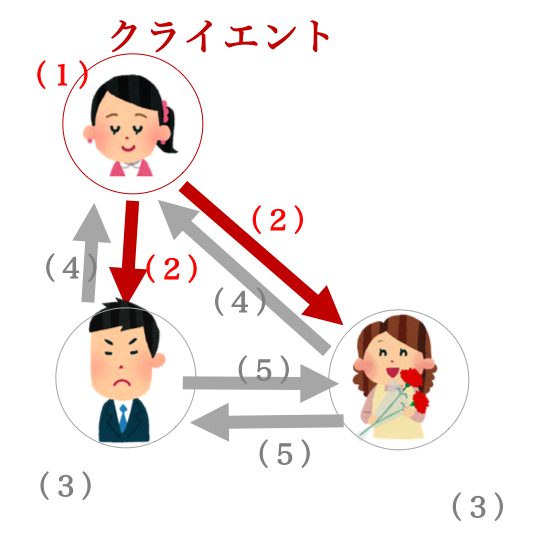
\includegraphics[width=\linewidth]{arrow.png}
  \end{center}
  \caption{認知の修正が進んでいる時に現れる矢印と進んでいない時に現れる矢印}
  \label{fig:arrow}
\end{figure}

\begin{enumerate}
  % \renewcommand{\labelenumii}{(\arabic{enumii})}
  \renewcommand{\labelenumi}{(\arabic{enumi})}
  \item 「クライエント自身」の内的感情・「クライエントの周囲の人」に向けられていない「クラ
    イエント」一人の行動
    \item 「クライエント自身」から「クライエントの周囲の人」へのポジティブな行動
    \item 「周囲の人」の内的な陰性感情の予測や,他者に向けられていないその
      「周囲の人」一人のネガティブな行動
    \item 「クライエントの周囲の人」から「クライエント自身」へのネガティブな行動
    \item 「クライエントの周囲の人」から「クライエントの周囲の人」へのネガティブな行動
\end{enumerate}



以上から,「クライエントの身の回りの人の言動」か「クライエント自身の言動」かを,会話データを基に有向グラフの人間関係図で可視化することで,クライエントの認知の修正の具合に関して,直感的に理解できるのではないかと考える.

Vanら\cite{van2009mapping}がユーザーによって指定された``B of A''および``A and B''の関係を有向グラフで表現した視覚的分析システムの研究が行われている.しかし,この可視化手法は接続詞や前置詞ベースで単語をつなげており,本研究で必要とされる登場人物が誰に対して言動したかを視覚的に把握することは難しい.田中ら\cite{tanaka}は効率的に話の内容を想起できるように,登場人物を共起関係で結び,頻出の登場人物や共起を強調させて表すインタフェースを実装した.しかし,この可視化手法は登場人物同士を共起関係の線のみで結んだ無向グラフとして可視化しているのみで,ある場面において,登場人物がが誰に対して言動したかをそのグラフから把握することはできない.また,この可視化手法では話の章毎のみの可視化となっており,会話文内のどのシーンからクライエントの認知の修正が進行したかを把握することは困難と考える.

本研究では,カウンセリングの会話内に登場する人々の間でどのような言動が誰に対して発せられたかを人間関係図を用いて可視化を行うことで,クライエントの認知の修正について視覚的分析を行うシステムを提案し,実装を行う.本提案システムでは時系列に沿って,カウンセリングの各会話文内容から主語と目的語を含んだ言動の情報を可視化することを試みる.

% 本研究の「クライエントの認知の修正の視覚的分析システム」では,心理カウンセリングの会話文中に登場する人物たちについて,「会話内のどの時間に登場人物が誰に対してどの程度言動を発したか」を可視化することで,クライエントの認知の修正に対するカウンセラーの理解を深めることを目的とする.そこで,時系列に沿って,会話内容から主語と目的語を含んだ言動の情報を可視化することにより,上記の可視化が可能であると考えた.

% 以上のように,どのような場面で登場人物が誰に言動したかを文書から抽出することが求められている.それに対し本研究では,登場人物が誰にどのような言動をとったかを時系列で可視化することで,上記のニーズを満足できるのではないかと考えた.このような要求に対し,本研究では登場人物が誰に言動したかという人間関係図を時系列にそった可視化を試みた.





% \subsubsection{クライエントの分析}%%%%%%%%%%%%%%%%%%%%%%%%%%%%%
%
%
%
% % 心理カウンセリングで,「自分の言動を変えるのではなく,相手の言動を変えることに関心がある人は,認知を修正するに進んでいる」と言われている.ときに,クライエントの答え「クライエント自身の言動」ではなく答えるクライエントの認識の修正が進んでいると言われて, 『クライエントの周りの人々の言動を.』
%
% 本研究では,「登場人物が誰にどの程度言動を行っているか」を可視化することにより,クライエントの認知の修正の状態の理解を深める.そこで,時系列に沿って,会話内容から主語と目的語を含んだ言動の情報を可視化することにより,上記の可視化が可能であると考えた.




% クライエントの認知補正の分析は,何らかの形でのように説明したクライエントの言動のカテゴリーを使用 図.2 動作は,クライエントの周りの人々が行っていたものが挙げられる. 鎌田\cite{kamata2002}によると,カウンセラーの言動や感情を重要な役割は,クライエントが自己決意と自己責任を取ると不当に他人に介入することなく,他者との協力関係を形成することができるようにクライエントを奨励することである.だから,不当に他人の言動や感情に介入することなく,クライエント自身の言動や感情を見つけることが重要である.
%
%   心理カウンセリングで,「自分の言動を変えるのではなく,相手の言動を変えることに関心がある人は,認知を修正するに進んでいる」と言われている.ときに,クライエントの答え「クライエント自身の言動」ではなく答えるクライエントの認識の修正が進んでいると言われて, 『クライエントの周りの人々の言動を.』

%\subsection{要件抽出}

図\ref{fig:arrow}のような人間関係図を,心理カウンセリングの会話文中の各タイミングから抽出して可視化するには,「会話文中のどのタイミングで登場人物が誰に対してどの程度の言動を行ったか」の情報が必要である.「ある登場人物が別の登場人物に対して行った言動」は,
\begin{itemize}
  \item 言動を表す動詞
  \item その動詞の主語
  \item その動詞の目的語
\end{itemize}
の3つの情報から成り立っており,これらの情報を心理カウンセリングの会話文から得るために,各会話文に対して,係り受け解析を行い,登場人物と動詞の係る―係られる関係を取得する.

% Vanら\cite{van2009mapping}がユーザーによって指定された``B of A''および``A and B''の関係を有向グラフで表現した視覚的分析システムの研究が行われている.しかし,この可視化手法は接続詞や前置詞ベースで単語をつなげており,本研究で必要とされる登場人物が誰に対して言動したかを視覚的に把握することは難しい.
%
% 田中ら\cite{tanaka}は効率的に話の内容を想起できるように,登場人物を共起関係で結び,頻出の登場人物や共起を強調させて表すインターフェースを実装した.しかし,この可視化手法は登場人物同士を共起関係の線のみで結んだ無向グラフとして可視化しており,その場面は登場人物がが誰に対して言動したかをそのグラフから把握することはできない.また,この可視化手法では章ごとのみの可視化となっており, 彼らの可視化を用いても,会話文内のどのシーンからクライエントの認知の修正が進行したかを把握することは困難である.

本システムにおける可視化の表現手法として,カウンセリングの会話内の登場人物が行った言動のうち,目的語をもたないものを円で,「別の登場人物」を目的語とするものを矢印で表現することにした.同一の主語・目的語の組み合わせをもつ言動がある場合には,円の大きさ・矢印の太さを大きくすることで,「ある登場人物が別の登場人物に対して行う言動」がどの程度行われているかは,各図形の大きさや太さで表現されるものとする.その言動が「会話文中のどのタイミングで」行われているかを可視化するためにスライドバーを用いる.
% 以上を踏まえて,本提案システムでは次項に説明する前処理の実装を行った.



% 本研究における「クライエントの認知の修正の視覚的分析システム」では,「クライエント自身の言動」または「クライエントの周りの人の言動」について,「会話文中のどのタイミングで登場人物が誰に対して,どの程度の言動を行ったか」を可視化することにより,クライエントの認知の修正の評価を支援することを目的とする.本研究では時系列順に会話内容をテキストで言動の主語と目的語を可視化することにより,上記のニーズを満たすことができると考えた.




\section{システム実装} %%%%%% 4.3

\subsection{前処理部} %%%%%%%% 4.3.1


図\ref{fig:charaFlow}に,クライエントの認知の修正の視覚的分析システムの流れを示す.本節では,会話文中のどのタイミングで登場人物が誰に対して,どの程度の言動を行ったかを可視化する人間関係図を生成するための前処理として,登場人物データと言動データを抽出する手法を説明する.%テキストデータ内のオブジェクトデータ.

まず,心理カウンセリングの逐語録のテキストデータに対して,形態素解析と係り受け解析を施した結果が,本提案システムへの入力データとなる.この入力データから,心理カウンセリングの会話内に登場する人物と,言動を表す動詞を抽出する.次に,各動詞の主語と目的語となる登場人物をその動詞と対応付けて,同じ主語―目的語のペアである動詞の個数をカウントする.このカウント数が,人間関係図のグラフ可視化における円の大きさや矢印の太さとして反映される.以降,本提案システムの前処理の流れの各段階について説明する.


\begin{figure}
  \begin{center}
    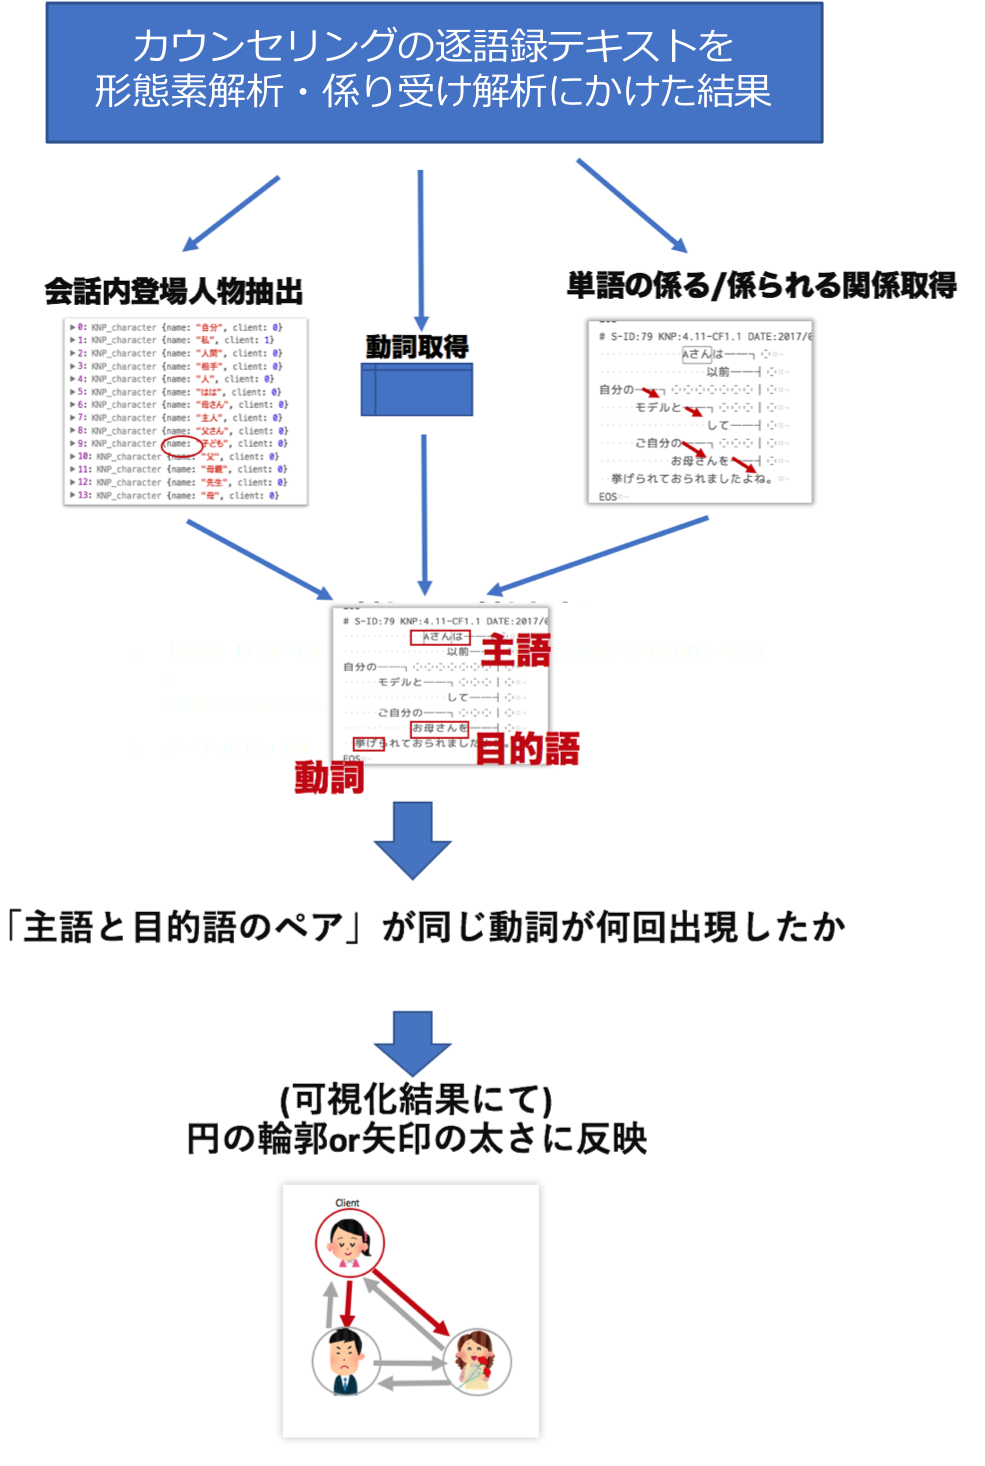
\includegraphics[clip,width=13.0cm]{charaFlow.png}
  \end{center}
  \caption{認知の修正の視覚的分析システムの流れ}
  \label{fig:charaFlow}
\end{figure}





\subsubsection{(1)係り受け解析}


係り受け解析,または構文解析(syntactic analysis あるいは parse)とは,文章に形態素解析を施して単語ごとに切分けた後に,その間の関連(修飾-被修飾など)といった,統語論的(構文論的)な関係を図式化するなどして解析する手続きである.構文解析を行う機構を係り受け解析器(parser)と呼ぶ.本提案システムでは入力データに対して,形態素解析後の係り受け解析や,後述する格の判断にKNP(係り受け解析器)\cite{KNP}を用いるため,逐語録テキストに対して,日本語形態素解析器のJUMAN\cite{juman}で形態素解析を行うことで,そのままKNPで係り受け解析ができる流れにした.



\subsubsection{(2)登場人物と動詞の抽出}


% 本項では,文章中の登場人物を抽出する手法について説明する.元の文は,係り受け解析前にまず日本語形態素解析器JUMAN\cite{juman}によって形態素解析されている.
 JUMANは,形態素解析時に,独自の辞書によって,日本の各単語を品詞やカテゴリーに分類する.JUMANにより「人」のカテゴリーに分類された単語を抽出することにより,文章中の登場人物の抽出を行う.%心理カウンセリングの会話書き起こしテキストデータをKNPに入力されたときに,このシステムの入力は,KNP \cite{KNP}(係り受け解析器)の出力結果である.

また,JUMANの品詞解析機能を用いて,心理カウンセリングの会話テキスト全文章から,登場人物と同様に「品詞:動詞」となっているものをリストアップした.さらに,それぞれの動詞とそれに係る登場人物名詞との係り受け関係を把握するよう保存した.


% \subsubsection{動詞の主語と目的語の抽出}

\subsubsection{(3)動詞の主語の抽出}


各「動詞」に係る文節に含まれる「登場人物」の名詞のうち,
\begin{itemize}
  \item KNPにおいて,「私が」「Bさんが」等,<ガ格>として出力されたもの
\end{itemize}
に含まれるものを,その動詞に対する主語とした.

「私は」「Bさんは」等<ハ格>と思われるものに対してKNPには格の分類が存在せず,またこれらの文節に含まれる登場人物は,「Aさんは先生にこれをあげたい」の「Aさん」のように主語になるものと,「BさんはAさんがこれをあげた人だ」の「Bさん」のように目的語になるものがあるため,今回は<ハ格>を無視した.

\subsubsection{(4)動詞の目的語の抽出}


各「動詞」に係る文節に含まれる「登場人物」の名詞のうち,

\begin{itemize}

  \item KNPにおいて,「私を」「Bさんを」等,<ヲ格>として出力されたもの
  \item KNPにおいて,「私に」「Bさんに」等,<ニ格>として出力されたもの
\end{itemize}
に含まれるものを,その動詞に対する目的語とした.

\subsubsection{(5)各登場人物の誰に対する言動の数のカウント}

その後,心理カウンセリングの会話テキスト内で,同じペアの主語と目的語を持っている動詞の数をカウントした.このカウントから,「会話文中のどのタイミングで登場人物が誰に対して,どの程度の言動を行ったか」がわかり,円や矢印が意味する動詞の数は,後述する会話データの可視化処理部の人間関係図のグラフにおいて,円の大きさや矢印のストローク幅に反映されている.

%%%%%$ 認知の修正可視化結果

\subsection{会話データの可視化処理部}

本項では,本提案システムの可視化部分について説明する.図\ref{fig:dummyChara}に模擬会話データを用いた本システムの可視化結果例を示す.可視化結果は,「人間関係図」「スライドバー」「原文表示ビュー」3つの項目から構成されている.可視化処理の実装に,D3.js\cite{vand3}を使用した.以下に各項目について説明する.%それが書かれた書き起こし産物に基づきる.

\begin{figure}
  \begin{center}
    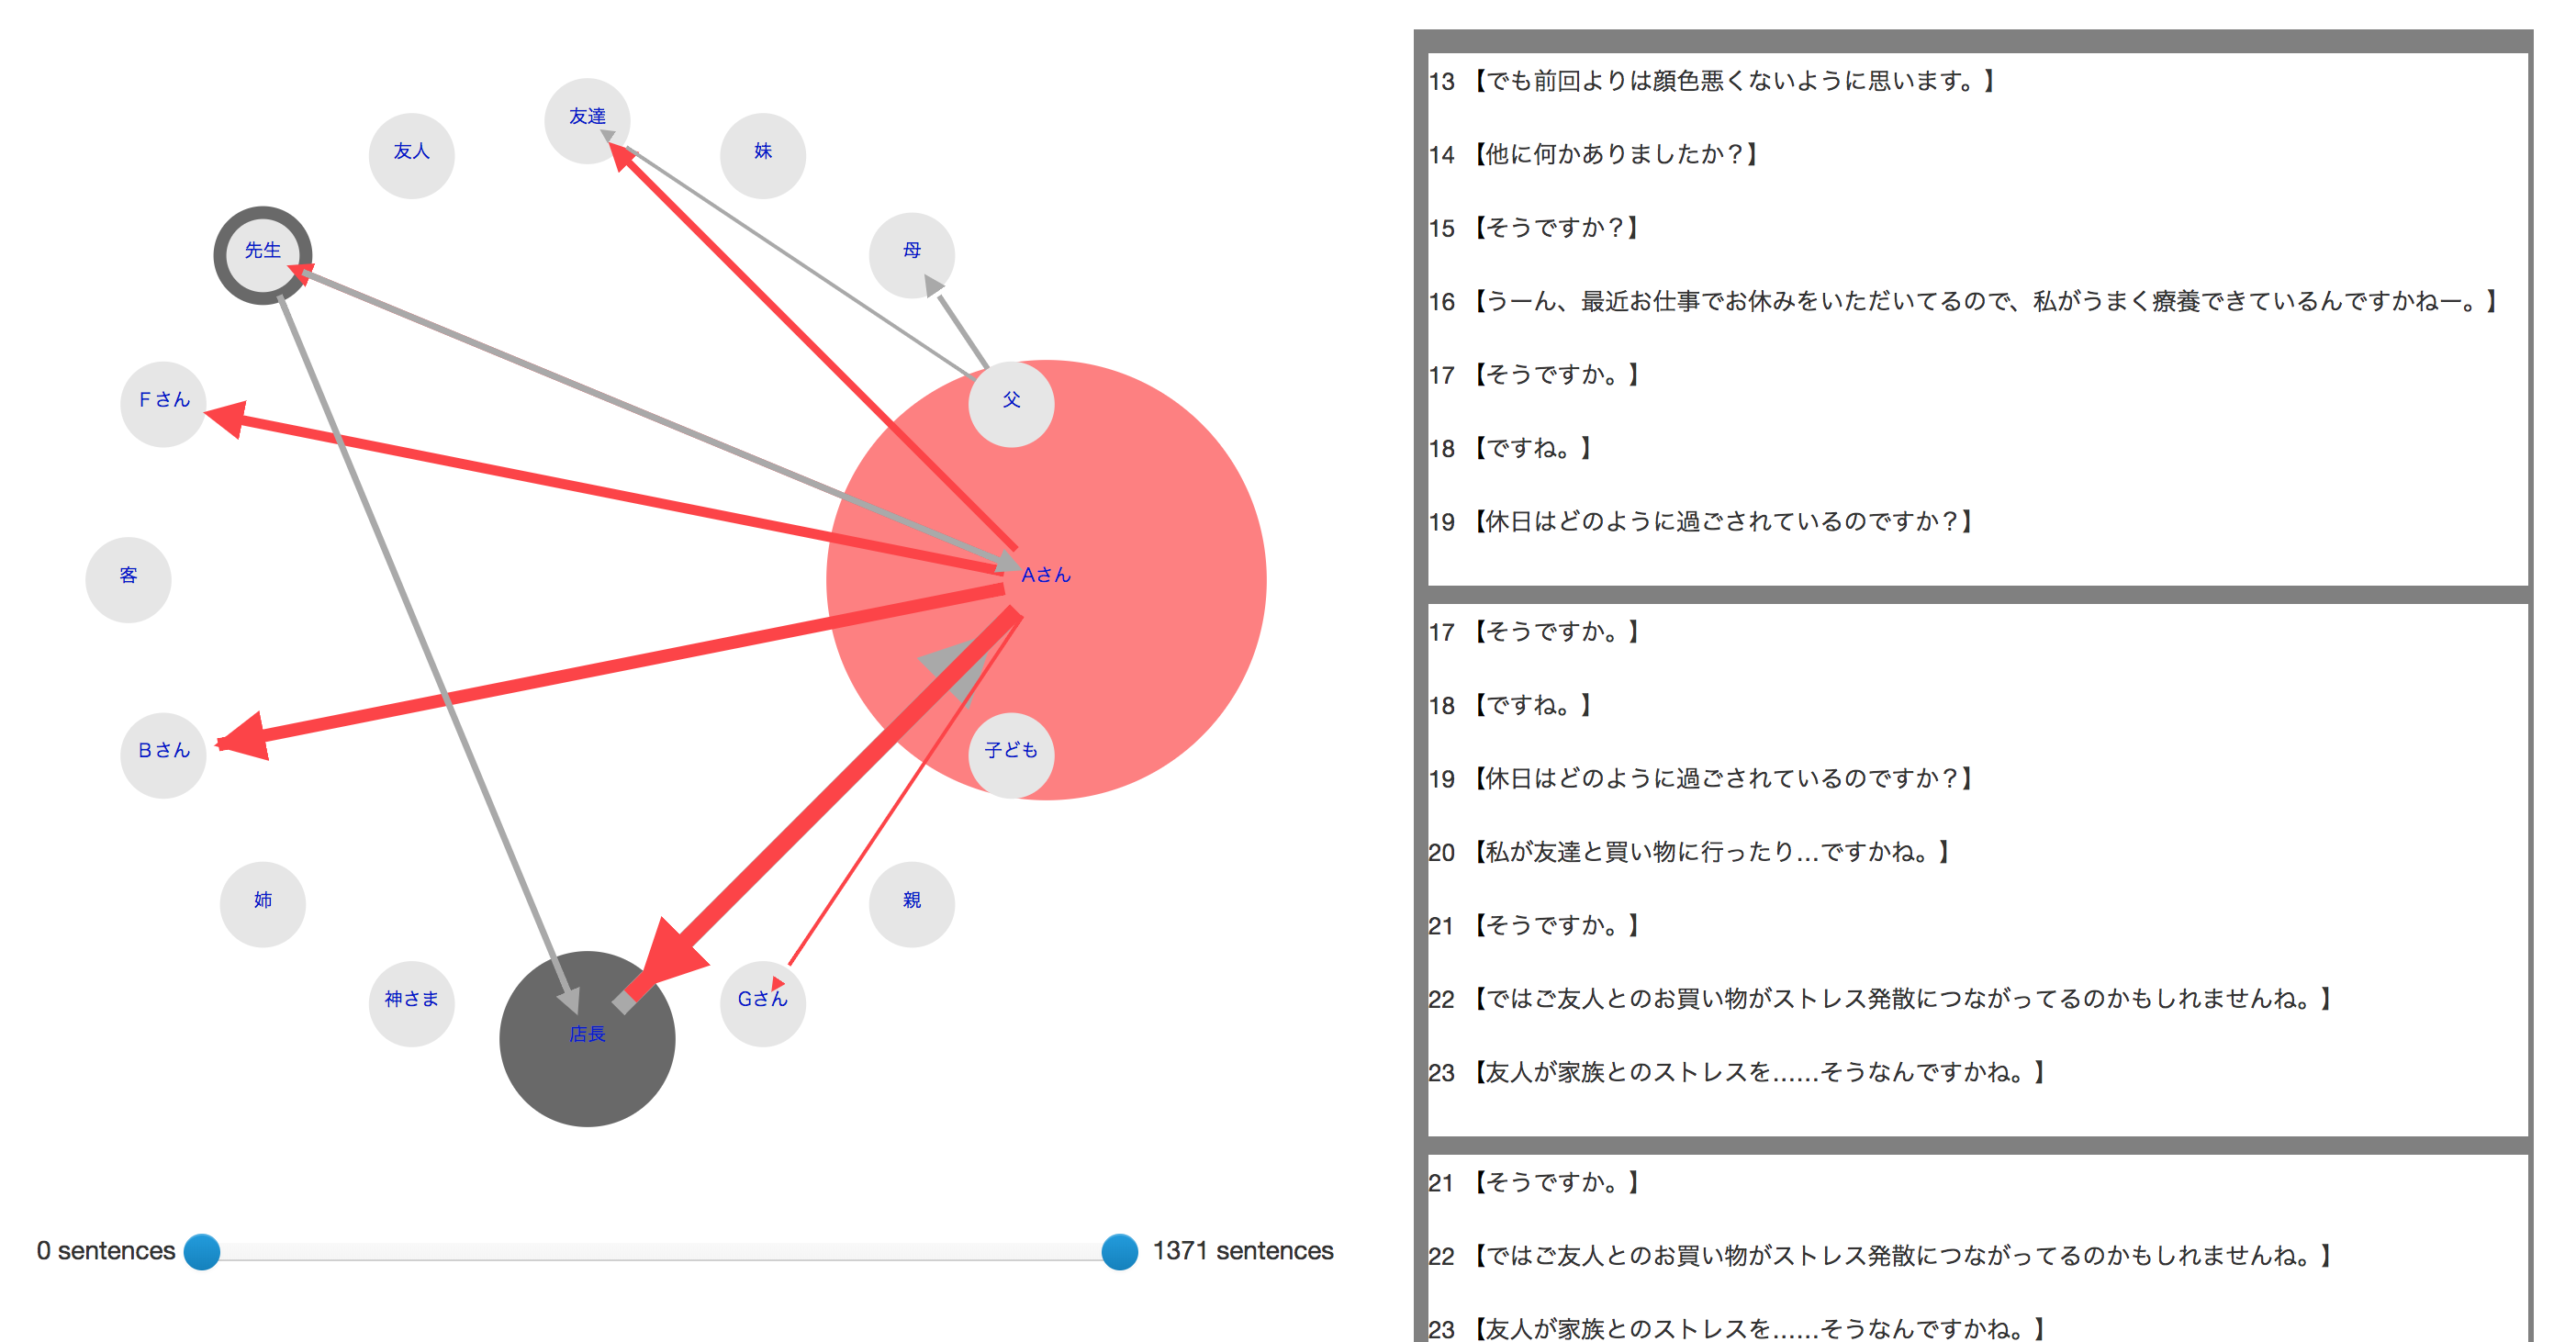
\includegraphics[width=\linewidth]{dummyChara.png}
  \end{center}
  \caption{「クライエントの認知の修正の視覚的分析システム」の可視化結果(模擬会話データ)}
  \label{fig:dummyChara}
\end{figure}

\subsubsection{(1)有向グラフの人間関係図}

% Vanら\cite{van2009mapping}は文章を分析し,``B of A''および``A and B''の関係を有向グラフで表現した.しかし
本研究では,「会話文中のどのタイミングで登場人物が誰に対して,どの程度の言動を行ったか」を有向グラフで可視化した.さらに,有向グラフに色分けを用いて,心理カウンセリングの会話テキスト内の人間関係図を可視化することで,クライエントの認知の修正に関する分析を試みる.

%\subsubsection{}

次に,会話文中の登場人物の内的感情や一人で完結した言動を表す円形について説明する.
心理カウンセリングの会話文内に登場する人物が円周上に一覧として並べられ,「その会話中でその人物が起こし,目的語を持たない言動」の数は,円の大きさで表されている.クライエント自身であれば円はピンク,それ以外は水色で表している.鎌田\cite{鎌田穣2002臨床}が提唱した図\ref{fig:arrow}に示す矢印技法において,
\begin{itemize}
  \item ピンクの丸……「クライエント自身」の内的感情・「クライエントの周囲の人」に向けられていない「クライエント」一人の行動
  \item 水色の丸……「周囲の人」の内的な陰性感情の予測や,他者に向けられていないその
  「周囲の人」一人のネガティブな行動
\end{itemize}
を表している.したがって,ピンクの丸がより大きくなっていく仮定を確認できれば,認知の修正が進行していると判断できると考える.

%\subsubsection{}
会話文中の登場人物が別の登場人物に対して行った言動を表す矢印は,登場人物から別の登場人物への言動の発生を表している.さらに,前処理部でカウントした,主語・目的語の組み合わせが同じ動詞を1つの矢印にまとめ,その動詞の数をその言動の数とみなし,矢印の太さで表現している.


\begin{itemize}
  \item 「クライエント自身」から「クライエントの周囲の人」へのポジティブな言動:(「ネガティブだが,もしもの話」の場合を含む)→赤の矢印
  \item 「クライエント自身」から「クライエントの周囲の人」へのネガティブな言動:(「ポジティブだが,もしもの話」の場合を含む)→青の矢印
  \item 「クライエントの周囲の人」から誰かへのポジティブな言動:(「ネガティブだが,もしもの話」の場合を含む)→オレンジの矢印
  \item 「クライエントの周囲の人」から誰かへのネガティブな言動:(「ポジティブだが,もしもの話」の場合を含む)→緑の矢印
\end{itemize}

したがって,赤やオレンジの矢印が多くなったり太くなったりするほど,認知の修正が進行していると判断する.

\subsubsection{(2)スライドバー}

本システムでは,心理カウンセリングの会話の全文データのうち,200文分を抽出して人間関係図に可視化表示している.初期表示では0文目〜200文目を可視化表示している.スライドバー上の青丸にマウスカーソルを合わせると,いま何文目から何文目までのデータについて可視化表示を行っているかを吹き出しで表示する.
さらに,青丸を動かすことで,可視化表示する会話文データの範囲を変更することができる.


\subsubsection{(3)原文表示機能}

人間関係図上に表示されている登場人物の円をクリックすると,「その登場人物が登場する心理カウンセリングの原文箇所」が,画面右側に表示される.
矢印をクリックすると,右側に「その矢印に該当する言動を示す心理カウンセリングの原文箇所」が,画面右側に表示される.
原文表示で下線が引かれている場所に,そのクリックした矢印に該当する動詞が含まれている.


\section{システム評価と考察} %%%%%%%%%%%%%%%%%%%%%%%%% 4.4

本節では,本提案システムの有用性之評価として,本提案システムを用いることでクライエントの認知の修正に関する視覚的分析にどのように支援できるかについて検証を行う.


% \subsection{熟練カウンセラーによる} %%%%%%%%%%%%%%%%%%%%%%% 4.4.1

% 本項では,
実際の心理カウンセリングの会話データを,本提案システムにて可視化表示を行い,熟練カウンセラーの方によるシステムの試用評価を行った.%この結果に対するシステム評価および考察については次項で説明する.

本評価では,同じカウンセラーとクライエントで行われた5回分の実際の心理カウンセリングのテキストデータを時系列順に並べ,1つのテキストデータとした.このテキストデータをJUMANで形態素解析し,KNPで係り受け解析した後,その係り受け解析結果を本システムに入力し,会話データの可視化表示を行った.本システムによる可視化結果を図\ref{fig:caseFirst},\ref{fig:caseSecond},\ref{fig:caseThird}に示す.

図\ref{fig:caseFirst}(最初2回のカウンセリング)に対する可視化結果より,クライエントである「Aさん」自身が行った「Bさん」と「Fさん」に対するネガティブな言動が目立っていることがわかる.さらに,図\ref{fig:caseSecond}(3,4回目のカウンセリング)の結果より,新たな登場人物として「店長」からクライエント自身へのネガティブな言動に関して,クライエントが言及するようになったことがわかった.しかし,図\ref{fig:caseThird}(5回目のカウンセリング)では,クライエント自身から「店長」へのポジティブな言動が目立つようになったことが,可視化結果より把握できていることがいえる.


\begin{figure}
  \begin{center}
    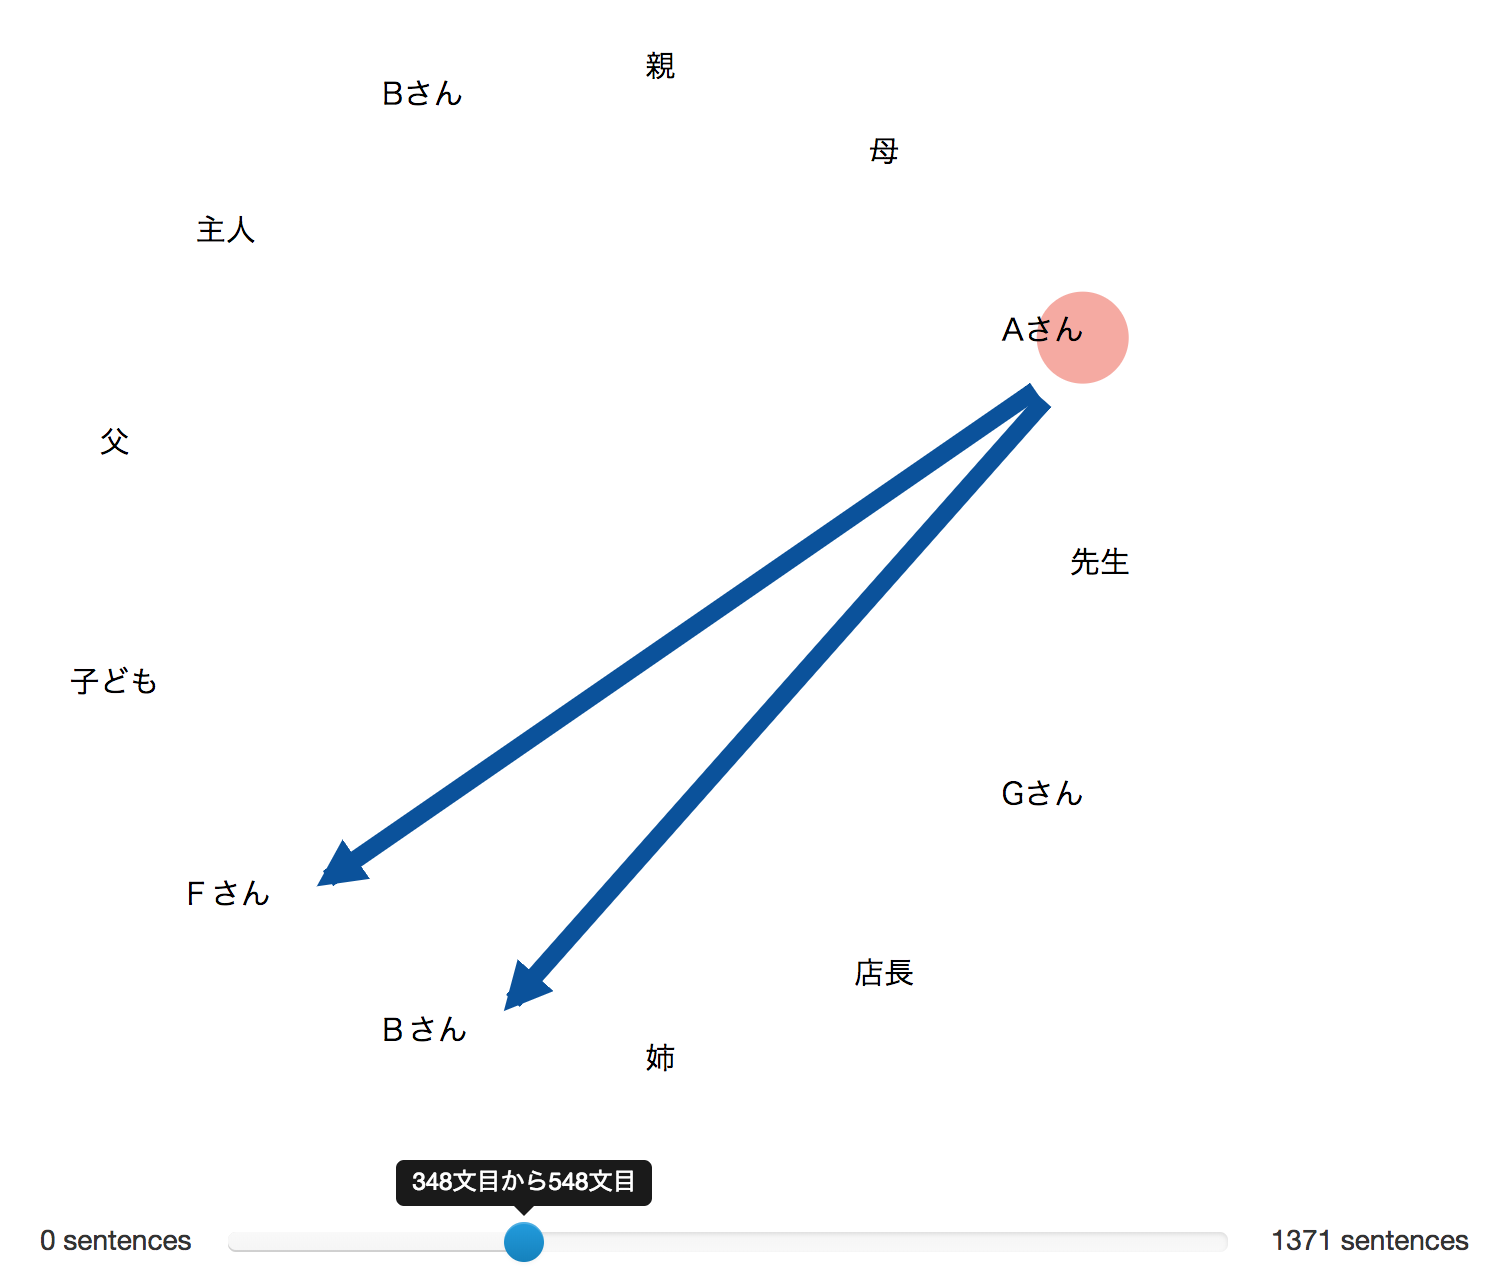
\includegraphics[width=\linewidth]{caseFirst.png}
  \end{center}
  \caption{カウンセリング5回分の中の348文目から548文目における可視化結果}
  \label{fig:caseFirst}
\end{figure}

\begin{figure}
  \begin{center}
    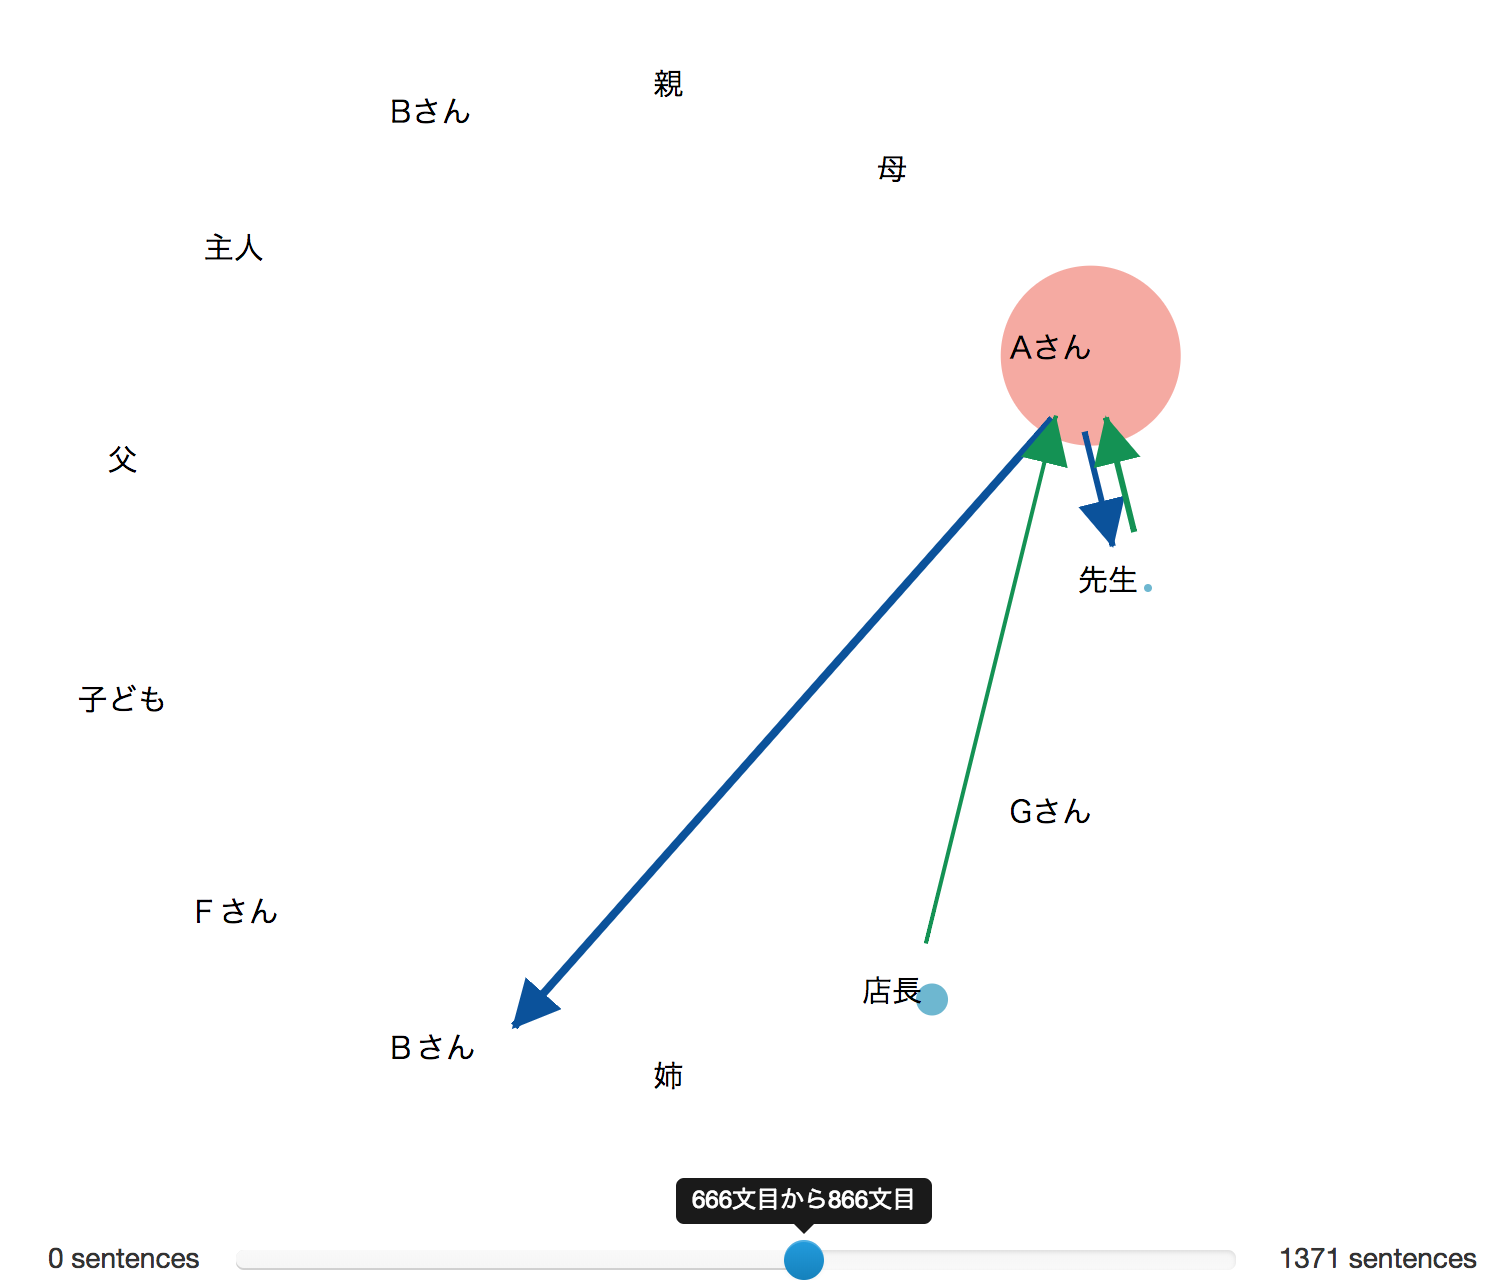
\includegraphics[width=\linewidth]{caseSecond.png}
  \end{center}
  \caption{カウンセリング5回分の中の666文目から866文目における可視化結果}
  \label{fig:caseSecond}
\end{figure}

\begin{figure}
  \begin{center}
    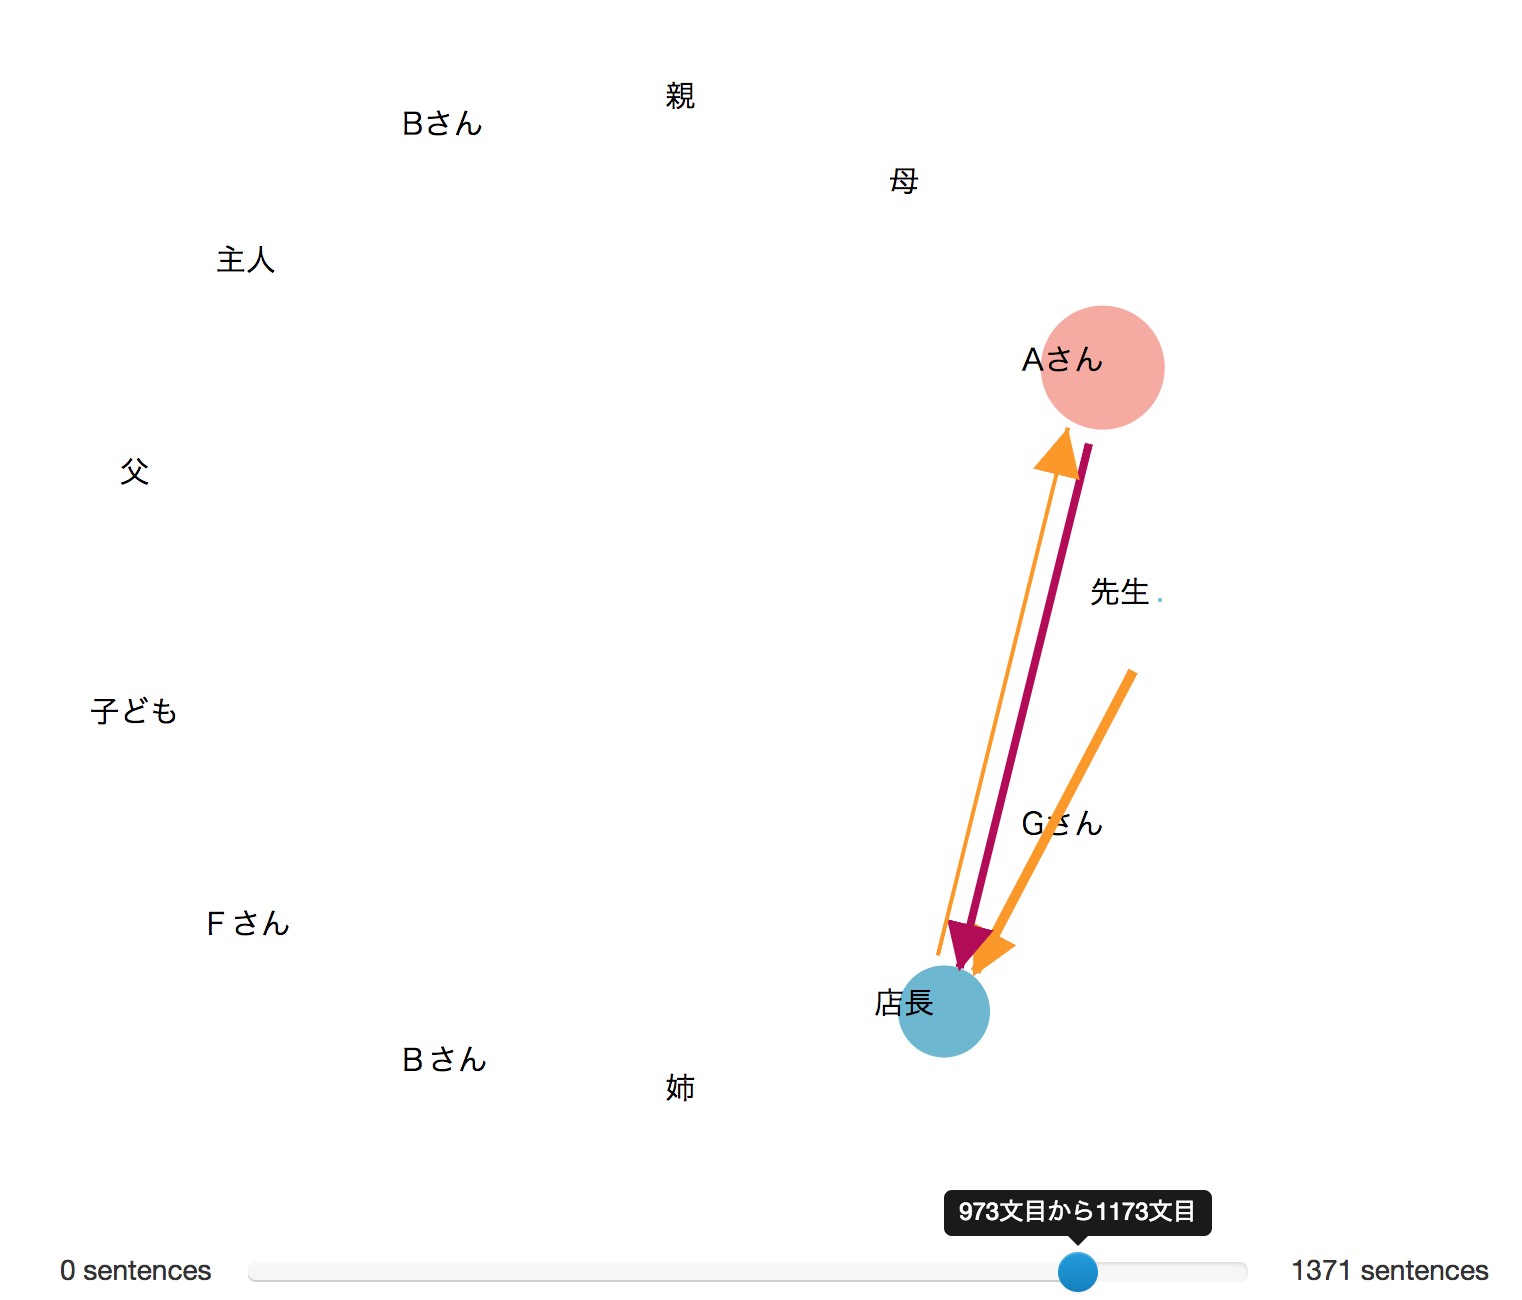
\includegraphics[width=\linewidth]{caseThird.png}
  \end{center}
  \caption{カウンセリング5回分の中の973文目から1173文目における可視化結果}
  \label{fig:caseThird}
\end{figure}

% The expert counselor said that he found out that the idea ``I want B to follow my will'' disappeared
and self-closed task increased. Progress of correction of cognition could be confirmed by changing the quantity of arrows (Overall view of multiple counseling) and confirming the quality in original text display. We consider that our proposed character chart visualization helps counselors find out that some kind of client's cognitive fixes were made.
%
% 図1心理カウンセリング1
% 図2心理カウンセリング2

% \subsection{熟練カウンセラーからのコメントと考察} %%%%%%%%%%%%%%%%% 4.4.2

次に,このカウンセリングの会話データについて,矢印の色分けをなくしたものと色分けを施したものの2パターンの可視化結果について,熟練カウンセラー1名に見ていただくことで本システムの試用評価を行い,以下に示す評価結果が得られた.
\begin{enumerate}

  \item 「私がBさんを思い通りにしたい」というような
  自分で閉じた話題「セルフタスク」への変化がみてとれた.
  \item クライエントから店長に向かっている矢印が増えた.
  \item 複数の心理カウンセリングの全体俯瞰をすることで,矢印の量の変化が確認できた.
  \item 原文表示での質の確認により,認知の修正の進行が確認できた.
\end{enumerate}

さらに,熟練カウンセラーからのコメントとして,カウンセリングの中盤になって「クライエント自身」の内的感情・「クライエントの周囲の人」に向けられていない「クライエント」一人の行動,すなわちセルフタスクが増えたことで,認知の修正の評価を支援できたと考えられる.
また,「色付きの方がネガティブとポジティブについてわかりやすい」というコメントを得た.


「
赤とオレンジの増加が最後は認められ,このあたりから認知の修正の可能性が
認められるようになったと考えます.クライエントほんにんの内的感情状態がネガティブなのかポジティブなのかが
わかるようになると大変役立つと思いました.大きさだけでは,ネガティブかど
うかがわからないところです.
」といったコメントが得られた.ポジティブかネガティブかを可視化することで,単なる矢印よりもさらにわかりやすく「クライエントの認知の修正の進行」の評価を支援できることが示唆される.

そして,「感謝・貢献」と「悪いアイツかわいそうな私」を言語処理で分別するのは厳しい
といったコメントを得た.矢印の分類の信憑性の問題は,テキスト分析の問題なので,今後の課題であると考える.


\section{まとめ}%%%4.5節
本節では,「クライエントの認知の修正の視覚的分析システム」についてのまとめを説明する.本章では,「会話文中のどのタイミングで登場人物が誰に対して,どの程度の言動を行ったか」を有向グラフで可視化することで,クライエントの認知の修正の分析を支援できることを提案した.

前項の熟練カウンセラーからのコメントから,「会話文中のどのタイミングで登場人物が誰に対して,どの程度の言動を行ったか」を有向グラフで可視化することで,今日の事例検討会の通り逐語録を読むことに比べて,クライエントの認知の修正の分析を支援できることが示唆される.
本研究では無向グラフなどの他の可視化手法との比較実験までには至らなかったが,今後は比較実験を行うことで上記の示唆についてより確かな知見が得られるのではないかと考える.


\chapter{結論}%%% 5章

本章では,本研究における結論,および,今後の課題について述べる.

\section{本研究における結論}



本研究ではまず,1章で定義した心理カウンセリングの品質向上のために重要な要素の一つに考えた「クライエントが抱える問題に対してカウンセラーの関心がどの程度傾聴しているか」の理解を支援するために,3章にて提案した帯グラフを用いた「会話の流れの視覚的分析システムシステム」が,逐語録を読むだけの評価や積み重ね折れ線グラフを用いた評価よりも優れているという検証結果が得られた.具体的には,3.4.1項での可視化手法の比較実験結果から,積み重ね折れ線グラフに比べて,帯グラフの方が,「クライエントが抱いている問題に対してカウンセラーの関心がどの程度傾聴しているか」がよりわかりやすいという知見を得た.さらに,3.4.2項での有用性の検証結果から,逐語録を読むだけの評価に比べて,本研究にて新たに提案した帯グラフを用いての評価の方が,「カウンセラーの関心がクライエントが抱いている問題にどの程度傾聴しているか」がよりわかりやすいという結果が得られた.
% 本研究では,時間軸に沿った可視化によって,クライエントとカウンセラーの会話の流れを可視化するWebシステムを実装したが,本研究では特に,
% \begin{itemize}
%   \item 「事例検討会通りに逐語録を読んで心理カウンセリングを評価すること」との対比
%
%   \item 新たなグラフ可視化の提案と,既存グラフ可視化との対比
% \end{itemize}
% について説明した.

熟練カウンセラーから初心者への心理カウンセリング指導において,どのような質問を初心者のカウンセラーがクライエントに投げかけるかによって,クライエントのどのような「対人関係上の問題」に対して初心者のカウンセラーが関心を傾聴できているかが重要である.それが本提案システムにおいて一目見てわかるようになったことが結論付けられる.%また,縦棒同士の間隔が等間隔であるグラフデザインよりも,2本の帯グラフの間隔のクライエントの回答の文字数に比例するグラフデザインの方がであることが,本研究で説明した「積み重ね折れ線グラフと帯グラフとの対比」から裏付けられたと考える.

% しかし前章で説明したとおり,本提案システムのWeb上での描画所要時間は今後検証しなければならない.初心者のカウンセラーを指導する目的で本提案システムを実用化するには,まだまだ視覚的表現やユーザーインタラクションについて議論すべきタスクが残されている.次節で今後の課題についてまとめる.

%本提案システムのユーザーとして想定している熟練カウンセラーからは「この研究が進んでいくことによって,心理臨床におけるスーパーヴィジョンにおいて,客観性にもとづく指導が可能になって
%いけることを願っておりる.こういう着想はありないでしたので,大変期待
%しているところである」
%という本研究への評価を得た.

% 本論文で,本研究ではまず,それが会話の流れが正常に全体として新しいカウンセラーに指針を与えるために可視化された複数の経験豊富なカウンセラーの発言によって裏付けられていることを結論付けている.本研究で提案した帯グラフは,心理カウンセリングでの会話の流れの可視化で,積み重ね折れ線グラフを超える新しいカウンセラーの指導に優れたグラフになっていると結論付けられる.

%  また,目的語を可視化し,矢印でテキスト内の言動の情報を目的語によって,それは「クライエントの周りの人の言動を可視化」かによって,データを可視化することが可能となる「クライエント自身の言動を」


さらに本研究では,1章で定義した心理カウンセリングの品質向上のために重要なもう一つの要素と考える「クライエントの認知の修正がどの程度進行しているか」の分析を支援するために,4章にて,「会話文中のどのタイミングで登場人物が誰に対して,どの程度の言動を行ったか」について,有向グラフの人間関係図を用いて可視化することでその分析を支援できることを提案した.そして4.4章の熟練カウンセラーからのコメントから,「会話文中のどのタイミングで登場人物が誰に対して,どの程度の言動を行ったか」を可視化することで,事例検討会において逐語録を読むことでの分析方法に比べて,クライエントの認知の修正の分析を支援できることが示唆された.これより,「会話文中のどのタイミングで登場人物が誰に対して,どの程度の言動を行ったか」を表すによって認知の修正の進行に関する分析を視覚的に支援できることが示唆されたと結論付ける.

以上から,本研究で提案したこの2つの視覚的分析システムを用いることで,心理カウンセリングにおける品質の向上の支援に有用であることを示すことができたと結論付ける.%これらの可視化を用いて,上記に説明したような心理カウンセリング以外のテキストデータに対しても応用が可能ではないかと考える.


\section{今後の課題}

本研究で得られたことを踏まえて,今後検討するべき課題を簡単にまとめる.

\subsubsection{カウンセリングの会話の流れの視覚的分析システム}

まず,カウンセリングの会話の流れの視覚的分析システムに関する今後の課題について述べる.
ConTovi\cite{el2016contovi}など,話題の可視化に関する,他のグラフ描画手法との比較が不足していると考える.本提案システムの帯グラフは回答と質問の対応関係がわかりやすいことがわかったが,既存の可視化手法と先行研究との比較はu湯意義であると考える.
また,初心者のカウンセラーを指導する目的で本提案システムを実用化するために,「熟練カウンセラーの間で心理カウンセリング内容の共有が効果的に行えるようになる機能」について取り組むことが求められる.
会話の流れの視覚的分析システムは,カテゴライズを変えることによって,例えば就職の面接のインタビューにおける人事部社員の教育・反省など,心理カウンセリング以外の用途に適用されることが期待できる.%\cite{Nielsen}

\subsubsection{クライエントの認知の修正評価支援システム}

次に,クライエントの認知の修正評価支援システムに関する今後の課題について述べる.
まず,照応解析\cite{sasano2009probabilistic} \cite{sasano2011discriminative}を用いた,「彼」「彼女」などの代名詞で表された登場人物のカウントが,言動検出精度向上には必要である.また
\begin{itemize}
  \item 談話解析をすることによるif文の取得\cite{kishimoto}
  \item その単語がネガティブかポジティブかを判定する辞書を用いた,矢印の自動分類機能\cite{小林のぞみ2005意見抽出のための評価表現の収集} \cite{東山昌彦2008述語の選択選好性に着目した名詞評価極性の獲得} の導入
\end{itemize}
を用いた,矢印で表された言動の自動分類が求められる.

評価の点においては,田中ら\cite{tanaka}のような無向グラフ人間関係図との比較が求められる.また,本研究で提案した「カウンセラー習熟度評価支援システム」と「クライエントの認知の修正評価支援システム」という2つのシステムを同時に可視化することで,「カウンセラー習熟度」と「クライエントの認知の修正」の互いの可視化結果を他に生かせるのではないかとも考えている.しかし両システムを1つの画面に移すには省スペース化などの工夫が必要であると考える.

矢印の色付けされた有向グラフの人間関係図を使用していつどの方向の言動が置きているかを可視化する手法は,このような新規のシーンを把握などのテキスト内の登場人物の時系列推移を確認するために,例えば,小説や映画スクリプトの可視化など,心理カウンセリング以外の分野にも適用することができると考えられる.本研究で述べた2つの提案システムは,言語処理の言語を変えることによって,英語など,日本語以外の言語にも適用することができる.


%======================================================================
%		謝辞
%======================================================================
\begin{acknowledgements}

  本研究を進めるにあたり,有益な御指導,御助言を頂きました,京都大学学術情報メディアセンターの小山田耕二教授に深く感謝致します.また,本研究に対する貴重なご意見,ご助言を頂きました,京都大学大学院工学研究科電気工学専攻の小林哲生教授と,京都大学学術情報メディアセンターの中村裕一教授にも深く感謝致します.

  本研究を進めるにあたり,有益な御指導,御助言を頂きた京都大学学術情報メディアセンターの江原康生特定准教授,夏川浩明特定助教,学際融合教育研究推進センター政策のための科学ユニット尾上洋介特定助教をはじめ,小山田研究室の皆様に深く感謝致します.

  この度の事例データ提供についてご快諾いただきた事例提出者ならびにクライエントご本人,そして研究支援を惜しみなく行っていただいている(社)日本ヨーガ療法学会理事長木村慧心先生に深く感謝いたします.

  本研究を進めるにあたり,提案システムへの助言,システム評価などに協力して下さった,臨床心理士の鎌田穣先生にはご協力を賜りた.ここに深く御礼申し上げます.また,我々の提案システムをご評価いただいた初心者のカウンセラーの皆様・熟練カウンセラーの皆様に深く御礼申し上げます.

  その他,2016年1月時点での提案システムのプロトタイプ以降,定期的に本研究に対してご意見をくださった「可視化情報学会こころの可視化研究会」参加者の皆様にも深く感謝致します.

  また,研究室インターンにて,本研究で提案した「カウンセリングの会話の流れの視覚的分析システム」の実装を手伝っていただきました,山川研究室の小林優太くん,中村研究室の大和祐己くんと武田健資くんに深く感謝致します.




  %本研究を進めるにあたり,プログラミング技術を始め,様々な御助言を頂きた京都大学大学院工学研究科博士後期課程3年生の尾上洋介氏,京都大学大学院人間・環境学研究科修士課程1年生の今井晨介氏をはじめとする院生の先輩の皆様に深く感謝致します.

  最後に,家族をはじめとする私の学生生活を支えてくださったすべての皆様へ心から感謝の意を表します.
\end{acknowledgements}

%======================================================================
%		参考文献
%======================================================================
\bibliographystyle{kueethesis}
\bibliography{sotsuron}

%======================================================================
%		付録
%======================================================================
\appendix
\chapter{シグマ値法について}
多数の意見項目などを多変量解析で分析する際に,態度を測るものさしであるカテゴリー尺度は,本来は順序尺度なので,間隔尺度に換算して重み付ける必要がある.しかし通常は,回答カテゴリーのコード番号を間隔尺度の得点として簡便に用いている.

通常の例の場合に対して,心理学では,カテゴリーの順序尺度を間隔尺度に換算する手法を持っている.その一つにシグマ値法(系列カテゴリー法ともいう)が存在し\cite{likert1932technique},現在でも様々な研究分野におけるカテゴリー得点の換算に用いられている\cite{シグマ値法使ってる} \cite{岩本隆2016人事}.シグマ値法は,意見項目の各カテゴリーに対する一連の回答率を,標準正規分布の面積と考え,面積に対応する縦座標と面積の比という間隔尺度に置き換える手法である.

標準正規分布は,元のデータを0,標準偏差1.0に換算したデータのことである.シグマ値法においては,回答カテゴリーの回答率を標準正規分布の面積と考えて,面積に対応する縦座標の比に置き換えることによって,順序尺度を間隔尺度に置き換えることが出来ている.

シグマ値法は以下の手順に従って算出される.
\begin{enumerate}
  \item 各カテゴリーの順番を下位のものから上位のものに整列させる
  \item 各カテゴリーへの度数から比率を計算する
  \item 各カテゴリーの累積の比率を算出して,下限値から上限値までを計算する.
  \item 各カテゴリーの累積の比率の最小値と最大値を標準正規分布の縦座標に置き換える
  \item シグマ値を計算する
  \item カテゴリー得点の計算を行う.
\end{enumerate}

以上のシグマ値法で換算した値を用いて,多変量解析をおこなうことによって,「悪いが1点,やや悪いが2点,……」のようなカテゴリー得点をカテゴリーの数字で代替する通例の手法よりも明快な解析結果が得られると言われている.

ガウスの誤差関数
\begin{equation}
  erf(x) = \frac{2}{\sqrt{\pi}}\int_0^x e^{-t^2} dt
\end{equation}
を用いると,標準正規分布の累積分布関数F(x)は
\begin{equation}
  F(x) = \frac{1}{2}(1+erf\frac{x}{\sqrt{2}})
\end{equation}
で表される.この逆関数\begin{equation}F^{-1}(x)\end{equation}を用いて,標準正規曲線の面積に対応する標準得点Z(p)は

%Z(p)=-F-1(1-p)

\begin{equation}
  Z(p) = -F^{-1}(1-p)
\end{equation}

でである.標準得点Zに対応する縦座標yは,標準正規曲線の確率密度を求める式によって表され,
\begin{equation}
  y(Z)=\frac{1}{\sqrt{2\pi}}exp(-\frac{Z^2}{2})
\end{equation}
となる.
%
%
% \chapter{本提案システム評価アンケート}
% 	\begin{itemize}
% 		\item 本提案システムの利用について
% 			\begin{enumerate}
% 				\item 使用不可:実際の現場で実用する依然に使用するのが困難である.
%
% 			\end{enumerate}
% 		\item 表計算ソフトの利用について
% 			\begin{enumerate}
% 				\item 使用不可:実際の現場で実用する依然に使用するのが困難である.
%
% 			\end{enumerate}
% 		\item 本提案システムは利用用途に沿っているか
% 			アンケート項目より,回答に多かった利用用途は「対戦相手チームの特徴を把握し,自チームの戦術を練るため」「試合後に,自チームの反省を行ない,以後の方針を決定するため」「結果の良かったエレメントと,悪かったエレメントの違いを見出し,新たな視点を得るため」「試合に出るレギュラーを選定する材料とするため」「データの蓄積を行うことで,最適な戦術を選び出すため」
%
% 	\end{itemize}

%\chapter{男子ラクロスについて}

\end{document}
% Local Variables:
% fill-column: 70
% End:
